\chapter{Active set pour la résolution de problèmes multi-contacts en milieu granulaire}\label{chap:active-set-granulaire}



\newcommand{\longrightharpoonup}{\,\,-\!\!\!\rightharpoonup}
\def\BBox{\hbox{\vrule height 8pt depth 0pt width 8pt}}
\newtheorem{remark}{Remark}
%\newtheorem{theorem}{Theorem}
\newtheorem{problem}{Problem}
%\newtheorem{lemma}{Lemma}
%\newtheorem{corollary}{Corollary}
\newtheorem{assumption}{Assumption}
\newcommand{\R}{{\if mm {\rm I}\mkern -3mu{\rm R}\else \leavevmode
		\hbox{I}\kern -.17em\hbox{R} \fi}}

\newcommand{\bR}{\mbox{\boldmath{$R$}}}


\def\fl{\overrightarrow}
\newcommand{\qp}{\dot{\bf{q}}}

\newcommand{\un}{\tilde{{{u}}}_n}
\newcommand{\vp}{\tilde{{{\bf v}}}}
\newcommand{\vn}{\tilde{{{v}}}_n}
%\newcommand{\vp}{{\bf v}}
%\newcommand{\vn}{v_n}

\newcommand{\st}{\textbf r}
\newcommand{\sn}{r_n}
\newcommand{\ta}{{\mathbf \tau}}
\newcommand{\Db}{{\bf D}^{c,i}}
\newcommand{\Dn}{{D}^{c,i}_n}
\newcommand{\Dt}{{\bf D}^{c,i}_t}
\newcommand{\Ab}{{\bf A}^{c,i}}
\newcommand{\An}{{A}^{c,i}_n}
\newcommand{\At}{{\bf A}^{c,i}_t}
\newcommand{\Xp}{\dot{\bf X}}
\newcommand{\Zt}{{\bf Z}}
\newcommand{\WW}{\ensuremath{\mathbb W}}

\numberwithin{equation}{section}

\newcommand{\vect}[1]{\boldsymbol{#1}}


\newenvironment{pruf}[1][Preuve]{\textit{#1. }}{\ \rule{0.5em}{0.5em}}

\newenvironment{remarque1}{\textbf{Remarque 1:}}{}
\newenvironment{remarque2}{\textbf{Remarque 2:}}{}

\vspace{1cm}


\textit{Dans ce troisième chapitre, nous fournissons dans un premier temps une description des lois de contact et de frottement dans le cadre de la NSCD, puis nous détaillons le traitement numérique des conditions de contact avec frottement pour la résolution des problèmes de contact multi-corps rigides par Active Set en étendant le frottement à la formulation mathématique complexe de la méthode semi-régulière de Newton et en explicitant les fonctions de complémentarité non-linéaires correspondantes. Enfin, une évaluation des performances et de la validité des méthodes type PDAS ainsi que des comparaisons avec d'autres méthodes numériques sont mises en avant à travers une série de cas-tests académiques sans, puis avec frottement.}

\vspace{1cm}

\minitoc

\newpage

\section*{Introduction}

Afin de décrire le comportement des milieux granulaires, il est nécessaire de considérer certaines hypothèses non restrictives sur ces milieux et de formuler la loi de comportement adéquate pour ce genre de problèmes. Le caractère complexe des interactions régissant ces milieux est d'autant plus contraignant qu'il nécessite l'utilisation de la simulation numérique. Dans ce sens, les stratégies de simulation issues des \textit{Méthodes par Éléments Discrets} (DEM) permettent de surmonter les difficultés liées au caractère divisé de ces milieux. Cependant, l'essentiel de notre travail s'articulera autour de la Méthode \textit{Contact Dynamics} (CD) développée par J. J. Moreau \cite{jean1992unilaterality, moreau1977application, moreau1988unilateral, moreau1994numerical, moreau1999sweeping}, dont l'une des principales caractéristiques consiste à traiter de manière implicite les interactions mises en jeu. Les conditions de contact locales entre corps rigides sont assurées au moyen du solveur itératif de Gauss-Seidel Non-Linéaire (NLGS). Aussi, les aspects numériques et certains développements algorithmiques pour la dynamique des contacts non-réguliers ont été proposés dans \cite{acary2008numerical}. D'un point de vue modélisation, et contrairement aux autres méthodes DEM, l'approche NSCD évite d'avoir recours à un processus de régularisation, et se veut particulièrement adaptée à la dynamique multi-corps rigides présentant de nombreux contacts simultanés, caractéristiques des milieux granulaires.\\

Ceci étant dit, il s'agit pour nous dans ce chapitre, d'une part, de voir comment est gérée la non-régularité des équations de la dynamique des contacts en milieu granulaire, et, d'autre part, de proposer une technique de résolution de ces lois de contact. Dans cette perspective, la stratégie de résolution retenue consiste à faire des itérations de Gauss-Seidel non-linéaires et à résoudre localement chaque contact en utilisant le formalisme numérique PDAS. Comme nous l'avons vu dans le chapitre précédent, les méthodes de type PDAS, initiées dans un premier temps en milieu déformable, sont largement utilisées en raison de leur efficacité et de la simplicité de leur mise en œuvre. Elles sont particulièrement importantes dans la théorie de l'optimisation, car elles déterminent les contraintes qui influenceront le résultat final de l'optimisation (voir \cite{hintermuller2002primal, hintermuller2003semismooth, hueber2005primal, hueber2008primal}). Barboteu et Dumont ont développé dans leurs travaux précurseurs \cite{barboteu2018primal} une méthode de type PDAS pour le traitement local des conditions de contact en utilisant le formalisme NSCD. Ce chapitre, qui s'appuie sur les travaux menés dans \cite{abide2021semismooth}, a pour objectif d'étendre la méthode NSCD-PDAS au cas du frottement et de montrer ainsi son efficacité en termes de précision numérique, de convergence numérique et de gain de temps de calcul.\\

Le chapitre est organisé comme suit. Dans la section \ref{DEM_approach}, nous présentons l'approche par éléments discrets DEM qui permet d'une part, d'établir le cadre physique adéquat à la modélisation d'une collection de corps rigides avec un grand nombre de contacts simultanés, et d'autre part, de décrire la loi de contact qui régit le comportement de ces milieux. La section \ref{PDAS_4_NSCD} est consacrée à la présentation de la méthode PDAS en milieu granulaire et au traitement numérique des conditions de contact avec frottement par le formalisme de la méthode semi-régulière de Newton. Les fonctions de complémentarité pour le contact et le frottement sont formulées, puis l'algorithme général de résolution NSCD-PDAS est décrit dans la section \ref{activ_nscd}. Enfin, les sections \ref{frictionless_test_cases} et \ref{friction_test_cases} porteront exclusivement sur les résultats numériques de certains cas-tests de vérification et validation, sans frottement, puis avec frottement, afin d'évaluer l'efficacité et les performances de la méthode PDAS par rapport au Lagrangien augmenté stndard et au bi-potentiel amélioré.

\section{Approche par Éléments Discrets DEM}\label{DEM_approach}

\subsection{Cadre Physique et modélisation}

La résolution des problèmes multi-contacts dépend en grande partie du comportement mécanique (déformable ou rigide) des corps impliqués. Dans le cadre d’une modélisation granulaire basée sur une collection de corps rigides, deux repères sont nécessaires, l’un commun à tous les corps, dit global, pour décrire la dynamique et résoudre les équations de mouvement, l’autre lié au contact, dit local, pour exprimer les interactions de contact par traitement explicite de l'évolution du réseau de contacts entre corps rigides (voir Figure \ref{fig31}), la résolution numérique étant réalisée
essentiellement au niveau local contrairement au cas déformable où elle est réalisée
au niveau global. L'étude du comportement mécanique global de ces milieux par le biais des équations de la dynamique permet de résoudre numériquement les interactions locales mises en jeu, et ainsi traiter un grand nombre de contacts simultanés, caractéristiques des milieux granulaires \cite{alart2015dynamique}.

\begin{figure}[!h]
  \centering
    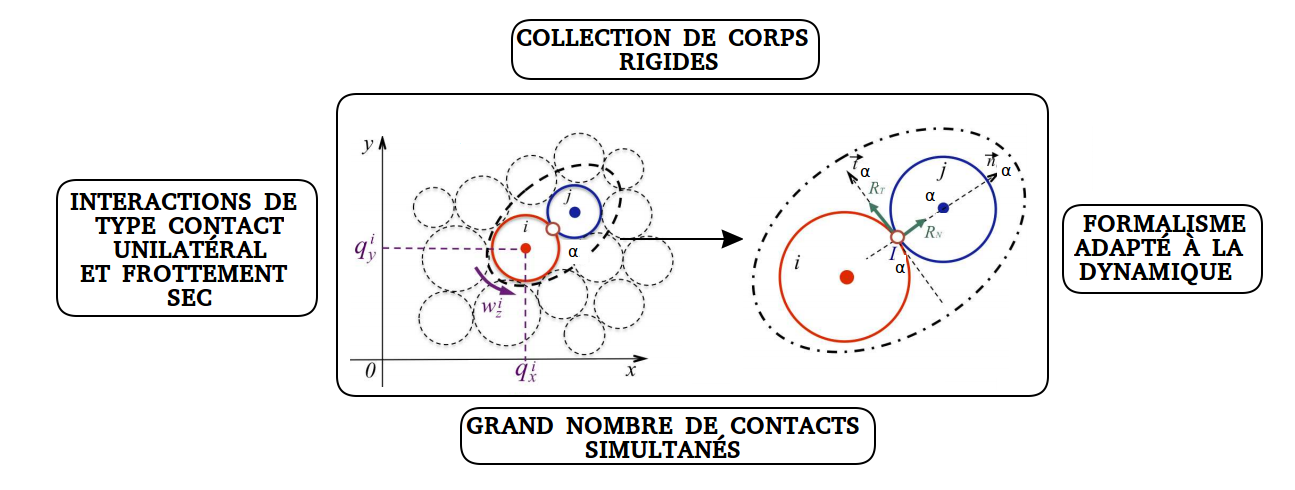
\includegraphics[width=0.9\textwidth]{chapitres/chapitre_3/figures/global_local_schema.png}
    \caption{\centering Schématisation du passage de l'espace global des particules à l'espace local des contact.}\label{fig31}
\end{figure}

Dans un modèle à corps rigides, la dynamique des contacts, qui donnera lieu à la méthode \textit{Contact Dynamics} (CD), aussi connue sous le nom de \textit{Non-Smooth Contact Dynamics} (NSCD), est basée sur la DEM, initialement développée pour la simulation de matériaux granulaires, et issue d'une formulation mathématique de la dynamique non-régulière et des développements algorithmiques réalisés par J. J. Moreau et M. Jean \cite{jean1992unilaterality, moreau1977application, moreau1988unilateral, moreau1994numerical, moreau1999sweeping}. À la différence de la méthode \textit{Molecular Dynamics} (MD) où les les contacts entre corps rigides sont conformes et obéissent à un comportement visco-élastique, les contacts induisent des forces non-régulières dans la méthode NSCD. Nous pouvons nous référer à \cite{radjai2009contact} pour plus de détails. 

\subsection{Lois de contacts non-régulières}

\subsubsection{Conditions de contacts}

Dans ce qui suit, nous allons considérer une collection dynamique de corps rigides impliqués dans plusieurs contacts simultanés. Le cadre décrit précédemment, constitué des deux repères global et local, nous sert de point de départ pour la modélisation de ces milieux. Nous nous focaliserons exclusivement sur les interactions de type contact unilatéral et frottement sec. Sous ces hypothèses, les conditions de contact sont formulées en termes de vitesse pour ne pas avoir de dissipation dû au schéma, reliant ainsi les impulsions aux vitesses. Il s'agit alors de prédire les vitesses des corps et les impulsions agissant sur les différents points de contact.\\

Partant de là, l'interaction mécanique résultant d'une collision potentielle entre une particule rigide $i$ et sa voisine $j$, consiste en un contact ponctuel $\alpha$ ($\alpha$ étant un contact de l'ensemble des noeuds de contact $\cal S$). La description mécanique du contact potentiel $\alpha$ mettant en jeu les deux particules rigides $P_i$ (de masse $m_i$, de centre de masse $G_i$) et $P_j$ (de masse $m_j$, de centre de masse $G_j$), nommés par convention candidat et antagoniste, laisse supposer l'existence d'un plan de contact unique en 3D (droite en 2D) tangent aux deux particules au point de contact $\alpha$, et peut être géométriquement défini de sorte que le contact puisse être doté d'un repère local défini par un vecteur unitaire normal $\vect{n}$ et deux vecteurs unitaires tangentiels orthogonaux $\vect{t_1}$ et $\vect{t_2}$ (un vecteur unitaire tangentiel $\vect{t}$ en 2D). L'orientation des axes est une question de commodité (voir Figure \ref{fig32}). Nous utilisons la notation $\vect{u}$ et $\vect{p}$ pour le déplacement local et le tenseur d'impulsion local au point de contact $\alpha$ respectivement (un point en exposant représente la dérivée par rapport au temps $t$, e.g.\ $\dot{u} ={\partial u}/{\partial t}$). On note également $\dot{u}_n$ et $\vect{\dot{u}}_t$ les composantes normale et tangentielle de la vitesse $\vect{\dot{u}}$ définie par $\dot{u}_n=\vect{\dot{u}}\cdot\vect{n}$, $\vect{\dot{u}}_t=\vect{\dot{u}}-u_n\vect{n}$. Enfin, $p_n$ et $\vect{p}_t$ représentent les impulsions de contact normale et tangentielle sur le point de contact, définies par $p_n=(\vect{p}\vect{n})\cdot\vect{n}$ et $\vect{p}_t =
\vect{p}\vect{n} - p_n \vect{n}$.
 
\begin{figure}[!h]
  \centering
    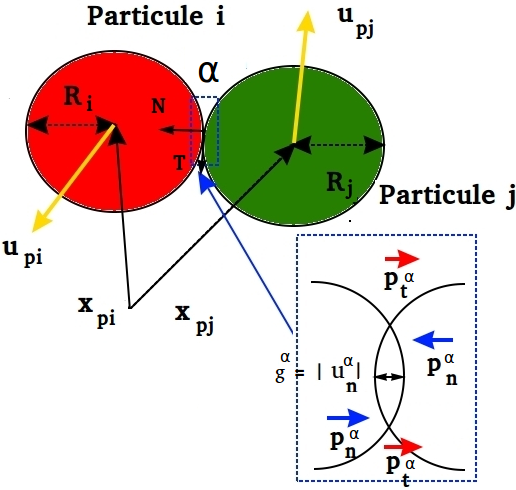
\includegraphics[width=0.8\textwidth]{chapitres/chapitre_3/figures/contact_Pi_Pj.png}
    \caption{Modélisation d'un problème de contact multi-corps rigides.}\label{fig32}
\end{figure}

Lorsque la distance $u_n$ entre une particule $P_i$ et sa projection sur une autre particule $P_j$ (appelée gap $g^{\alpha}$) reste positive (contact potentiel non abouti), aucune contrainte n'est exercée et par conséquent, l'impulsion de contact normale $p_n$ est nulle. Mais dès que le gap $u_n$ devient nul (contact potentiel abouti), une impulsion de contact normale $p_n$ répulsive se crée au point de contact $\alpha$, sa valeur dépend des forces qui agissent sur les deux particules (voir Figure \ref{fig32}). Ces conditions définissent une première relation complémentarité, appelée loi de Signorini en vitesse \cite{signorini1933sopra}, reliant la vitesse normale $\dot{u}_n$ à l'impulsion de contact normale $p_n$. Ces conditions de contact peuvent être écrites comme suit:


\begin{eqnarray}
&&\label{undc0} \mbox{Si} \quad g^{\alpha} > 0 \quad \mbox{alors} \quad p^{\alpha}_n = 0,\\[2mm]
&&\nonumber \mbox{Si} \quad g^{\alpha} \leq 0 \quad \mbox{alors} \\[2mm]
&&\label{undc1} \qquad \qquad \qquad \qquad\dot{u}^{\alpha}_n \ge 0,\\[2mm]
&&\label{undc2} \qquad \qquad \qquad  \qquad p^{\alpha}_n \ge 0,\\[2mm]
&&\label{perstce} \qquad \qquad \qquad  \qquad\dot{u}^{\alpha}_n p^{\alpha}_n = 0,
\end{eqnarray}

Les relations (\ref{undc0}) -- (\ref{perstce}) conduisent aux conditions d'une loi de contact complète formulée par Moreau. La dernière condition (\ref{perstce}), est une relation de complémentarité qui assure la conservation de l'énergie (voir \cite{dubois2018contact} pour plus de détails). Cette condition, également appelée condition de persistance, signifie qu'une impulsion de contact normale $p_n$ n'apparaît que lors d'un contact persistant, et doit être ajoutée afin de faire disparaître le travail des impulsions de contact normales au temps $t$ et préserver la quantité d'énergie avant et après le choc. J.-J. Moreau a prouvé que ces conditions assurent la non-interpénétrabilité entre les corps; voir le Lemme de viabilité de Moreau (cf \cite{moreau1994numerical, moreau1999sweeping}).

\begin{figure}[!h]
  \centering
    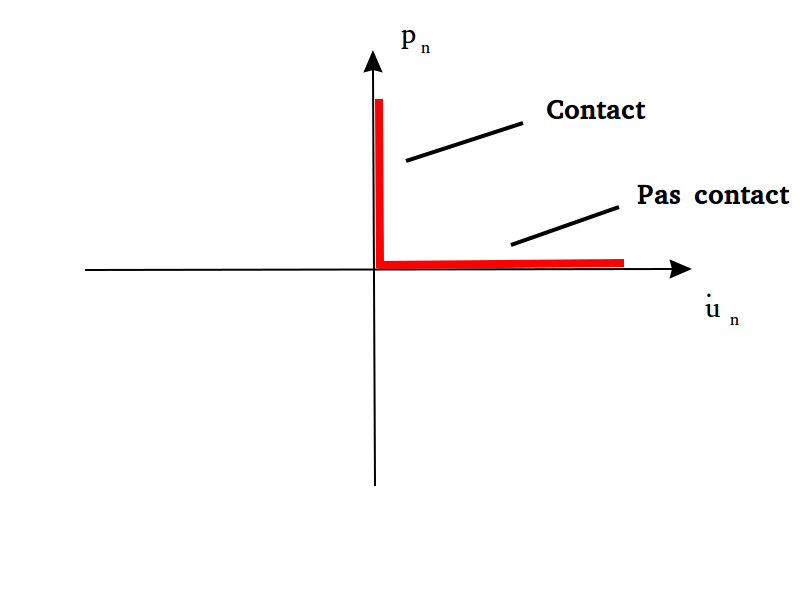
\includegraphics[width=0.6\textwidth]{chapitres/chapitre_3/figures/signorini_complementarity_relation.png}
    \caption{Relation de complémentarité de Signorini.}\label{fig3}
\end{figure}

D'autre part, du fait de la non-régularité du mouvement, la vitesse $\dot{u}_n(t)$ n'est pas unique. En effet, nous distinguons la vitesse par limite inférieure $\dot{u}_n^{-}$ et la vitesse par limite supérieure $\dot{u}_n^{+}$ qui, dans un schéma d'intégration pas à pas (\textit{time stepping scheme}), doivent être considérées comme les vitesses de contact aux instants $t$ et $t + \delta{t}$, respectivement. La vitesse réelle est alors sans importance puisque seules les vitesses $\dot{u}_n^{-}$ et $\dot{u}_n^{+}$ (et les sauts de vitesse) sont prises en compte dans la dynamique. Par analogie avec une collision binaire impliquant 2 particules rigides, la principale inconnue du problème est $\dot{u}_n^{+}$ connaissant la vitesse d'approche juste avant le contact $\dot{u}_n^{-}$ attribuée au début du pas de temps dans un schéma d'intégration pas à pas. Le contact dépend donc du choix de la vitesse $\dot{u}_n$ et de la nature de la contrainte $p_n$ impliquée dans les relations de complémentarité (\ref{undc0}) -- (\ref{perstce}) de la loi de contact unilatérale en vitesse sans frottement.

Le calcul de cette vitesse $\dot{u}_n$ est physiquement motivé par un choix simple qui consiste à supposer que c'est une moyenne pondérée entre $\dot{u}_n^{-}$ et $\dot{u}_n^{+}$:\\
$\dot{u}_n = \eta \dot{u}_n^{-} + (1 - \eta) \dot{u}_n^{+}$, où $\eta$ est un paramètre du matériau caractérisant le contact. Pour plus de détails sur ce choix, voir \cite{radjai2009contact}. Ainsi, Pour $\eta \ne 0$, un choc binaire entre deux particules rigides implique $\frac{-\dot{u}_n^{+}}{\dot{u}_n^{-}} = \frac{\eta}{(1-\eta)}$. En identifiant ce rapport avec le coefficient de restitution normal du matériau $e_n$, nous obtenons $\eta = \frac{e_n}{(1+e_n)}$. Par conséquent, nous définissons:

\begin{equation}
\dot{u}_n = \frac{\dot{u}_n^{+} + e_n \dot{u}_n^{-}}{(1+e_n)}
\label{velocity_after}
\end{equation}

Par ailleurs, une condition géométrique de non-interpénétrabilité s'ajoute à la loi de contact unilatérale sans frottement du fait de la rigidité des particules, et implique une non-régularité temporelle à cause des sauts de vitesse (discontinuité).

\subsubsection{Loi de frottement de Coulomb}

Outre les relations de complémentarité et conditions de persistance et de non-interpénétrabilité dues à la non-régularité du mouvement de choc entre deux particules rigides, la loi de frottement de Coulomb \cite{desplanques2015amontons} s'ajoute à la liste de comportements aux contacts complexes. Par définition, cette relation relie la composante tangentielle de contact (ou force de frottement) $\vect{p}_t$ à la composante tangentielle de vitesse $\vect{\dot{u}_t}$ au point de contact $\alpha$. La loi de frottement de Coulomb peut être énoncée en utilisant la forme algorithmique suivante (voir la Figure 4 pour une représentation graphique):

\begin{eqnarray}
&&\label{fricon} \vect{p}^{\alpha}_t \neq \bzero.\\[2mm]
&&\label{fricdc_gran} \left\{\begin{array}{ll}
p^{\alpha}_n = 0 \Longrightarrow \dot{u}^{\alpha}_n \ge 0, \quad (Non\ contact)\\[2mm]
p^{\alpha}_n > 0 \quad et \quad ||\vect{p}^{\alpha}_t|| < \mu p^{\alpha}_n \Longrightarrow \vect{\dot{u}^{\alpha}_t} = 0,  \quad (Adhérence)\\[2mm]
p^{\alpha}_n > 0 \quad et \quad ||\vect{p}^{\alpha}_t|| = \mu p^{\alpha}_n \Longrightarrow \exists \beta \ge 0, \vect{\dot{u}^{\alpha}_t} = \beta \frac{\vect{p}^{\alpha}_t}{||\vect{p}^{\alpha}_t||}  \quad (Glissement).
\end{array}\right.
\end{eqnarray}

\begin{figure}[!h]
  \centering
    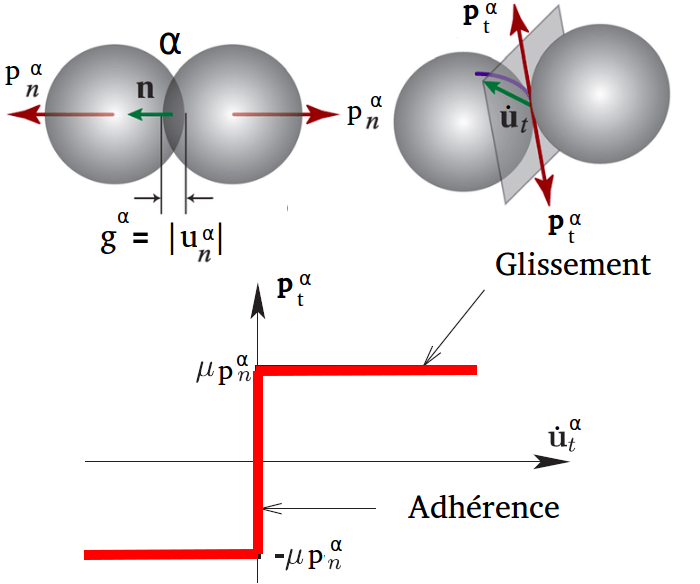
\includegraphics[width=0.55\textwidth]{chapitres/chapitre_3/figures/loi_frottement_coulomb.png}
    \caption{\centering Conditions de Coulomb.}\label{fig4}
\end{figure}

\noindent où $\mu$ le coefficient de frottement dynamique. On notera que lorsqu'il y a adhérence, le frottement est dit statique, tandis que lorsqu'il y a glissement, le frottement est dynamique.

Comme cela a été vu pour la loi de Signorini dans le paragraphe précédent, le calcul de la vitesse tangentielle $\vect{\dot{u}_t}$ à partir des conditions de frottement suit le même principe. La force de frottement tangentielle $\vect{p}_t$ représente l'effet moyen des forces statiques et répulsives relatives au contact pendant un laps de temps $\delta_t$. La vitesse tangentielle $\vect{\dot{u}_t}$ est alors une vitesse moyenne (voir \cite{radjai2009contact}). Dans le même esprit que pour les réactions de contact normales, un modèle simple cohérent avec la coefficient de restitution tangentiel consiste à définir $\vect{\dot{u}_t}$ de la façon suivante:

\begin{equation}
\vect{\dot{u}_t} = \frac{\vect{\dot{u}_t}^{+} + e_t \vect{\dot{u}_t}^{-}}{(1+e_t)}
\label{8}
\end{equation}

Dans ce qui suit, deux couples $(\dot{u}_{n}^{\alpha},p_{n}^{\alpha})$ et $(\vect{\tilde{\dot{u}}}^{\alpha},\vect{p}^{\alpha})$ vérifiant ces ensembles de conditions pour un noeud de contact potentiel $\alpha$ sont notés comme suit:

\begin{eqnarray}
&& \left\{\begin{array}{lll}
contact\_law(\dot{u}_{n}^{\alpha},p_{n}^{\alpha}) = .true.\\[2mm]
friction\_law(\vect{\tilde{\dot{u}}}^{\alpha},\vect{p}^{\alpha}) = .true.\\[2mm]
\end{array}\right.
\label{unifriclaw}
\end{eqnarray}

\noindent où $contact\_law(\dot{u}_{n}^{\alpha},p_{n}^{\alpha})$ décrit les conditions de contact unilatérales ((\ref{undc0}) -- (\ref{perstce})), tandis que $friction\_law(\vect{\tilde{\dot{u}}}^{\alpha},\vect{p}^{\alpha})$ décrit la loi de frottement de Coulomb ((\ref{fricon}) -- (\ref{fricdc_gran})).

\subsection{Gestion des interactions non-régulières NSCD}

Comme nous l'avons vu précédemment, le contact entre corps rigides entraîne une non-régularité en loi entre la force de contact et la vitesse relative locale du choc à cause du frottement, et une non régularité temporelle à cause des sauts de vitesse avant et après le choc. La formulation NSCD permet alors de simuler le comportement complexe de ces corps rigides. Il est alors possible de résoudre, sur un pas de temps, de
nombreux contacts simultanés. Pour cela, deux tâches principales de calcul sont prévues:

\begin{itemize}
    \item \textbf{Au niveau global}, une intégration temporelle implicite des équations de mouvement;
    \item \textbf{Au niveau local}, un traitement explicite qui gère l’évolution du réseau de contact entre les corps rigides.
\end{itemize}

Dans cette partie, qui reprend et complète les travaux de Barboteu et Dumont \cite{barboteu2018primal}, nous présentons d'abord les équations de mouvement régissant la dynamique multi-contacts des corps rigides, ensuite, nous décrivons les différentes tâches de calcul relatives à la formulation NSCD afin de proposer un algorithme général dans lequel les conditions de contact unilatéral et de frottement de Coulomb vues dans (\ref{undc0}) -- (\ref{fricdc_gran}) sont traitées numériquement.

\subsubsection{Équations de mouvement}

Pour décrire le mouvement d'un système multi-contact entre corps rigides, on introduit des notations spécifiques. Partant du principe qu'une particule $P$ parmi $N_p$ particules est décrite par la position de son centre de gravité et par sa rotation, nous noterons $\vect{q}$ la coordonnée généralisée décrivant sa position dans l'espace, ($q \in \mathbb{R}^{\Bar{d} \times N_p}$, où $\Bar{d} = 6$ pour un problème 3D et $\Bar{d} = 3$ pour un problème 2D), $\vect{\dot{q}}$ sa vitesse généralisée et $d\vect{\dot{q}}$ sa différentielle associée. D'après le principe fondamental de la dynamique, les équations de mouvement formulées en terme de mesures différentielles peuvent s'écrire comme suit:

\begin{equation}
\mathbb{M} d\vect{\dot{q}} + \bF^{int}(t,\vect{q},\vect{\dot{q}})dt = \bF^{ext}(t,\vect{q},\vect{\dot{q}})dt + d\bR
\label{eqmotion}
\end{equation}

\noindent où
\begin{itemize}
    \item $\mathbb{M}$ représente la matrice des masses généralisée,
    \item $\bF^{int}$ et $\bF^{ext}$ représentent les forces intérieures et extérieures s'exerçant sur le système,
    \item $d\bR$ une mesure réelle non négative représentant les impulsions de contact entre particules 
\end{itemize}

Pour des raisons de simplicité, seules les forces extérieures seront considérées pour la suite.

\subsubsection{Schéma de discrétisation temporelle}

Dans une approche de discrétisation temporelle (\textit{time stepping scheme}), nous considérons un intervalle de temps pris entre $[0,T]$ que nous discrétisons en introduisant:
$t_{k+1} = t_k + \Delta{t}\ pour\ k = 0,...,N_T - 1$ où,

\begin{itemize}
    \item $\Delta{t} = T / N_T$: le pas de temps
    \item $N_T$: le nombre de pas de temps
\end{itemize}

Ensuite, l'équation (\ref{eqmotion}) est intégrée sur chaque intervalle de temps $[t_k,t_{k+1}]$, et approchée en utilisant un $\theta$-schéma avec $\theta \in [\frac{1}{2},1]$ pour des raisons de stabilité (voir \cite{moreau1999sweeping, renouf2005conjugate}). Par conséquent, la discrétisation temporelle de l'équation (\ref{eqmotion}) donne:


\begin{eqnarray}
&& \left\{\begin{array}{lll}
\mathbb{M} (\vect{\dot{q}}_{k+1} - \vect{\dot{q}}_{k}) =  
\Delta{t}(\theta \bF_{k+1} + (1 - \theta)\bF_k) + \bP_{k+1},\\[2mm]
\vect{q}_{k+1} = \vect{q}_{k} + \Delta{t} \theta \vect{\dot{q}}_{k+1} + \Delta{t} (1 - \theta) \vect{\dot{q}}_{k}.\\[2mm]
\end{array}\right.
\label{eqmotiondiscr}
\end{eqnarray}

où $\bP_{k+1}$ représente la valeur de l'impulsion totale sur le pas de temps, et $\bF_k$ (respectivement $\bF_{k+1}$) est la force extérieure calculée au temps $t_k$ (respectivement $t_{k+1}$).\\
Nous noterons $\vect{\dot{q}}_{k}^{free} = \vect{\dot{q}}_{k} + \mathbb{M}^{-1} \Delta{t}(\theta \bF_{k+1} + (1 - \theta) \bF_{k})$ la vitesse libre (vitesse sans impulsions de contact). Par suite, la première équation de (\ref{eqmotiondiscr}) s'écrit:

\begin{equation}
\vect{\dot{q}}_{k+1} = \vect{\dot{q}}_{k}^{free} + \mathbb{M}^{-1} \bP_{k+1}
\label{freevel}
\end{equation}

\subsubsection{Passage de l'espace des particules à l'espace des contacts}

En dynamique des contacts non réguliers NSCD, les impulsions de contact ne sont pas des fonctions explicites qui définissent l'état d'équilibre du système étudié. Par conséquent, les impulsions et les vitesses doivent être déterminées en même temps. Comme les lois de contact et de frottement \ref{unifriclaw} sont exprimées à l'aide des variables de contact, nous devons exprimer les équations de mouvement à l'aide de ces mêmes variables.\\
Un simple passage du repère global au repère local à chaque contact, désigné par $\alpha \in [1,N_{\alpha}]$ (où $N_{\alpha}$ est le nombre total de contacts) relatif à un noeud de contact $x_{\alpha}$ ($1 \leq \alpha \leq N_{\alpha}$) nous permet d'écrire la loi de contact qui lui est relative. Comme les vitesses des particules, les vitesses de contact $u^{\alpha}_n$ et $u^{\alpha}_t$ peuvent être collectées dans un vecteur colonne $u \in \mathbb{R}^{d \times N_c}$ (où $d = 3$ pour un problème 3D et $d = 2$ pour un problème 2D). De la même manière, les impulsions de contact $p^{\alpha}_n$ et $\vect{p}^{\alpha}_t$ sont représentées par un vecteur $\vect{p} \in \mathbb{R}^{d \times N_c}$. Nous aimerions donc transformer les équations de la dynamique vues en (\ref{eqmotiondiscr}) de $\vect{P}$ et $\vect{\dot{q}}$ en $\vect{p}$ et $\vect{\dot{u}}$.\\
%Pour alléger les notations et dans un soucis de simplification, les équations de la dynamique (\ref{eqmotiondiscr}) sont converties en une seule équation matricielle dont voici l'expression:

%\begin{equation}
%\mathbb{M} (\vect{\dot{q}}^{+} - \vect{\dot{q}}^{-}) =  
%\Delta{t}(\bF + \bF_{ext})
%\label{13}
%\end{equation}
Puisque les vitesses de contact $\vect{\dot{u}}$ sont linéaires en vitesses de particules $\vect{\dot{q}}$, la transformation des vitesses est une application affine:

\begin{equation}
\vect{\dot{u}}^{\alpha} = H^{*}(\vect{q},\alpha) \vect{\dot{q}}
\label{14}
\end{equation}

où $\vect{\dot{u}}^{\alpha}$ est la vitesse relative locale entre les deux particules en contact $P_i$ et $P_j$, $H^{*}(\vect{q},\alpha)$ la matrice $d N_c \times \Bar{d} N_p$ contenant essentiellement des informations sur la géométrie du réseau de contacts. Une application linéaire similaire relie $\vect{p}$ à $\vect{P}$:

\begin{equation}
\vect{P} = H(\vect{q},\alpha) \vect{p}^{\alpha}
\label{15}
\end{equation}

où $\vect{p}^{\alpha}$ représente les impulsions au contact $\alpha$, $H(\vect{q},\alpha)$ la matrice $\Bar{d} N_p \times d N_c$ de passage entre les deux repères qui permet de déterminer les variables $\vect{\dot{u}}^{\alpha}$ et $\vect{p}^{\alpha}$ dans le repère local relatif au noeud de contact $x_{\alpha}$ à partir des variables globales $\vect{\dot{q}}$ et $\vect{P}^{\alpha}$.\\ 
La matrice $H$, que nous appellerons plus communément matrice locale-globale de contact, contient les mêmes informations que $H^*$ dans un contexte de dualité ou de symétrie:
 
 \begin{equation}
H = H^{*T}
\label{16}
\end{equation}

\noindent où $H^{*T}$ est la transposée de $H^*$.\\
On rappelle que $\vect{p}^{\alpha}$ peut être décomposé en la somme d'une composante normale $p^{\alpha}_n$ et d'une composante tangentielle $\vect{p}^{\alpha}_t$ comme suit:
$\vect{p}^{\alpha} = p^{\alpha}_n \vect{n} + \vect{p}^{\alpha}_t$. Puisque le changement de repère local-global est calculé pour chaque noeud de contact $\alpha$, le passage local-global total permet de calculer toutes les vitesses et impulsions de contact. On note alors $\mathbb{H}(q)$ la matrice de passage locale-globale totale ou généralisée, pour $\vect{\dot{u}}^{\alpha}$ et $\vect{p}^{\alpha}$ dans $\mathbb{R}^{d \times N_c}$ (vecteurs composés respectivement de toutes les vitesses relatives et impulsions de contact):

\begin{eqnarray}
&& \left\{\begin{array}{lll}
\vect{\dot{u}} = \mathbb{H}^{*}(\vect{q}) \vect{\dot{q}},\\[2mm]
\vect{P} = \mathbb{H}(\vect{q}) \vect{p}.\\[2mm]
\end{array}\right.
\label{17}
\end{eqnarray}

Le schéma récapitulatif de cette transformation des équations de la dynamique des particules aux équations de transfert est présenté dans la Figure \ref{passage_loc_glob}.

\begin{figure}[!h]
  \centering
    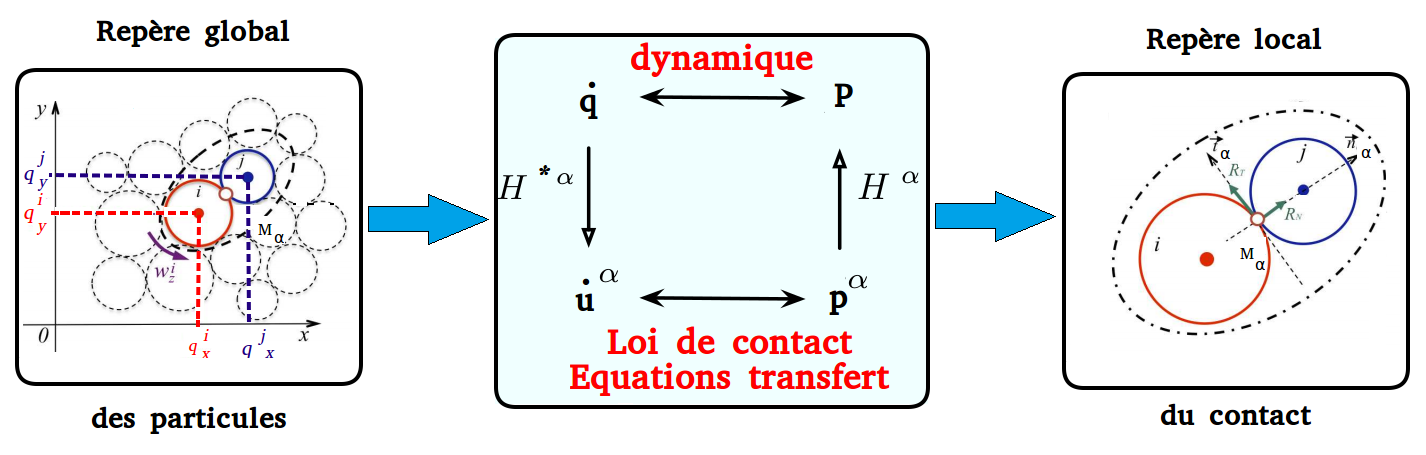
\includegraphics[width=0.9\textwidth]{chapitres/chapitre_3/figures/matrice_passage_glob-loc.png}
    \caption{Schéma du passage de la dynamique globale des particules à la dynamique locale relative aux contacts.}\label{passage_loc_glob}
\end{figure}

En combinant les équations (\ref{freevel}) et (\ref{17}), la discrétisation du mouvement d'un système multi-contacts entre corps rigides peut s'écrire comme suit:

\begin{eqnarray}
&& \left\{\begin{array}{lll}
\vect{\tilde{\dot{u}}}_{k+1} = \vect{\tilde{\dot{u}}}_{k}^{free} + \mathbb{W} \vect{p}_{k+1},\\[2mm]
contact\_law(\tilde{\dot{u}}_{n,k+1}^{\alpha},p_{n,k+1}^{\alpha}) = .true. \quad \forall \alpha \in [1,...,N_{\alpha}],\\[2mm]
friction\_law(\vect{\tilde{\dot{u}}}_{k+1}^{\alpha},\vect{p}_{k+1}^{\alpha}) = .true. \quad \forall \alpha \in [1,...,N_{\alpha}].\\[2mm]
\end{array}\right.
\label{contact_friction_laws}
\end{eqnarray}

où $\mathbb{W} = \mathbb{H}^{*} \mathbb{M}^{-1} \mathbb{H}$ est l'opérateur de Delassus, et $\vect{\tilde{\dot{u}}}_{k}^{free} = \mathbb{H}^{*} \vect{\dot{q}}_{k}^{free}$ est la vitesse libre relative sans contact. On notera que la loi de choc de Newton est également considérée dans la première équation de (\ref{contact_friction_laws}) (voir \cite{moreau1988unilateral}), qui modifie $\vect{\dot{u}}_{k}$ et $\vect{\dot{u}}_{k}^{free}$ en $\vect{\tilde{\dot{u}}}_{k}$ et $\vect{\tilde{\dot{u}}}_{k}^{free}$ respectivement. Les deux dernières équations de (\ref{contact_friction_laws}) représentent les lois de contact et de frottement implicite exprimées à l'aide des variables locales  relatives au contact $\alpha$ et qui sont dans notre cas les conditions classiques des lois de Signorini et de Coulomb avec $\vect{p}^{\alpha}_t \neq 0$.

\subsection{Algorithme général de résolution NSCD: Méthode de Gauss-Seidel non-linéaire (NLGS)}\label{NLGS}

\subsubsection{Description de l'algorithme}\label{NSCD_algo}

Ce paragraphe est consacré à la description détaillée de l'algorithme utilisé au niveau global pour résoudre les problèmes de contact dynamique multi-corps rigides. Selon Jean et Moreau (voir \cite{jean1999non, jourdan1998gauss, moreau1988unilateral}), nous utilisons l'algorithme NLGS qui consiste à considérer successivement chaque contact jusqu'à la convergence. Le schéma temporel pas à pas combiné à l'algorithme NLGS prend la forme suivante:

\begin{itemize}
\item Boucle sur le pas de temps $k$
\begin{itemize}
\item Prédiction d'une position intermédiaire (pour le changement de repère local-global): \\
\begin{equation}\label{globalmapapp1}
{\bf q}_{k+\frac12}={\bf q}_k+\frac{\Delta t}{2}\qp_k;
\end{equation}
\item Initialisation du mouvement: $\qp^{0}_{k+1}=\qp_{k}^{free}$%+{\mathbb M}^{-1}{\bf F}\Delta t$ 
(initialisation des impulsions de contact avec ${\bf P}=0$).
\item  Boucle sur $j\geq 0$ (NLGS), jusqu'à convergence
\begin{itemize}
\item Boucle sur les contacts $\alpha$:
\begin{itemize}
\item Calcul du changement de repère local-global
\begin{equation}\label{globalmapapp2}
\dot{\bf  u}^-=H^*({\bf q}_{k+\frac12},\alpha)\dot{\bf{q}}_k\ ;
\end{equation}
\begin{equation}
\dot{\bf u }^{\alpha,j,+}=H^{*}({\bf q}_{k+\frac12},\alpha)\dot{\bf{q}}^{j}_{k+1}
\end{equation}
\item Loi de choc de Newton (Formalisme de Moreau exprimé en vitesse)
\begin{equation}\label{newtonlawen}
\tilde{\dot{u}}_n^{\alpha,j+1}=\frac{\dot{u}_n^{\alpha,j,+}+e_n \dot{u}_n^-}{1+e_n};
\end{equation}
\begin{equation}\label{newtonlawet}
\vect{\tilde{{\dot{u}}}}_t^{\alpha,j+1}=\frac{\vect{\dot{\bf u}}_t^{\alpha,j,+}+e_t{\vect{\dot{\bf u}}}_t^{-}}{1+e_t}
\end{equation}
\item Calcul de la loi de contact et frottement:
\begin{eqnarray}
&& \left\{\begin{array}{lll}
contact\_law(\tilde{\dot{u}}_{n}^{\alpha,j+1},p_{n}^{\alpha,j+1}) = .true. \\[2mm]
friction\_law(\vect{\tilde{\dot{u}}}^{\alpha,j+1},\vect{p}^{\alpha,j+1}) = .true. \\[2mm]
\end{array}\right.
\label{18}
\end{eqnarray}
\item Actualisation des vitesses globales:
\begin{equation}\label{new_vel}
\qp^{j+1}_{k+1}=\qp_{k+1}^{j}+{\mathbb M}^{-1}P({\bf q}_{k+\frac12},\alpha) \vect{p}^{\alpha,j+1}
\end{equation}
\end{itemize}
\item Fin de la boucle sur les contacts $\alpha$.
\end{itemize}
\item Fin de la boucle sur $j$ (NLGS). Lorsque la convergence est atteinte, actualisation des vitesses: $\qp_{k+1}=\qp_{k+1}^{j+1}$
\item Actualisation des déplacements généralisés: ${\bf q}_{k+1}={\bf q}_{k+\frac12}+\frac{\Delta t}{2}\qp_{k+1}$
\end{itemize}
\item Fin de la boucle en temps $k$.
\end{itemize}

\subsection{Résolution numérique des problèmes multi-contacts}

Nous avons vu dans le paragraphe précédent que la formulation d'un problème en dynamique des contacts non-réguliers est décrite en terme:

\begin{itemize}
    \item d'équations discrétisées de la dynamique pour chaque corps rigides au niveau global (\ref{freevel}),
    \item de lois de contact exprimées au niveau local pour chaque contact $\alpha$ (\ref{contact_friction_laws}),
    \item de changement de repère local-global à l'aide des matrices de contact $\mathbb{H}$ et $\mathbb{H}^{*}$.
\end{itemize}

Par une suite de transformations algébriques, on condense de manière explicite les équations discrétisées de la dynamique (\ref{freevel}) pour ainsi obtenir un système local à résoudre pour chaque contact $\alpha$ (voir système \ref{contact_friction_laws}).\\
Une fois le problème formulé, il s'agit de le résoudre numériquement par une méthode adéquate.

\subsubsection{Problème global}

Comme cela a été évoqué précédemment, la formulation NSCD repose sur une première tâche de calcul au niveau global qui consiste à intégrer de manière implicite sur chaque pas de temps les équations de mouvement, et ce, afin de résoudre les contacts de manière simultanée. Suivant les idées de Jean et Moreau (voir \cite{jean1999non, jourdan1998gauss, moreau1988unilateral}), l'approche NSCD classique repose sur un algorithme de Gauss-Seidel non-linéaire (NLGS). La méthode de résolution est comparable à un algorithme de Gauss-Seidel:

\begin{itemize}
    \item pour chaque contact $\alpha$ on résout en fixant les contributions des autres contacts ($\beta \neq \alpha$),
    \item la résolution du problème (lois de contact et de frottement) fait l'objet d'un traitement local explicite non-linéaire qui gère l'évolution du réseau de contacts entre les corps rigides,
    \item On effectue le nombre d’itérations NLGS, où on passe en revue tous les contacts jusqu'à la convergence.
\end{itemize}

\subsubsection{Problème local}

Le problème local, consacré à la résolution de la loi de contact et frottement en tenant compte de la loi de Newton au niveau local, consiste à déterminer numériquement les impulsions de contacts locales (voir système (\ref{contact_friction_laws}). Dans le cas des systèmes multi-corps rigides, les conditions de contact formulées en vitesse (\ref{undc0}) -- (\ref{perstce}) sont toujours utilisées et relient les impulsions de contacts aux vitesses. Dans cette perspective, il s'agit de prédire les vitesses des corps et les impulsions de contact agissant sur les contacts simultanés. En d'autres termes, il s'agit de trouver les couples $(\tilde{\dot{u}}_{n}^{\alpha},p_{n}^{\alpha})$ et 
$(\vect{\tilde{\dot{u}}}_{t}^{\alpha},\vect{p}_{t}^{\alpha})$ pour lesquels la loi de contact et frottement sont vraies.\\
Dans la littérature, deux méthodes numériques classiques ont été développées afin de résoudre les problèmes de contacts NSCD avec frottement, la méthode du Lagrangien augmenté standard (voir \cite{alart1991mixed}), combinée à une méthode de Newton généralisée pour résoudre des équations non différentiables résultant de problèmes de contact avec frottements, et la méthode du bi-potentiel amélioré, introduite par Saxcé et Feng dans \cite{de1991new} et \cite{fortin2002improved}. En ce qui nous concerne, l'approche Active Set  pour la résolution de problèmes multi-contacts, initiée en milieu déformable, et introduite dans le chapitre précédent fera l'objet d'une étude détaillée en milieu multi-corps rigides dans la suite de ce manuscrit.

\subsubsection{Stratégie de résolution}

La formulation NSCD décrite par l'algorithme vu en \ref{NSCD_algo}, couplée au solveur itératif NLGS, permet d'examiner successivement tous les contacts jusqu'à convergence, chaque contact étant traité séparément en utilisant le formalisme numérique PDAS pour calculer les impulsions de contact locales sur chaque ensemble de contacts dit "Actif". La Figure \ref{schema_nscd} est une schématisation de la stratégie de résolution d'un problème de contact dynamique multi-corps rigides:

\begin{figure}[!h]
  \centering
    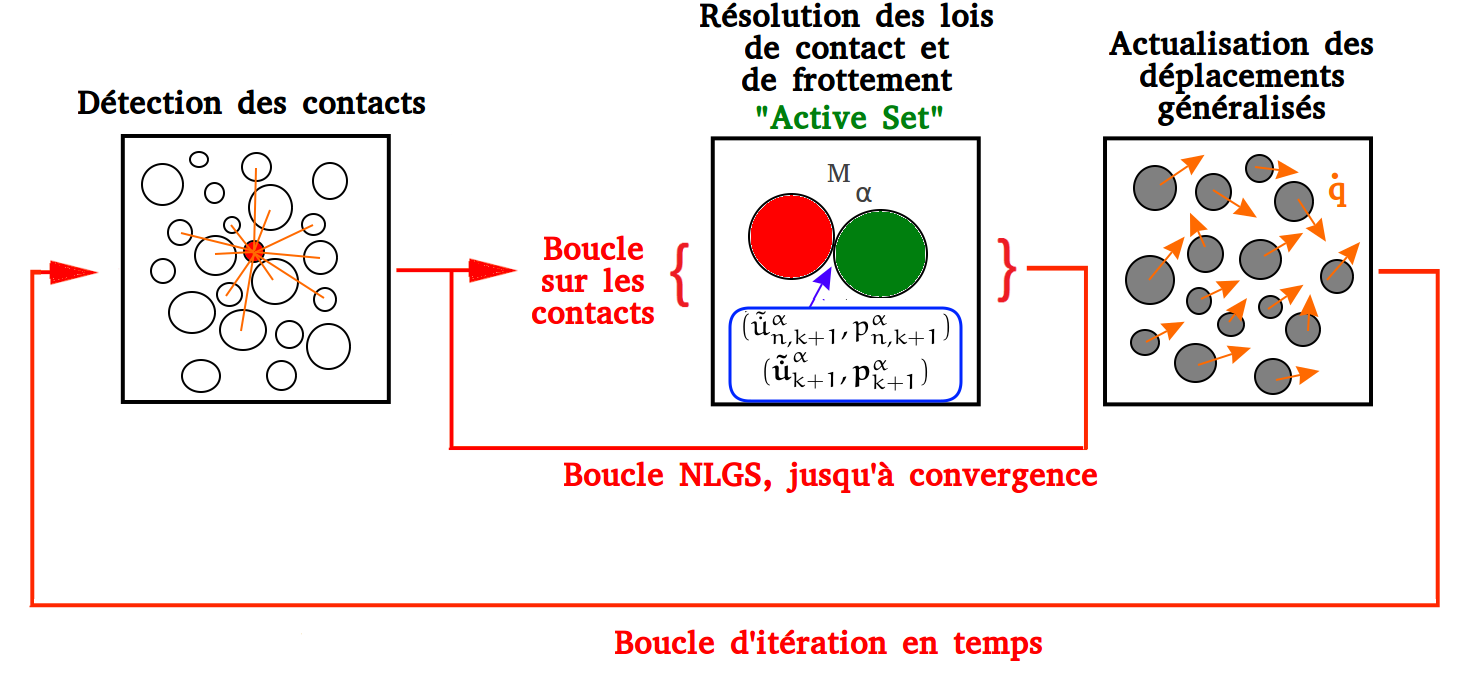
\includegraphics[width=0.9\textwidth]{chapitres/chapitre_3/figures/nscd_resolution.png}
    \caption{\centering Stratégie de résolution d'un problème de contact dynamique multi-corps rigides.}\label{schema_nscd}
\end{figure}

\section{Méthode Primal-Dual Active Set pour la NSCD}\label{PDAS_4_NSCD}

\subsection{Active Set et dynamique non-régulière}

Dans le cadre de la résolution des contacts dynamiques non-réguliers NSCD entre corps rigides, nous avons vu précédemment tout l'intérêt de la formulation NSCD pour la simulation du comportement dynamique d'une collection de corps rigides telle que les milieux granulaires. Basée essentiellement sur deux tâches principales de calcul, le niveau global permet de résoudre les équations de mouvement, tandis que le niveau local est consacré à la résolution de contact. Et c'est à ce niveau de calcul qu'interviennent les méthodes PDAS qui, par un traitement numérique de chaque condition de contact, permettent de résoudre les lois de contact et de frottement décrivant la dynamique de ces milieux discrets. Ce paragraphe est donc consacré au traitement numérique des conditions de contact par une méthode PDAS dans le cadre d'un problème de contact dynamique multi-corps rigides.

\subsection{Approche de Newton semi-régulière}\label{semi-smooth_newton}

\subsubsection{Fonction de complémentarité de contact}\label{func_comp_cont}

\noindent Les conditions de contacts de Signorini en vitesse (\ref{undc1})--(\ref{perstce}) sont représentées par la fonction de complémentarité non-linéaire suivante 
\begin{align}\label{fcomp1}
{\cal C}_{n}^{\vect{p}}(\dot{u}^{\alpha}_n,p^{\alpha}_n)=p^{\alpha}_n - [p^{\alpha}_n - \gamma_n \dot{u}^{\alpha}_n]_+ \quad \forall \alpha \in {\cal S}.
\end{align}
\noindent où ${\cal S}$ est l'ensemble de tous les noeuds de contact potentiels et $ \gamma_n $ le paramètre normal de l'ensemble actif. Nous allons à présent prouver ce résultat.

\begin{proposition}\label{propos1}
Soit $\gamma_n>0$, les conditions de contact unilatéral exprimées en vitesse (\ref{undc1})--(\ref{perstce}) pour chaque contact $\alpha$  de l'ensemble des noeuds  ${\cal S}$ sont équivalentes à ${\cal C}_{n}^{\vect{p}}(\dot{u}^{\alpha}_n,p^{\alpha}_n)=0$,
où $p^{\alpha}_n$ représente l'impulsion de contact normale entre deux corps rigides.
\end{proposition}

\begin{pruf}
Supposons que (\ref{undc1})--(\ref{perstce}) soient vraies. Nous considérons successivement les cas $\dot{u}^{\alpha}_n > 0$  et $\dot{u}^{\alpha}_n = 0$. Premièrement, si $\dot{u}^{\alpha}_n > 0$, la condition $\dot{u}^{\alpha}_n p^{\alpha}_n = 0$ implique que $p^{\alpha}_n = 0$. Par suite,
\begin{equation*}
{\cal C}_{n}^{\vect{p}}(\dot{u}^{\alpha}_n,p^{\alpha}_n)=-[- \gamma_n \dot{u}^{\alpha}_n]_+=0,
\end{equation*}
\noindent puisque $\gamma_n>0$.  Nous supposons maintenant que $\dot{u}^{\alpha}_n = 0$ et $p^{\alpha}_n > 0$; par conséquent
\begin{equation*}
{\cal C}_{n}^{\vect{p}}(\dot{u}^{\alpha}_n,p^{\alpha}_n)=p^{\alpha}_n -[p^{\alpha}_n]_+=0.
\end{equation*}
\noindent Inversement, nous supposons maintenant que ${\cal C}_{n}^{\vect{p}}(\dot{u}^{\alpha}_n,p^{\alpha}_n)=0$ est vraie; cela implique que $p^{\alpha}_n \geq 0$. Donc, si $p^{\alpha}_n = 0$, nous avons
\begin{equation*}
{\cal C}_{n}^{\vect{p}}(\dot{u}^{\alpha}_n,p^{\alpha}_n)=-[- \gamma_n \dot{u}^{\alpha}_n]_+=0,
\end{equation*}
\noindent qui conduit à $\dot{u}^{\alpha}_n \geq 0$, puisque $\gamma_n>0$. Finalement, si $p^{\alpha}_n > 0$, nous pouvons écrire
\begin{equation*}
{\cal C}_{n}^{\vect{p}}(\dot{u}^{\alpha}_n,p^{\alpha}_n)=p^{\alpha}_n - [p^{\alpha}_n - \gamma_n \dot{u}^{\alpha}_n]_+=0 \implies p^{\alpha}_n = p^{\alpha}_n - \gamma_n \dot{u}^{\alpha}_n
\end{equation*}
\noindent et puisque $\gamma_n > 0$, cela implique que $\dot{u}^{\alpha}_n = 0$, ce qui conclut la preuve. Une preuve similaire est disponible dans \cite{barboteu2018primal}.
\end{pruf}

\subsubsection{Fonction de complémentarité de frottement}\label{comp_fric}
\noindent Les conditions de frottement de Coulomb (\ref{fricdc_gran}) sont représentées par la fonction complémentarité non-linéaire suivante (pour tout $\alpha \in {\cal S}$)

\begin{align}
{\cal C}_{t}^{\vect{p}}(\dot{u}^{\alpha}_n,\vect{\dot{u}}^{\alpha}_t,p^{\alpha}_n,\vect{p}^{\alpha}_t)=\max{(\mu p^{\alpha}_n, ||\vect{p}^{\alpha}_t - \gamma_t \vect{\dot{u}}^{\alpha}_t||)}\vect{p}^{\alpha}_t - \mu p^{\alpha}_n(\vect{p}^{\alpha}_t - \gamma_t \vect{\dot{u}}^{\alpha}_t).\label{complementary_t}
\end{align}
\noindent où ${\cal S}$ est l'ensemble de tous les noeuds de contact potentiels, et $ \gamma_t $ le paramètre tangentiel Active Set. Nous allons, comme pour la fonction de complémentarité de contact vu précédemment, prouver ce résultat.

\begin{proposition}\label{prop2}
Soit $\gamma_t>0$, les conditions de frottement de Coulomb (\ref{fricdc_gran}) pour chaque contact $\alpha $ de l'ensemble des noeuds $ {\cal S} $ sont équivalentes à ${\cal C}_{t}^{\vect{p}}(\dot{u}^{\alpha}_n,\vect{\dot{u}}^{\alpha}_t,p^{\alpha}_n,\vect{p}^{\alpha}_t)=0$,
où $p^{\alpha}_t$ est l'impulsion de contact tangentiel entre deux corps rigides.
\end{proposition}

\begin{pruf}
Nous allons supposer que (\ref{fricdc_gran}) est vrai. Nous considérons successivement les cas $p^{\alpha}_n = 0$ et $p^{\alpha}_n > 0$. Premièrement, si $p^{\alpha}_n = 0$, cela implique que $\dot{u}^{\alpha}_n \geq 0$, et par suite,
\begin{equation*}
{\cal C}_{t}^{\vect{p}}(\dot{u}^{\alpha}_n,\vect{\dot{u}}^{\alpha}_t,p^{\alpha}_n,\vect{p}^{\alpha}_t)=||\vect{p}^{\alpha}_t - \gamma_t \vect{\dot{u}}^{\alpha}_t|| \vect{p}^{\alpha}_t,
\end{equation*}
\noindent Puisqu'il n'y a pas de contact, $\vect{p}^{\alpha}_t=0$. Finalement, ${\cal C}_{t}^{\vect{p}}(\dot{u}^{\alpha}_n,\vect{\dot{u}}^{\alpha}_t,p^{\alpha}_n,\vect{p}^{\alpha}_t)=0$.

\noindent Nous supposons à présent que $p^{\alpha}_n > 0$ et $||\vect{p}^{\alpha}_t|| < \mu p^{\alpha}_n$; cela implique que $\vect{\dot{u}}^{\alpha}_t=0$. Puisque $\gamma_t>0$, nous avons
\begin{equation*}
{\cal C}_{t}^{\vect{p}}(\dot{u}^{\alpha}_n,\vect{\dot{u}}^{\alpha}_t,p^{\alpha}_n,\vect{p}^{\alpha}_t)=\max{(\mu p^{\alpha}_n, ||\vect{p}^{\alpha}_t||)}\vect{p}^{\alpha}_t - \mu p^{\alpha}_n\vect{p}^{\alpha}_t,
\end{equation*}
\noindent Alors,
\begin{equation*}
{\cal C}_{t}^{\vect{p}}(\dot{u}^{\alpha}_n,\vect{\dot{u}}^{\alpha}_t,p^{\alpha}_n,\vect{p}^{\alpha}_t)=\mu p^{\alpha}_n\vect{p}^{\alpha}_t - \mu p^{\alpha}_n\vect{p}^{\alpha}_t = 0.
\end{equation*}
\noindent Nous supposons maintenant que $p^{\alpha}_n > 0$, $||\vect{p}^{\alpha}_t|| = \mu p^{\alpha}_n$ et $\vect{\dot{u}^{\alpha}_t} = \beta \frac{\vect{p}^{\alpha}_t}{||\vect{p}^{\alpha}_t||}$ avec $\beta\geq0$; par conséquent
\begin{equation*}
{\cal C}_{t}^{\vect{p}}(\dot{u}^{\alpha}_n,\vect{\dot{u}}^{\alpha}_t,p^{\alpha}_n,\vect{p}^{\alpha}_t)= \max{(\mu p^{\alpha}_n, ||\vect{p}^{\alpha}_t - \gamma_t \beta \frac{\vect{p}^{\alpha}_t}{||\mu p^{\alpha}_n||}||)}\vect{p}^{\alpha}_t - \mu p^{\alpha}_n(\vect{p}^{\alpha}_t - \gamma_t \beta \frac{\vect{p}^{\alpha}_t}{||\mu p^{\alpha}_n||}) = 0.
\end{equation*}

\noindent Inversement, nous supposons maintenant que ${\cal C}_{t}^{\vect{p}}(\dot{u}^{\alpha}_n,\vect{\dot{u}}^{\alpha}_t,p^{\alpha}_n,\vect{p}^{\alpha}_t)=0$ est vraie; selon la valeur de $\vect{p}^{\alpha}_t$ et $\vect{\dot{u}}^{\alpha}_t$, nous obtenons
\begin{eqnarray}
&&\mu p^{\alpha}_n = \max{(\mu p^{\alpha}_n, ||\vect{p}^{\alpha}_t - \gamma_t \vect{\dot{u}}^{\alpha}_t||)},\\[2mm]\label{fcomp2case1}
&&||\vect{p}^{\alpha}_t - \gamma_t \vect{\dot{u}}^{\alpha}_t|| = \max{(\mu p^{\alpha}_n, ||\vect{p}^{\alpha}_t - \gamma_t \vect{\dot{u}}^{\alpha}_t||)},\label{fcomp2case2}
\end{eqnarray}
\noindent En combinant (\ref{complementary_t}) et ($3.2.3$), nous obtenons
\begin{equation*}
\mu p^{\alpha}_n \vect{p}^{\alpha}_t - \mu p^{\alpha}_n \vect{p}^{\alpha}_t + \mu \gamma_t p^{\alpha}_n \vect{\dot{u}}^{\alpha}_t = 0,
\end{equation*}
\noindent ce qui signifie que $p^{\alpha}_n \vect{\dot{u}}^{\alpha}_t = 0$, puisque $\gamma_n>0$ et $\mu > 0$. Si $p^{\alpha}_n = 0$, la condition (\ref{perstce}) implique que $\dot{u}^{\alpha}_n \geq 0$. Sinon, $p^{\alpha}_n > 0$, $\vect{\dot{u}}^{\alpha}_t = 0$ et à partir de ($3.2.3$), $\mu p^{\alpha}_n > ||\vect{p}^{\alpha}_t||$.\\
\noindent Enfin, en combinant (\ref{complementary_t}) et (\ref{fcomp2case2}) nous obtenons
\begin{equation*}
||\vect{p}^{\alpha}_t - \gamma_t \vect{\dot{u}}^{\alpha}_t|| \vect{p}^{\alpha}_t - \mu p^{\alpha}_n \vect{p}^{\alpha}_t + \mu \gamma_t p^{\alpha}_n \vect{\dot{u}}^{\alpha}_t = 0.
\end{equation*}
\noindent Il est évident que
\begin{equation*}
\vect{p}^{\alpha}_t = \frac{\mu \gamma_t p^{\alpha}_n}{\mu p^{\alpha}_n - ||\vect{p}^{\alpha}_t - \gamma_t \vect{\dot{u}}^{\alpha}_t||} \vect{\dot{u}}^{\alpha}_t,
\end{equation*}
\noindent soit $\beta = \frac{\mu \gamma_t p^{\alpha}_n}{\mu p^{\alpha}_n - ||\vect{p}^{\alpha}_t - \gamma_t \vect{\dot{u}}^{\alpha}_t||}$. Si $p^{\alpha}_n > 0$ et $||\vect{p}^{\alpha}_t|| = \mu p^{\alpha}_n$,  cela implique que $\dot{u}^{\alpha}_n > 0$, puisque $\gamma_n>0$, ce qui conclut cette preuve.
\end{pruf}

\subsubsection{Dérivée généralisée des fonctions de complémentarité}\label{general_deriv}

A présent, nous allons fournir la dérivée généralisée des fonctions de complémentarité dans les cas sans contact \textbf{(Gap case)}, adhérence \textbf{(Stick case)} et glissement \textbf{(Slip case)}.

 \underline{$\bullet$ Gap case : $p^{\alpha}_n - \gamma_n \dot{u}^{\alpha}_n\le 0$}
 
\noindent D'après les fonctions de complémentarité\\ ${\cal C}_{n}^{\vect{p}}(\dot{u}^{\alpha}_n,p^{\alpha}_n)=p^{\alpha}_n$ et ${\cal C}_{t}^{\vect{p}}(\dot{u}^{\alpha}_n,\vect{\dot{u}}^{\alpha}_t,p^{\alpha}_n,\vect{p}^{\alpha}_t)=\|\vect{p}^{\alpha}_t - \gamma_t \vect{\dot{u}}^{\alpha}_t\|\vect{p}^{\alpha}_t$, nous avons les différentielles suivantes
\begin{align}
&d_{\dot{u}^{\alpha}_n} {\cal C}_{n}^{\vect{p}}=0\label{phi11_gran},\\
&d_{p^{\alpha}_n} {\cal C}_{n}^{\vect{p}}=d{p^{\alpha}_n}\label{phi12_gran},\\
&d_{\dot{u}^{\alpha}_n} {\cal C}_{t}^{\vect{p}}=0,\label{phi21_gran}\\
&d_{\vect{\dot{u}}^{\alpha}_t} {\cal C}_{t}^{\vect{p}}=-\gamma_t \vect{p}^{\alpha}_t\frac{(\vect{p}^{\alpha}_t - \gamma_t \vect{\dot{u}}^{\alpha}_t)^T}{\|\vect{p}^{\alpha}_t - \gamma_t \vect{\dot{u}}^{\alpha}_t\|}d{\vect{\dot{u}}^{\alpha}_t}=0,\label{phi22_gran}\\
&d_{p^{\alpha}_n} {\cal C}_{t}^{\vect{p}}=0,\label{phi23_gran}\\
&d_{\vect{p}^{\alpha}_t} {\cal C}_{t}^{\vect{p}}=\Big(\vect{p}^{\alpha}_t\frac{(\vect{p}^{\alpha}_t - \gamma_t \vect{\dot{u}}^{\alpha}_t)^T}{\|\vect{p}^{\alpha}_t - \gamma_t \vect{\dot{u}}^{\alpha}_t\|}+\|\vect{p}^{\alpha}_t - \gamma_t \vect{\dot{u}}^{\alpha}_t\|\bI_2 \Big)d{\vect{p}^{\alpha}_t}.
%\\
%&\hspace{10mm}=\|\blambda_{\tau, p}+c_\tau \dot\bu_{\tau, p}\|d{\blambda_{\tau, p}}\label{phi24}.
\end{align}

$\bullet$ \underline{Stick case : $\mu p^{\alpha}_n\ge \|\vect{p}^{\alpha}_t - \gamma_t \vect{\dot{u}}^{\alpha}_t\|> 0$}

\noindent Compte tenu des fonctions de complémentarité\\ ${\cal C}_{n}^{\vect{p}}(\dot{u}^{\alpha}_n,p^{\alpha}_n)=\gamma_n \dot{u}^{\alpha}_n$ et ${\cal C}_{t}^{\vect{p}}(\dot{u}^{\alpha}_n,\vect{\dot{u}}^{\alpha}_t,p^{\alpha}_n,\vect{p}^{\alpha}_t)=\mu \gamma_t p^{\alpha}_n\vect{\dot{u}}^{\alpha}_t$, nous avons
\begin{align}
&d_{\dot{u}^{\alpha}_n} {\cal C}_{n}^{\vect{p}}=\gamma_n d{\dot{u}^{\alpha}_n}\label{phi11st_gran},\\
&d_{p^{\alpha}_n} {\cal C}_{n}^{\vect{p}}=0\label{phi12st_gran},\\
&d_{\dot{u}^{\alpha}_n} {\cal C}_{t}^{\vect{p}}=0,\label{phi21st_gran}\\
&d_{\vect{\dot{u}}^{\alpha}_t} {\cal C}_{t}^{\vect{p}}=\mu \gamma_t p^{\alpha}_n d{\vect{\dot{u}}^{\alpha}_t},\label{phi22st_gran}\\
&d_{p^{\alpha}_n} {\cal C}_{t}^{\vect{p}}=\mu \gamma_t \vect{\dot{u}}^{\alpha}_t d{p^{\alpha}_n},\label{phi23st_gran}\\
&d_{\vect{p}^{\alpha}_t} {\cal C}_{t}^{\vect{p}}=0\label{phi24st_gran}.
\end{align}

$\bullet$ \underline{Slip case : $\|\vect{p}^{\alpha}_t - \gamma_t \vect{\dot{u}}^{\alpha}_t\|> \mu p^{\alpha}_n> 0$}

\noindent A partir de\\ ${\cal C}_{n}^{\vect{p}}(\dot{u}^{\alpha}_n,p^{\alpha}_n)=\gamma_n \dot{u}^{\alpha}_n$ et ${\cal C}_{t}^{\vect{p}}(\dot{u}^{\alpha}_n,\vect{\dot{u}}^{\alpha}_t,p^{\alpha}_n,\vect{p}^{\alpha}_t)=\|\vect{p}^{\alpha}_t - \gamma_t \vect{\dot{u}}^{\alpha}_t\|\vect{p}^{\alpha}_t- \mu p^{\alpha}_n (\vect{p}^{\alpha}_t - \gamma_t \vect{\dot{u}}^{\alpha}_t)$, nous avons \begin{align}
&d_{\dot{u}^{\alpha}_n} {\cal C}_{n}^{\vect{p}}=\gamma_n d{\dot{u}^{\alpha}_n}\label{phi11sl_gran},\\
&d_{p^{\alpha}_n} {\cal C}_{n}^{\vect{p}}=0\label{phi12sl_gran},\\
&d_{\dot{u}^{\alpha}_n} {\cal C}_{t}^{\vect{p}}=0,\label{phi21sl_gran}\\
&d_{\vect{\dot{u}}^{\alpha}_t} {\cal C}_{t}^{\vect{p}}=\Big(- \gamma_t \vect{p}^{\alpha}_t\frac{(\vect{p}^{\alpha}_t - \gamma_t \vect{\dot{u}}^{\alpha}_t)^T}{\|\vect{p}^{\alpha}_t - \gamma_t \vect{\dot{u}}^{\alpha}_t\|}+\mu \gamma_t p^{\alpha}_n\bI_2\Big)d{\vect{\dot{u}}^{\alpha}_t},\label{phi22sl_gran}\\
&d_{p^{\alpha}_n} {\cal C}_{t}^{\vect{p}}=- \mu (\vect{p}^{\alpha}_t - \gamma_t \vect{\dot{u}}^{\alpha}_t)dp^{\alpha}_n,\label{phi23sl_gran}\\
&d_{\vect{p}^{\alpha}_t} {\cal C}_{t}^{\vect{p}}=\Big( \vect{p}^{\alpha}_t\frac{(\vect{p}^{\alpha}_t - \gamma_t \vect{\dot{u}}^{\alpha}_t)^T}{\|\vect{p}^{\alpha}_t - \gamma_t \vect{\dot{u}}^{\alpha}_t\|} +\|\vect{p}^{\alpha}_t - \gamma_t \vect{\dot{u}}^{\alpha}_t\|\bI_2 - \mu p^{\alpha}_n\bI_2  \Big)d{\vect{p}^{\alpha}_t}\label{phi24sl_gran}.
\end{align}

\noindent En combinant (\ref{phi11_gran})--(\ref{phi24sl_gran}), avec ${\cal D}_{{\cal C}_{n}^{\vect{p}}}$ et ${\cal D}_{{\cal C}_{t}^{\vect{p}}}$ la dérivée généralisée de  ${\cal C}_{n}^{\vect{p}}$ et ${\cal C}_{t}^{\vect{p}}$, respectivement, nous obtenons
\begin{align}
&{\cal D}_{{\cal C}_{n}^{\vect{p}}}(\dot{u}^{\alpha}_n,p^{\alpha}_n)(\delta \dot{u}^{\alpha}_n,\delta p^{\alpha}_n)= \gamma_n({1}_{Stick}+ {1}_{Slip})\delta \dot{u}^{\alpha}_n + {1}_{Gap} \delta p^{\alpha}_n,\\
&{\cal D}_{{\cal C}_{t}^{\vect{p}}}(\dot{u}^{\alpha}_n,\vect{\dot{u}}^{\alpha}_t,p^{\alpha}_n,\vect{p}^{\alpha}_t)(\delta \dot{u}^{\alpha}_n,\delta\vect{\dot{u}}^{\alpha}_t,\delta p^{\alpha}_n,\delta\vect{p}^{\alpha}_t)= {1}_{Gap}\|\vect{p}^{\alpha}_t - \gamma_t \vect{\dot{u}}^{\alpha}_t\| \delta\vect{p}^{\alpha}_t\\
&+ {1}_{Stick} \Big( \mu \gamma_t p^{\alpha}_n \delta{\vect{\dot{u}}^{\alpha}_t} + \mu \gamma_t \vect{\dot{u}}^{\alpha}_t\delta p^{\alpha}_n \Big)\nonumber\\
&+ {1}_{Slip} \Big( \Big(- \gamma_t \vect{p}^{\alpha}_t\frac{(\vect{p}^{\alpha}_t - \gamma_t \vect{\dot{u}}^{\alpha}_t)^T}{\|\vect{p}^{\alpha}_t - \gamma_t \vect{\dot{u}}^{\alpha}_t\|}+\mu \gamma_t p^{\alpha}_n\bI_2\Big)\delta{\vect{\dot{u}}^{\alpha}_t}  - \mu (\vect{p}^{\alpha}_t - \gamma_t \vect{\dot{u}}^{\alpha}_t)\delta p^{\alpha}_n\nonumber\\
& +\Big( \vect{p}^{\alpha}_t\frac{(\vect{p}^{\alpha}_t - \gamma_t \vect{\dot{u}}^{\alpha}_t)^T}{\|\vect{p}^{\alpha}_t - \gamma_t \vect{\dot{u}}^{\alpha}_t\|} +\|\vect{p}^{\alpha}_t - \gamma_t \vect{\dot{u}}^{\alpha}_t\|\bI_2 - \mu p^{\alpha}_n\bI_2  \Big)\delta{\vect{p}^{\alpha}_t} \Big )\nonumber
\end{align}
où 
\begin{align*}
&{1}_{Gap} =1, {1}_{Stick} = 0, {1}_{Slip} = 0\ {\rm if}\ p^{\alpha}_n - \gamma_n \dot{u}^{\alpha}_n\le 0,\\
&{1}_{Gap} =0, {1}_{Stick} = 1, {1}_{Slip} = 0\ {\rm if}\ \mu p^{\alpha}_n\ge \|\vect{p}^{\alpha}_t - \gamma_t \vect{\dot{u}}^{\alpha}_t\|> 0,\\
&{1}_{Gap} =0, {1}_{Stick} = 0,  {1}_{Slip} = 1\ {\rm if}\ \|\vect{p}^{\alpha}_t - \gamma_t \vect{\dot{u}}^{\alpha}_t\|> \mu p^{\alpha}_n> 0.
\end{align*}

\subsubsection{Conditions de points fixes issues de l'approche semi-régulière de Newton}\label{cond_point_fix}

En utilisant maintenant le formalisme de Newton semi-régulier à l'itération non-linéaire courante $(\dot{u}^{\alpha,(k)}_n,\vect{\dot{u}}^{\alpha,(k)}_t,p^{\alpha,(k)}_n,\vect{p}^{\alpha,(k)}_t)$, nous pouvons en déduire les expressions des itérées à l'itération non-linéaire suivante\\ $(\dot{u}^{\alpha,(k+1)}_n,\vect{\dot{u}}^{\alpha,(k+1)}_t,p^{\alpha,(k+1)}_n,\vect{p}^{\alpha,(k+1)}_t)$\\

\begin{align}
&{\cal D}_{{\cal C}_{n}^{\vect{p}}}(\dot{u}^{\alpha,(k)}_n,p^{\alpha,(k)}_n)(\delta \dot{u}^{\alpha,(k+1)}_n,\delta p^{\alpha,(k+1)}_n)= - {\cal C}_{n}^{\vect{p}} (\dot{u}^{\alpha,(k)}_n,p^{\alpha,(k)}_n),\label{G_R_np}\\[2mm]
&{\cal D}_{{\cal C}_{t}^{\vect{p}}}(\dot{u}^{\alpha,(k)}_n,\vect{\dot{u}}^{\alpha,(k)}_t,p^{\alpha,(k)}_n,\vect{p}^{\alpha,(k)}_t)(\delta \dot{u}^{\alpha,(k+1)}_n,\delta \vect{\dot{u}}^{\alpha,(k+1)}_t,\delta p^{\alpha,(k+1)}_n,\delta \vect{p}^{\alpha,(k+1)}_t)\label{G_R_tp}\\
&= - {\cal C}_{t}^{\vect{p}} (\dot{u}^{\alpha,(k)}_n,\vect{\dot{u}}^{\alpha,(k)}_t,p^{\alpha,(k)}_n,\vect{p}^{\alpha,(k)}_t)\nonumber,\\[2mm]
& (\dot{u}^{\alpha,(k+1)}_n,\vect{\dot{u}}^{\alpha,(k+1)}_t,p^{\alpha,(k+1)}_n,\vect{p}^{\alpha,(k+1)}_t)\label{3_2_27}\\
& =(\dot{u}^{\alpha,(k)}_n,\vect{\dot{u}}^{\alpha,(k)}_t,p^{\alpha,(k)}_n,\vect{p}^{\alpha,(k)}_t) +(\delta \dot{u}^{\alpha,(k+1)}_n,\delta \vect{\dot{u}}^{\alpha,(k+1)}_t,\delta p^{\alpha,(k+1)}_n,\delta \vect{p}^{\alpha,(k+1)}_t)\nonumber.
\end{align}

 $\bullet$ \underline{Gap case: ${1}_{Gap} =1, {1}_{Stick} = 0, {1}_{Slip} = 0$}

\noindent A partir des équations (\ref{G_R_np}) et (\ref{G_R_tp}) nous avons
\begin{align}
&p^{\alpha,(k+1)}_n-p^{\alpha,(k)}_n=-p^{\alpha,(k)}_n, \\
& \|\vect{p}^{\alpha,(k)}_t- \gamma_t \vect{\dot{u}}^{\alpha,(k)}_t\| (\vect{p}^{\alpha,(k+1)}_t-\vect{p}^{\alpha,(k)}_t) = -\|\vect{p}^{\alpha,(k)}_t- \gamma_t \vect{\dot{u}}^{\alpha,(k)}_t\|\vect{p}^{\alpha,(k)}_t.
\end{align}
Par suite, les conditions de contact du formalisme de Newton semi-régulier à imposer dans le cas sans contact (Gap case) sont comme suit
\begin{align}
&p^{\alpha,(k+1)}_n=0, \\
&\vect{p}^{\alpha,(k+1)}_t=\bzero,
\end{align}
puisque $\|\vect{p}^{\alpha,(k)}_t- \gamma_t \vect{\dot{u}}^{\alpha,(k)}_t\|>0$.\\

 $\bullet$ \underline{Stick case : ${1}_{Gap} =0, {1}_{Stick} = 1, {1}_{Slip} = 0$}

\noindent A partir des équations (\ref{G_R_np}) and (\ref{G_R_tp}) nous avons
\begin{align}
&\gamma_n(\dot{u}^{\alpha,(k+1)}_n-\dot{u}^{\alpha,(k)}_n)=-\gamma_n\dot{u}^{\alpha,(k)}_n,\\
& \mu \gamma_t p^{\alpha,(k)}_n(\vect{\dot{u}}^{\alpha,(k+1)}_t-\vect{\dot{u}}^{\alpha,(k)}_t)+\mu \gamma_t \vect{\dot{u}}^{\alpha,(k)}_t(p^{\alpha,(k+1)}_n-p^{\alpha,(k)}_n)\\
& = -\mu  \gamma_t p^{\alpha,(k)}_n\vect{\dot{u}}^{\alpha,(k)}_t.\nonumber
\end{align}
Ensuite, 
\begin{align}
&\dot{u}^{\alpha,(k+1)}_n=0, \\
& \vect{\dot{u}}^{\alpha,(k+1)}_t - \vect{\dot{u}}^{\alpha,(k)}_t = - \vect{\dot{u}}^{\alpha,(k)}_t \frac{p^{\alpha,(k+1)}_n}{p^{\alpha,(k)}_n}.\label{stick_2}
\end{align}
\noindent Pour un noeud de contact donné $ \alpha $, comme on ne peut pas imposer un déplacement au niveau local, on transforme le déplacement imposé en une impulsion imposée via le principe fondamental de la dynamique comme suit:
\begin{align}
&\vect{\dot{u}}^{\alpha} = \vect{\dot{u}}^{\alpha,free} + {\cal W}^{\alpha \alpha} \vect{p}^{\alpha} + \sum_{\beta \neq \alpha} {\cal W}^{\beta \alpha} \vect{p}^{\beta},\label{pfd}
\end{align}
\noindent à partir de (\ref{3_2_27}), nous avons
\begin{eqnarray}
&& \left\{\begin{array}{lll}
\delta \vect{\dot{u}}^{\alpha,(k+1)} = \vect{\dot{u}}^{\alpha,(k+1)} - \vect{\dot{u}}^{\alpha,(k)},\\[2mm]
\delta \vect{p}^{\alpha,(k+1)} = \vect{p}^{\alpha,(k+1)} - \vect{p}^{\alpha,(k)},\\[2mm]
\end{array}\right.
\label{iterate}
\end{eqnarray}
\noindent en utilisant (\ref{pfd}), nous pouvons écrire
\begin{align}
&\delta \vect{\dot{u}}^{\alpha,(k+1)} = {\cal W}^{\alpha \alpha} \delta \vect{p}^{\alpha,(k+1)},
\end{align}
\noindent et plus particulièrement,
\begin{align}
&\delta \vect{\dot{u}}_t^{\alpha,(k+1)} = {\cal W}^{\alpha \alpha}_{tt} \delta \vect{p}_t^{\alpha,(k+1)},
\end{align}
\noindent par suite, 
\begin{align}
&\vect{\dot{u}}^{\alpha,(k+1)}_t - \vect{\dot{u}}^{\alpha,(k)}_t = {\cal W}^{\alpha \alpha}_{tt} (\vect{p}^{\alpha,(k+1)}_t - \vect{p}^{\alpha,(k)}_t).\label{dot_u_t_p_t}
\end{align}
\noindent En combinant (\ref{stick_2}) et (\ref{dot_u_t_p_t}), nous obtenons
\begin{align}
&- \vect{\dot{u}}^{\alpha,(k)}_t \frac{p^{\alpha,(k+1)}_n}{p^{\alpha,(k)}_n} = {\cal W}^{\alpha \alpha}_{tt} (\vect{p}^{\alpha,(k+1)}_t - \vect{p}^{\alpha,(k)}_t).
\end{align}
\noindent Finalement, les conditions de contact et frottement du formalisme de Newton semi-régulier à imposer dans le cas où le contact est adhérent (Stick case) s'écrivent de la façon suivante

\begin{align}
&\dot{u}^{\alpha,(k+1)}_n=0, \\
&\vect{p}_{t}^{\alpha,(k+1)} + \frac{\frac{p^{\alpha,(k+1)}_n}{p^{\alpha,(k)}_n}\vect{\dot{u}}^{\alpha,(k)}_t}{{\cal W}^{\alpha \alpha}_{tt}} = \vect{p}_{t}^{\alpha,(k)}.
\end{align}

 $\bullet$ \underline{Slip case: ${1}_{Gap} =0, {1}_{Stick} = 0, {1}_{Slip} = 1$}

\noindent Pour ${\cal C}_{n}^{\vect{p}}$, nous obtenons cette fois-ci 
\begin{align}
&\dot{u}^{\alpha,(k+1)}_n=0.
\end{align}
Pour ${\cal C}_{t}^{\vect{p}}$, nous avons
\begin{align}
&\Big(- \gamma_t \vect{p}^{\alpha,(k)}_t\frac{(\vect{p}^{\alpha,(k)}_t - \gamma_t \vect{\dot{u}}^{\alpha,(k)}_t)^T}{\|\vect{p}^{\alpha,(k)}_t - \gamma_t \vect{\dot{u}}^{\alpha,(k)}_t\|}+\mu \gamma_t p^{\alpha,(k)}_n\bI_2\Big)(\vect{\dot{u}}^{\alpha,(k+1)}_t-\vect{\dot{u}}^{\alpha,(k)}_t) \label{phi2c_gran}\\
&  - \mu (\vect{p}^{\alpha,(k)}_t - \gamma_t \vect{\dot{u}}^{\alpha,(k)}_t)(p^{\alpha,(k+1)}_n-p^{\alpha,(k)}_n)\nonumber\\
& +\Big( \vect{p}^{\alpha,(k)}_t\frac{(\vect{p}^{\alpha,(k)}_t - \gamma_t \vect{\dot{u}}^{\alpha,(k)}_t)^T}{\|\vect{p}^{\alpha,(k)}_t - \gamma_t \vect{\dot{u}}^{\alpha,(k)}_t\|} +\|\vect{p}^{\alpha,(k)}_t - \gamma_t \vect{\dot{u}}^{\alpha,(k)}_t\|\bI_2\Big) - \mu p^{\alpha,(k)}_n\bI_2\nonumber\\
& (\vect{p}^{\alpha,(k+1)}_t-\vect{p}^{\alpha,(k)}_t) = - \|\vect{p}^{\alpha,(k)}_t - \gamma_t \vect{\dot{u}}^{\alpha,(k)}_t\|\vect{p}^{\alpha,(k)}_t\nonumber\\
& + \mu p^{\alpha,(k)}_n (\vect{p}^{\alpha,(k)}_t - \gamma_t \vect{\dot{u}}^{\alpha,(k)}_t)\nonumber.
\end{align}
\noindent Pour rappel,
\begin{align*}
\bF^{(k)}= \vect{p}^{\alpha,(k)}_t\frac{(\vect{p}^{\alpha,(k)}_t - \gamma_t \vect{\dot{u}}^{\alpha,(k)}_t)^T}{\|\vect{p}^{\alpha,(k)}_t - \gamma_t \vect{\dot{u}}^{\alpha,(k)}_t\|},\\
E^{(k)}=\frac{1}{\|\vect{p}^{\alpha,(k)}_t - \gamma_t \vect{\dot{u}}^{\alpha,(k)}_t\|}.
\end{align*}
\noindent Par suite, après un calcul élémentaire
\begin{align*}
&- \gamma_t E^{(k)}\Big( \bF^{(k)}-\mu  p^{\alpha,(k)}_n\bI_2\Big)(\vect{\dot{u}}^{\alpha,(k+1)}_t-\vect{\dot{u}}^{\alpha,(k)}_t)\\
& - \mu E^{(k)} (\vect{p}^{\alpha,(k)}_t - \gamma_t \vect{\dot{u}}^{\alpha,(k)}_t)p^{\alpha,(k+1)}_n\\
& +\Big( E^{(k)}(\bF^{(k)}- \mu p^{\alpha,(k)}_n\bI_2 )+\bI_2  \Big)\vect{p}^{\alpha,(k+1)}_t -E^{(k)}\Big( \bF^{(k)} - \mu p^{\alpha,(k)}_n\bI_2  \Big)\vect{p}^{\alpha,(k)}_t\\
& = 0\nonumber.
\end{align*}
\noindent Maintenant, soit
\begin{align*}
&\Mb_{\alpha}^{*(k)}=E^{(k)}(\bF^{(k)} - \mu  p^{\alpha,(k)}_n\bI_2),\\
&\bh_{\alpha}^{(k)}=E^{(k)}\bF^{(k)} \Big(\vect{p}^{\alpha,(k)}_t - \gamma_t \vect{\dot{u}}^{\alpha,(k)}_t\Big)=\vect{p}^{\alpha,(k)}_t .
\end{align*}
Alors
\begin{align*}
&- \gamma_t \Mb_{\alpha}^{*(k)}\vect{\dot{u}}^{\alpha,(k+1)}_t - \mu E^{(k)} (\vect{p}^{\alpha,(k)}_t - \gamma_t \vect{\dot{u}}^{\alpha,(k)}_t)p^{\alpha,(k+1)}_n\\
& +\Big(\bI_2+\Mb_{\alpha}^{*(k)}  \Big)\vect{p}^{\alpha,(k+1)}_t\\
& =\bh_{\alpha}^{(k)} - \mu E^{(k)} (\vect{p}^{\alpha,(k)}_t - \gamma_t \vect{\dot{u}}^{\alpha,(k)}_t)p^{\alpha,(k)}_n \nonumber.
\end{align*}
\noindent Afin de simplifier encore plus les notations, nous introduisons les opérateurs suivants:
\begin{align*}
&\bL_{\alpha}^{*(k)}=- \gamma_t(\bI_2+ \Mb_{\alpha}^{*(k)})^{-1}\Mb_{\alpha}^{*(k)},\\
&\br_{\alpha}^{*(k)}=(\bI_2+ \Mb_{\alpha}^{*(k)})^{-1}\bh_{\alpha}^{(k)},\\
&\bv_{\alpha}^{(k)}=\mu(\bI_2+ \Mb_{\alpha}^{*(k)})^{-1}E^{(k)} (\vect{p}^{\alpha,(k)}_t - \gamma_t \vect{\dot{u}}^{\alpha,(k)}_t).
\end{align*}
\noindent Et, enfin
\begin{align*}
&\bL_{\alpha}^{*(k)}\vect{\dot{u}}^{\alpha,(k+1)}_t- \bv_{\alpha}^{(k)}p^{\alpha,(k+1)}_n+ \vect{p}^{\alpha,(k+1)}_t= \br_{\alpha}^{*(k)} - \bv_{\alpha}^{(k)}p^{\alpha,(k)}_n.
\end{align*}

\noindent Pour ce problème spécifique, et dans le cas bidimensionnel, nous pouvons obtenir une version équivalente simplifiée de l'algorithme. Soit ${\cal D}_{{\cal C}_{t}^{\vect{p}}}^{slip}$ la dérivée généralisée de ${\cal C}_{t}^{\vect{p}}$ dans le cas où le contact est glissant
\begin{align}\label{simple_gran}
&{\cal D}_{{\cal C}_{t}^{\vect{p}}}^{slip}(\vect{\dot{u}}^{\alpha}_t,\vect{p}^{\alpha}_t)(\delta\vect{\dot{u}}^{\alpha}_t,\delta\vect{p}^{\alpha}_t)=  \vect{p}^{\alpha}_t\frac{(\vect{p}^{\alpha}_t - \gamma_t \vect{\dot{u}}^{\alpha}_t)^T}{\|\vect{p}^{\alpha}_t - \gamma_t \vect{\dot{u}}^{\alpha}_t\|}(\delta\vect{p}^{\alpha}_t - \delta\vect{\dot{u}}^{\alpha}_t)\\
& - \mu p^{\alpha}_n (\delta\vect{p}^{\alpha}_t - \gamma_t \vect{\dot{u}}^{\alpha}_t)+\|\vect{p}^{\alpha}_t - \gamma_t \vect{\dot{u}}^{\alpha}_t\|\delta\vect{p}^{\alpha}_t\nonumber.
\end{align}
En notant $\bf{t}$, le vecteur de glissement unitaire, nous avons
\begin{align}
&\vect{p}^{\alpha}_t=\mu p^{\alpha}_n\tau,\label{simple1_gran}\\
&\frac{(\vect{p}^{\alpha}_t - \gamma_t \vect{\dot{u}}^{\alpha}_t)}{\|\vect{p}^{\alpha}_t - \gamma_t \vect{\dot{u}}^{\alpha}_t\|}=\bf{t},\label{simple2_gran}\\
&\delta\vect{p}^{\alpha}_t - \gamma_t \vect{\dot{u}}^{\alpha}_t=\eta \bf{t}.\label{simple3_gran}
\end{align}
En combinant (\ref{simple_gran})--(\ref{simple3_gran}), nous obtenons
\begin{align}
&{\cal D}_{{\cal C}_{t}^{\vect{p}}}^{slip}(\vect{\dot{u}}^{\alpha}_t,\vect{p}^{\alpha}_t)(\delta\vect{\dot{u}}^{\alpha}_t,\delta\vect{p}^{\alpha}_t)=  \mu p^{\alpha}_n\eta(\bf{t}\bf{t}^T- \bI_2)\bf{t}+\|\vect{p}^{\alpha}_t - \gamma_t \vect{\dot{u}}^{\alpha}_t\|\delta\vect{p}^{\alpha}_t.
\end{align}
Puisque  $\bf{t}\bf{t}^T+\bf{n}\bf{n}^T = \bI_2 $ dans le cas 2D, nous avons $(\bf{t}\bf{t}^T- \bI_2)\bf{t} = \bf{n}\bf{n}^T \bf{t} = \bf{0}$. 
En utilisant (\ref{G_R_tp}), nous obtenons
\begin{align}
&\|\vect{p}^{\alpha,(k)}_t - \gamma_t \vect{\dot{u}}^{\alpha,(k)}_t\|(\vect{p}^{\alpha,(k+1)}_t - \vect{p}^{\alpha,(k)}_t)\label{G_R_tp_eq}\\
&= - \|\vect{p}^{\alpha,(k)}_t - \gamma_t \vect{\dot{u}}^{\alpha,(k)}_t\|\vect{p}^{\alpha,(k)}_t + \mu p^{\alpha,(k)}_n (\vect{p}^{\alpha,(k)}_t - \gamma_t \vect{\dot{u}}^{\alpha,(k)}_t),\nonumber
\end{align}
Par suite, (\ref{G_R_tp_eq}) s'écrit 
\begin{align}
&\vect{p}_{t}^{\alpha,(k+1)} = \mu p^{\alpha,(k)}_n \frac{\vect{p}^{\alpha,(k)}_t - \gamma_t \vect{\dot{u}}^{\alpha,(k)}_t}{\|\vect{p}^{\alpha,(k)}_t - \gamma_t \vect{\dot{u}}^{\alpha,(k)}_t\|}.
\end{align}
Finalement, les conditions de contact et frottement du formalisme de Newton semi-régulier à imposer dans le cas où le contact est glissant en 2D sont les suivants
\begin{align}
&\dot{u}^{\alpha,(k+1)}_n=0,\\
&\vect{p}_{t}^{\alpha,(k+1)} = \mu p^{\alpha,(k)}_n \frac{\vect{p}^{\alpha,(k)}_t - \gamma_t \vect{\dot{u}}^{\alpha,(k)}_t}{\|\vect{p}^{\alpha,(k)}_t - \gamma_t \vect{\dot{u}}^{\alpha,(k)}_t\|}.
\end{align}

\section{Algorithmes numériques de l'approche Primal-Dual Active Set}\label{activ_nscd}

Cette section est consacrée au traitement numérique des conditions de contact à l'aide de l'approche Primal-Dual Active Set (PDAS) dans le cadre de problèmes de contact dynamique multi-corps rigides. Après avoir défini les sous-ensembles actifs et inactifs de tous les noeuds actuellement en contact, nous calculons les conditions de contact sur chaque sous-ensemble en termes d'impulsions de contact uniquement, en utilisant les équations de mouvement locales (\ref{contact_friction_laws}) sous la forme (\ref{fcomp1}) et (\ref{complementary_t}).

\subsection{Méthode "Exact Primal-Dual Active Set" (EPDAS)}\label{epdas}
Nous notons par ${\cal S}$ l'ensemble des contacts entre entre corps rigides du matériau granulaire et $\alpha $ un noeud de contact potentiel entre deux particules appartenant à $ {\cal S} $. Les conditions de contact et frottement (\ref{undc1}) - (\ref{fricdc_gran}) sont réalisées en appliquant une stratégie d'ensemble actif qui dérive directement du calcul du point fixe sur les fonctions de complémentarité non-linéaires $ {\cal C }_{n}^{\vect{p}} $ et $ {\cal C}_{t}^{\vect{p}} $ décrit dans la section \ref{cond_point_fix} basé sur le schéma semi-régulier de Newton. Les ensembles dits "actifs" et "inactifs" sont définis comme suit:

\begin{align*}
&{\cal A}_{n}^{j+1}=\{\alpha\in {\cal S}:p^{\alpha,j}_n - \gamma_n \dot{u}^{\alpha,j}_n > 0\},\\
&{\cal I}_{n}^{j+1}=\{\alpha\in {\cal S}:p^{\alpha,j}_n - \gamma_n \dot{u}^{\alpha,j}_n \leq 0\},\\
&{\cal A}_{t}^{j+1}=\{\alpha\in {\cal S}:\|\vect{p}^{\alpha,j}_t - \gamma_t \vect{\dot{u}}^{\alpha,j}_t\| - \mu p^{\alpha,j}_n > 0\},\\
&{\cal I}_{t}^{j+1}=\{\alpha\in {\cal S}:\|\vect{p}^{\alpha,j}_t - \gamma_t \vect{\dot{u}}^{\alpha,j}_t\| - \mu p^{\alpha,j}_n \leq 0 \}.
\end{align*}
\noindent Le statut d'un contact potentiel $ \alpha $ donné à l'itération non-linéaire $ j $ dépend de l'ensemble auquel il appartient. D'après les calculs établis dans la section \ref{general_deriv} et \ref{cond_point_fix}, s'il n'y a aucun contact, nous sommes dans le cas avec espacement \textbf{(Gap case)}. Si en revanche il y a contact, soit son statut est adhérant \textbf{(Stick case)} ou bien alors glissant \textbf{(Slip case)}. Ci-après, l'étape relative au calcul numérique de l'impulsion de contact locale à l'intérieur de la boucle d'itération NLGS d'indice $ j $ conduit à l'algorithme PDAS suivant.

\qquad(i) Choisir $(\vect{\dot{u}}^{(0)},\vect{p}^{(0)})$, $\gamma_{n}>0$, $\gamma_{t}>0$ et fixer $j=0$.

\qquad(ii) Fixer les ensembles actifs et inactifs:
\begin{align*}
&{\cal A}_{n}^{j+1}=\{\alpha\in {\cal S}:p^{\alpha,j}_n - \gamma_n \dot{u}^{\alpha,j}_n > 0\},\\
&{\cal I}_{n}^{j+1}={\cal S}\setminus {\cal A}_{n}^{j+1},\\
&{\cal A}_{t}^{j+1}=\{\alpha\in {\cal S}:\|\vect{p}^{\alpha,j}_t - \gamma_t \vect{\dot{u}}^{\alpha,j}_t\| - \mu p^{\alpha,j}_n > 0\},\\
&{\cal I}_{t}^{j+1}={\cal S}\setminus {\cal A}_{t}^{j+1}.
\end{align*}

\qquad(iii) Trouver $(\vect{\dot{u}}^{(j+1) },\vect{p}^{(j+1) })$ tels que
\begin{eqnarray}
&\label{Inu_epdas}p^{\alpha,j+1}_{n}=0, \quad \vect{p}^{\alpha,j+1}_{t}=\bzero \quad {\rm pour \ tout} \quad \alpha\in {\cal I}_{n}^{j+1},\\[1mm]
&\label{Anu_epdas}\dot{u}^{\alpha,j+1}_{n}=0 \quad {\rm pour \ tout} \quad \alpha \in {\cal A}_{n}^{j+1},\\[1mm]
&\label{Atau_epdas}\vect{p}_{t}^{\alpha,j+1} =\mu p^{\alpha,j}_n \frac{\vect{p}^{\alpha,j}_t - \gamma_t \vect{\dot{u}}^{\alpha,j}_t}{\|\vect{p}^{\alpha,j}_t - \gamma_t \vect{\dot{u}}^{\alpha,j}_t\|} \quad {\rm pour \ tout} \quad \alpha \in {\cal A}_{t}^{j+1}\cap {\cal A}_{n}^{j+1},\\[1mm]
&\label{Itau_epdas}\vect{p}_{t}^{\alpha,j+1} + \frac{\frac{p^{\alpha,j+1}_n}{p^{\alpha,j}_n}\vect{\dot{u}}^{\alpha,j}_t}{{\cal W}_{tt}} = \vect{p}_{t}^{\alpha,j} \quad {\rm pour \ tout} \quad \alpha \in {\cal I}_{t}^{j+1}\cap {\cal A}_{n}^{j+1}.
\end{eqnarray}

\qquad(iv) Si $\|(\vect{\dot{u}}^{ j+1},\vect{p}^{ j+1})-(\vect{\dot{u}}^{ j},\vect{p}^{ j})\|\leq\epsilon$, ${\cal A}_{n}^{j+1}={\cal A}_{n}^{j}$ et ${\cal A}_{t}^{j+1}={\cal A}_{t}^{j}$ stop, sinon retourner à (ii).

\subsection{Méthode "Iterative Primal-Dual Active Set"  (IPDAS)}\label{ipdas}
Puisque (\ref{Itau_epdas}) peut mener à des instabilités numériques lorsque $p^{\alpha,j}_n$ est très petit, nous présentons une variante de la précédente méthode. En approchant $p^{\alpha,j+1}_n$ par $p^{\alpha,j}_n$, nous obtenons à partir de (\ref{Itau_epdas}) l'expression $\vect{p}_{t}^{\alpha,j+1} + \frac{\vect{\dot{u}}^{\alpha,j}_t}{\mathbb{W}_{tt}} = \vect{p}_{t}^{\alpha,j}$.\\
Ci-après, l'étape relative au calcul numérique de l'impulsion de contact locale à l'intérieur de la boucle d'itération NLGS d'indice $ j $ conduit à l'algorithme PDAS suivant:
 
 \qquad(i) Choisir $(\vect{\dot{u}}^{(0)},\vect{p}^{(0)})$, $\gamma_{n}>0$, $\gamma_{t}>0$ et fixer $j=0$.
 
\qquad(ii) Fixer les ensembles actifs et inactifs:
\begin{align*}
&{\cal A}_{n}^{j+1}=\{\alpha\in {\cal S}:p^{\alpha,j}_n - \gamma_n \dot{u}^{\alpha,j}_n > 0\},\\
&{\cal I}_{n}^{j+1}={\cal S}\setminus {\cal A}_{n}^{j+1},\\
&{\cal A}_{t}^{j+1}=\{\alpha\in {\cal S}:\|\vect{p}^{\alpha,j}_t - \gamma_t \vect{\dot{u}}^{\alpha,j}_t\| - \mu p^{\alpha,j}_n > 0\},\\
&{\cal I}_{t}^{j+1}={\cal S}\setminus {\cal A}_{t}^{j+1}.
\end{align*}

\qquad(iii) Trouver $(\vect{\dot{u}}^{j+1 },\vect{p}^{j+1 })$ tels que
\begin{eqnarray}
&\label{Inu_ipdas}p^{\alpha,j+1}_{n}=0, \quad \vect{p}^{\alpha,j+1}_{t}=\bzero \quad {\rm pour \ tout} \quad \alpha\in {\cal I}_{n}^{j+1},\\[1mm]
&\label{Anu_ipdas}\dot{u}^{\alpha,j+1}_{n}=0 \quad {\rm pour \ tout} \quad \alpha \in {\cal A}_{n}^{j+1},\\[1mm]
&\label{Atau_ipdas}\vect{p}_{t}^{\alpha,j+1} =\mu p^{\alpha,j}_n \frac{\vect{p}^{\alpha,j}_t - \gamma_t \vect{\dot{u}}^{\alpha,j}_t}{\|\vect{p}^{\alpha,j}_t - \gamma_t \vect{\dot{u}}^{\alpha,j}_t\|} \quad {\rm pour \ tout} \quad \alpha \in {\cal A}_{t}^{j+1}\cap {\cal A}_{n}^{j+1},\\[1mm]
&\label{Itau_ipdas}\vect{p}_{t}^{\alpha,j+1} = \vect{p}_{t}^{\alpha,j} - \frac{\vect{\dot{u}}^{\alpha,j}_t}{{\cal W}_{tt}} \quad {\rm pour \ tout} \quad \alpha \in {\cal I}_{t}^{j+1}\cap {\cal A}_{n}^{j+1}.
\end{eqnarray}

\qquad (iv) Si $\|(\vect{\dot{u}}^{j+1},\vect{p}^{j+1})-(\vect{\dot{u}}^{j},\vect{p}^{j})\|\leq\epsilon$, ${\cal A}_{n}^{j+1}={\cal A}_{n}^{j}$ and ${\cal A}_{t}^{j+1}={\cal A}_{t}^{j}$ stop,\\ sinon retourner à (ii).\\[1mm]

Enfin, il est important de souligner une des caractéristiques propre aux méthodes PDAS, qui est d'imposer directement et exactement les conditions de contact calculées par le procédé itératif de Newton semi-régulier.\\

\noindent \begin{remarque1}
\textit{On notera également qu'une seule itération Active set est effectuée pour chaque contact à chaque itération globale de la boucle NLGS, contrairement à d'autres méthodes. Ce choix s'appuie sur la constatation qu'on a faite et qui est que la méthode NLGS converge beaucoup plus lentement que la méthode Active Set.}
\end{remarque1}\\

\noindent \begin{remarque2}
\textit{Les solutions numériques des méthodes "Exact" et "Iterative" sont obtenues à chaque pas de temps lorsque la convergence de la méthode NLGS est atteinte. En d'autres termes, lorsque les impulsions de contact sont calculées
sur chaque noeud de contact au pas de temps courant, un critère d'arrêt est utilisé pour sortir de la boucle non-linéaire. Ce critère peut être énoncé comme suit:}

\begin{equation}
    \max_{\alpha}\lvert \delta p_n^{\alpha} \rvert + \max_{\alpha}\lvert \delta \vect{p_t}^{\alpha} \rvert < \epsilon_{NLGS}
\end{equation}

\noindent \textit{où}:

\begin{itemize}
    \item $\delta p_n^{\alpha}$ \textit{représente la différence entre l'impulsion de contact normale calculée à la fin de la boucle sur les itérations non-linéaires et l'impulsion de contact normale à l'itération non-linéaire courante;}
    \item $\delta \vect{p_t}^{\alpha}$ \textit{représente la différence entre l'impulsion de contact tangentielle calculée à la fin de la boucle sur les itérations non-linéaires et l'impulsion de contact tangentielle à l'itération non-linéaire courante.}
\end{itemize}
\end{remarque2}

\newpage

\section{Cas-tests de validation: contact sans frottement}\label{frictionless_test_cases}

Dans cette section, nous allons présenter quelques simulations réalisées sur des cas-tests académiques afin de vérifier la validité des résultats numériques obtenus par la méthode Primal-Dual Active Set (PDAS) sans frottement, résultats que nous comparerons avec deux autres méthodes bien connues et robustes pour calculer les impulsions locales de contact. Ce sont des méthodes basées sur les travaux d'Alart et Curnier (Standard Augmented Lagrangian (SAL)), Saxcé et Feng (Standard Bi-Potential (SBP)) et une amélioration de la méthode du bi-potentiel (IBP, voir \cite{feng2005bi}), ce qui nous permettra d'évaluer les propriétés de la méthode PDAS. Pour plus de détails sur ces méthodes, voir \cite{dumont2013enhanced}. Enfin, certains cas-tests de contact sans frottement donneront lieu à des comparaisons entre les résultats numériques et les solutions analytiques. Notons que tous les problèmes présentés dans cette partie sont bidimensionnels.

\subsection{Collision frontale entre 2 particules}
\subsubsection{Description du cas-test}

On se propose d'étudier dans cette partie un premier cas-test académique d'une collision frontale entre 2 particules rigides P1 et P2, en faisant varier plusieurs paramètres physiques tels que la taille, la masse et la vitesse des particules. Nous faisons l'hypothèse que les 2 corps rigides sont ponctuels et sans mouvement de rotation sur eux mêmes. 3 configurations de collision frontale sont alors considérées:

\begin{itemize}
    \item \textbf{Configuration 1:} 2 particules de masses, rayons et vitesses identiques (Figure \ref{conf1});
    \item \textbf{Configuration 2:} 2 particules de masses, rayons identiques et vitesses différentes (Figure \ref{conf2});
    \item \textbf{Configuration 3:} 2 particules de masses, rayons et vitesses différents (Figure \ref{conf3});
\end{itemize}

Pour chaque configuration, nous vérifions d'une part la conservation de la quantité de mouvement du système (dont l'expression analytique est donnée par la formule suivante: $m_1 \vect{v_1} + m_2 \vect{v_2} = m_1 {\vect{v_1}^{'}} + m_2 {\vect{v_2}^{'}}$, où $\vect{v_1}$ et $\vect{v_2}$ (resp. ${\vect{v_1}^{'}}$ et ${\vect{v_2}^{'}}$) les vitesses avant (resp. après) le choc), en comparant les vitesses numériques des 2 particules avant et après le choc avec les vitesses analytiques, puis nous déterminons l'énergie cinétique du système. Les paramètres physiques et numériques relatifs sont entièrement décrits dans les Tables ci-dessous. 

\subsubsection{Masses, rayons et vitesses identiques}
\begin{center}
\begin{table}[h]
\begin{tabular}{ |p{5.75cm}|p{6.8cm}| }
 \hline  \rowcolor{lightgray}

 Paramètre& Valeur\\
 \hline
 Rayons Particules 1 et 2  ($m$) & $r_1 = r_2 = 2\times10^{-2}$\\
 Densité volumique ($Kg.m^{-3}$)& $\rho = 2600$\\
 Positions initiales ($m$) & $x_{0,1} \neq x_{0,2}, \quad y_{0,1} = y_{0,2}$\\
 Vitesses initiales  ($m.s^{-1}$)  &$v_{0,1} = -v_{0,2} \quad (prises\ al\acute{e}atoirement) $\\
 Durée d'un pas de temps ($s$)&   $\Delta t = variable$\\
 Coefficient de restitution normal& $e_n = 1.0, \quad e_n = 0.5$\\
 Force de gravité ($m.s^{-2}$)& $g = 0$\\
 Paramètre schéma temporel & $\theta = 0.5$\\
 Paramètre Active Set normal &$\gamma_n = 10$\\
 Temps de collision ($s$)& $T_{choc} = 1.624$\\
 \hline
\end{tabular}
\caption{Paramétrage de la configuration de collision 1}
\end{table}
\end{center}
\vspace{-1.2cm}
\begin{figure}[!h]
  \centering
    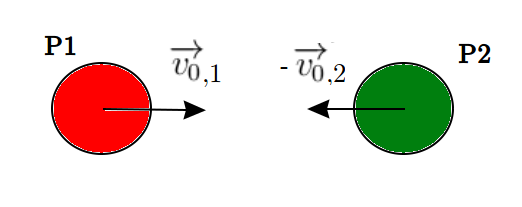
\includegraphics[width=0.45\textwidth]{chapitres/chapitre_3/figures/same-radius_same-mass.png}
    \caption{Configuration de collision 1.}\label{conf1}
\end{figure}

\begin{itemize}
    \item Vitesse initiale de la particule 1 avant le choc:\\
    $v_{0,1} = 0.149200765298 \quad m.s^{-1} $ 
    \item Vitesse initiale de la particule 2 avant le choc:\\
    $v_{0,2} = -0.149200765298 \quad m.s^{-1} $
\end{itemize}

\begin{center}
\begin{table}[!h]
\begin{tabular}{ |p{5.75cm}|p{6.8cm}| }

 \hline \rowcolor{lightgray}
 Pas de temps & Erreur absolue\\
 \hline
 $\Delta t = 1\times10^{-4}$ & $err_{abs} = 0.27142177\times10^{-12}$\\
 $\Delta t = 2.5\times10^{-4}$ & $err_{abs} = 0.54281579\times10^{-12}$\\
 $\Delta t = 5\times10^{-4}$ & $err_{abs} = 0.10856038\times10^{-11}$\\
 $\Delta t = 1\times10^{-3}$ & $err_{abs} = 0.21711799\times10^{-11}$\\
 $\Delta t = 5\times10^{-3}$ & $err_{abs} = 0.86846363\times10^{-11}$\\
 \hline
\end{tabular}
\caption{Erreur absolue de la vitesse après le choc en fonction du pas de temps (configuration de collision 1).}\label{tab2}
\end{table}
\end{center}

D'après la Table \ref{tab2}, l'erreur absolue entre la vitesse analytique et la vitesse numérique obtenue par PDAS après le choc est nulle, la quantité de mouvement avant et après choc est alors conservée pour la configuration 1. 

\subsubsection{Masses et rayons identiques, vitesses différents}

\begin{center}
\begin{table}[!h]
\begin{tabular}{ |p{5.75cm}|p{6.8cm}| }
 \hline  \rowcolor{lightgray}

 Paramètre& Valeur\\
 \hline
 Rayons Particules 1 et 2  ($m$) & $r_1 = r_2 = 2\times10^{-2}$\\
 Densité volumique ($Kg.m^{-3}$)& $\rho = 2600$\\
 Positions initiales ($m$) & $x_{0,1} \neq x_{0,2}, \quad y_{0,1} = y_{0,2}$\\
 Vitesses initiales  ($m.s^{-1}$)  &$v_{0,1} \neq -v_{0,2} \quad (prises\ al\acute{e}atoirement)$\\
 Durée d'un pas de temps ($s$)&   $\Delta t = variable$\\
 Coefficient de restitution normal& $e_n = 1.0$\\
 Force de gravité ($m.s^{-2}$)& $g = 0$\\
 Paramètre schéma temporel & $\theta = 0.5$\\
 Paramètre Active Set normal &$\gamma_n = 10$\\
 Temps de collision ($s$)& $T_{choc} = 1.0268$\\
 \hline
\end{tabular}
\caption{Paramétrage de la configuration de collision 2.}\label{tab3}
\end{table}
\end{center}

\begin{figure}[!h]
  \centering
    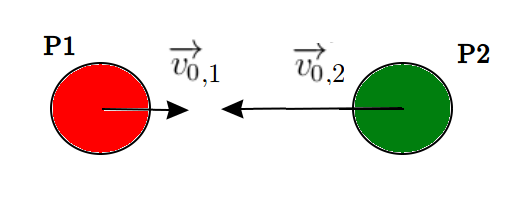
\includegraphics[width=0.45\textwidth]{chapitres/chapitre_3/figures/same-radius_same-mass_diff-vel.png}
    \caption{Configuration de collision 2.}\label{conf2}
\end{figure}

\begin{itemize}
    \item Vitesse initiale aléatoire de la particule 1 avant le choc:\\ $v_{0,1} = 0.209767707544 \quad m.s^{-1} $ 
    \item Vitesse initiale aléatoire de la particule 2 avant le choc:\\ $v_{0,2} = -0.723377058311 \quad m.s^{-1} $
\end{itemize}

\begin{center}
\begin{table}[!h]
\begin{tabular}{ |p{2.7cm}|p{4.9cm}|p{4.9cm}| }

 \hline  \rowcolor{lightgray}
 Pas de temps & Erreur absolue vitesse après choc (P1) & Erreur absolue vitesse après choc (P2)\\
 \hline
 $\Delta t = 1\times10^{-4}$ & $err_{abs} = 0.21216362\times10^{-12}$ & $err_{abs} = 0.21221913\times10^{-12}$\\
 $\Delta t = 2.5\times10^{-4}$ & $err_{abs} = 0.42432724\times10^{-12}$ & $err_{abs} = 0.42438275\times10^{-12}$\\
 $\Delta t = 5\times10^{-4}$ & $err_{abs} = 0.84865448\times10^{-12}$ & $err_{abs} = 0.84873775\times10^{-12}$\\
 $\Delta t = 1\times10^{-3}$ & $err_{abs} = 0.16973090\times10^{-11}$ & $err_{abs} = 0.16974200\times10^{-11}$\\
 $\Delta t = 5\times10^{-3}$ & $err_{abs} = 0.13579027\times10^{-10}$ & $err_{abs} = 0.13579082\times10^{-10}$\\
 \hline
\end{tabular}
\caption{Erreur absolue de la vitesse après le choc en fonction du pas de temps (configuration de collision 2).}\label{tab4}
\end{table}
\end{center}

Là encore, l'erreur absolue entre la vitesse analytique et la vitesse numérique obtenue par PDAS après le choc est nulle, ce qui permet d'affirmer que la quantité de mouvement avant et après choc est également conservée pour la configuration 2 (voir Table \ref{tab4}). 

\subsubsection{Masses, rayons et vitesses différents}
\begin{center}
\begin{table}[!h]
\begin{tabular}{ |p{5.75cm}|p{6.8cm}| }
 \hline \rowcolor{lightgray}
 \hline
 Paramètre& Valeur\\
 \hline
 Rayon Particule 1  ($m$) & $r_1 = 1\times10^{-1}$\\
 Rayon Particule 2 ($m$)  & $r_2 = 4\times10^{-2}$\\
 Densité volumique ($Kg.m^{-3}$)& $\rho = 2600$\\
 Positions initiales ($m$) & $x_{0,1} \neq x_{0,2}, \quad y_{0,1} = y_{0,2}$\\
 Vitesses initiales  ($m.s^{-1}$)  &$v_{0,1} = -v_{0,2} \quad (prises\ al\acute{e}atoirement)$\\
 Durée d'un pas de temps ($s$)&   $\Delta t = variable$\\
 Coefficient de restitution normal& $e_n = 1.0$\\
 Force de gravité ($m.s^{-2}$)& $g = 0$\\
 Paramètre schéma temporel & $\theta = 0.5$\\
 Paramètre Active Set normal &$\gamma_n = 10$\\
 Temps de collision ($s$)& $T_{choc} = 0.368$\\
 \hline
\end{tabular}
\caption{Paramétrage de la configuration de collision 3.}
\end{table}
\end{center}
\vspace{-1.2cm}
\begin{figure}[!h]
  \centering
    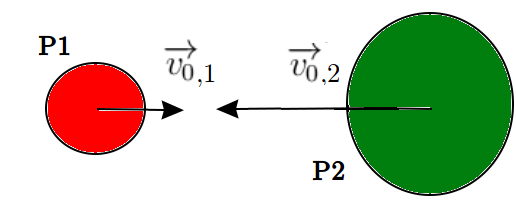
\includegraphics[width=0.45\textwidth]{chapitres/chapitre_3/figures/diff-radius_diff-mass_diff-vel.png}
    \caption{Configuration de collision 3.}\label{conf3}
\end{figure}

\begin{itemize}
    \item Vitesse initiale aléatoire de la particule 1 avant le choc:\\ $v_{0,1} = 0.691781605465 \quad m.s^{-1} $ 
    \item Vitesse initiale aléatoire de la particule 2 avant le choc:\\ $v_{0,2} = -0.997709447376 \quad m.s^{-1} $
\end{itemize}

 \begin{center}
 \begin{table}[!h]
\begin{tabular}{ |p{2.7cm}|p{4.9cm}|p{4.9cm}| }
 \hline \rowcolor{lightgray}
 Pas de temps & Erreur absolue vitesse après choc (P1) & Erreur absolue vitesse après choc (P2)\\
 \hline
 $\Delta t = 1\times10^{-4}$ & $err_{abs} = 0.55877525\times10^{-12}$ & $err_{abs} = 0.51070259\times10^{-12}$\\
 $\Delta t = 2.5\times10^{-4}$ & $err_{abs} = 0.57864824\times10^{-12}$ & $err_{abs} = 0.38635761\times10^{-12}$\\
 $\Delta t = 5\times10^{-4}$ & $err_{abs} = 0.60518257\times10^{-12}$ & $err_{abs} = 0.22071234\times10^{-12}$\\
 $\Delta t = 1\times10^{-3}$ & $err_{abs} = 0.65814021\times10^{-12}$ & $err_{abs} = 0.11057821\times10^{-12}$\\
 $\Delta t = 5\times10^{-3}$ & $err_{abs} = 0.97599706\times10^{-12}$ & $err_{abs} = 0.20974333\times10^{-11}$\\
 \hline
\end{tabular}
\caption{Erreur absolue de la vitesse après le choc en fonction du pas de temps (configuration de collision 3).}\label{tab6}
\end{table}
\end{center}
\vspace{-0.8cm}
L'état des particules P1 et P2 ne change pas, le choc est élastique et l'énergie cinétique du système est conservée pour $e_n = 1.0$. Le graphe de la Figure \ref{fig4} montre que l'énergie cinétique obtenue par la méthode PDAS ne varie pas au moment du choc. En revanche, une partie de l'énergie cinétique du système est dissipée lors du premier choc pour un coefficient de restitution $e_n = 0.5$. La somme des énergies internes de chacune des deux particules et de leur énergies potentielles d’interaction augmente car l’énergie interne du système est conservée. La quantité de mouvement reste en revanche toujours conservée.

\begin{figure}[!h]
  \centering
    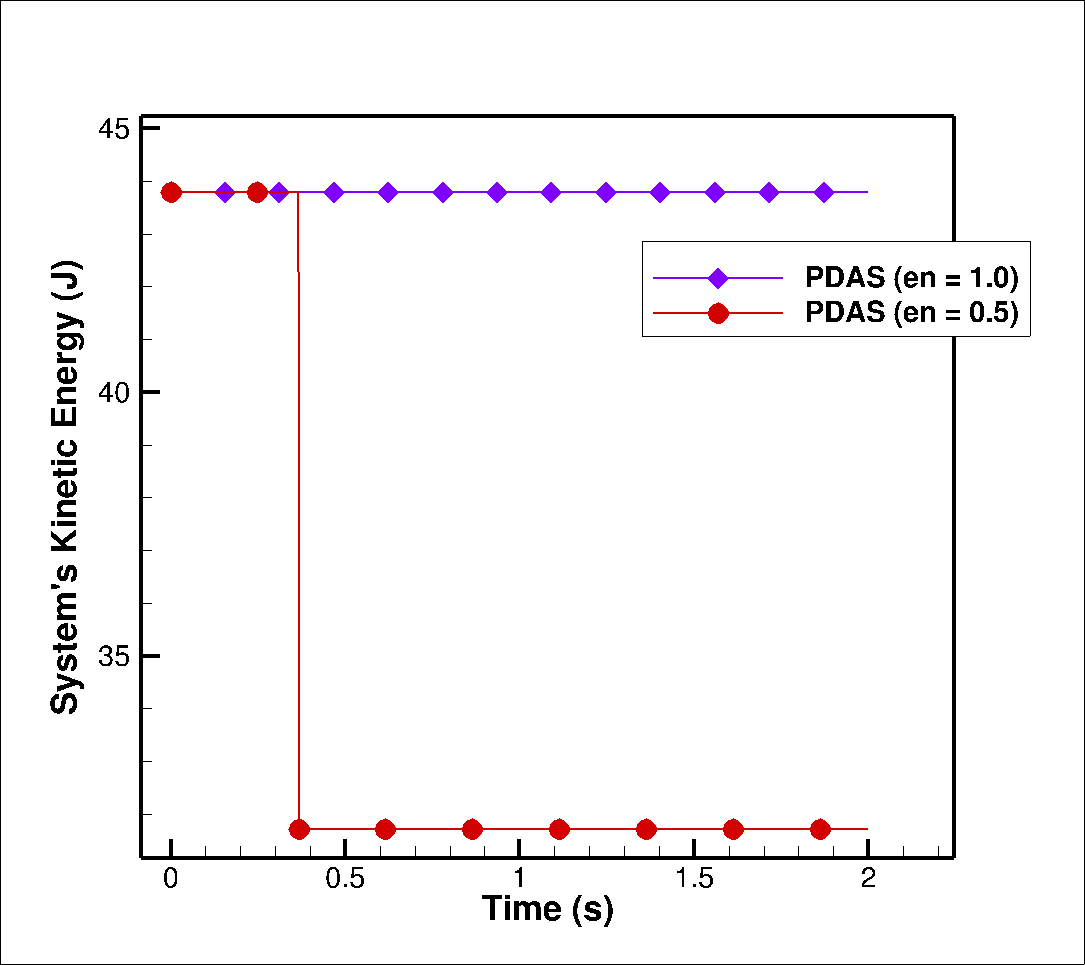
\includegraphics[width=0.6\textwidth]{chapitres/chapitre_3/figures/ec_en.png}
    \caption{\centering Évolution de l'énergie cinétique de la configuration de collision 3 obtenue par PDAS en fonction du temps pour $2$ coefficients $e_n$ distincts.}\label{fig4}
\end{figure}

\begin{center}
\begin{table}[!h]
\begin{tabular}{ |p{3cm}|p{3cm}|p{3cm}|p{2.75cm}| }
 \hline \rowcolor{lightgray}

 \centering Coefficient de restitution normal & \centering Énergie cinétique avant choc & \centering Énergie cinétique après choc & Erreur absolue\\
 \hline
 $e_n = 1.0$ & $43.7809913086674$ & $43.7809913086628$ & $4.6\times10^{-12} $\\
 $e_n = 0.5$ & $43.7809913086674$ & $31.7215198444011$ & $-$\\
 
 \hline
\end{tabular}
\caption{Évolution de l'énergie cinétique au cours du temps de la configuration de collision 3 obtenue par PDAS.}
\end{table}
\end{center}

\subsection{Chute libre d'une particule}

\subsubsection{Description du cas-test}

On se donne comme deuxième cas-test de validation celui d'une particule rigide P en chute libre, lâchée sans vitesse initiale ($V_0 = 0$), d'une hauteur initiale $h_0$, et soumise uniquement à la force de gravité $g$. La particule rebondit au moment de l'impact avec une fondation rigide fixe. Le mouvement de translation de la particule est décrit en trois étapes, comme le montre la Figure \ref{fig35}: Chute libre, Contact et Rebond. Une expression analytique du mouvement des particules à chaque étape peut être déterminée.

\begin{figure}[!h]
  \centering
    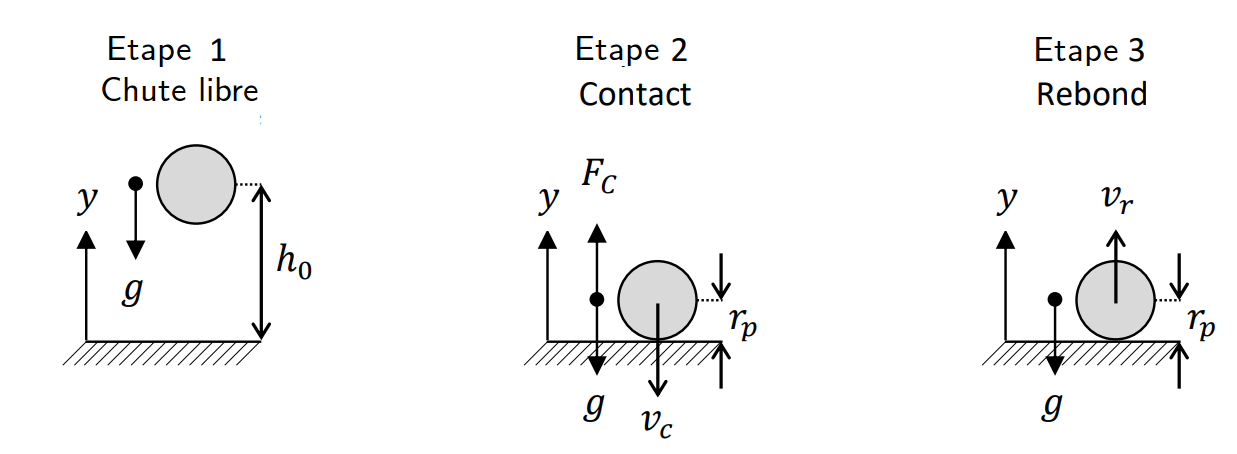
\includegraphics[width=0.9\textwidth]{chapitres/chapitre_3/figures/free_fall.png}
    \caption{Chute libre d'une particule rigide P sans vitesse initiale, soumise uniquement à la force de gravité.}\label{fig35}
\end{figure}

La particule de rayon $r_p$ tombe sur la fondation fixe, puis rebondit sous l'effet de la force de collision répulsive particule-paroi $F_c$, $v_c$ étant la vitesse de la particule avant la collision, et $v_r$ sa vitesse après la collision.

\subsubsection{Solution analytique du problème}

A l'instant initial ($t = t_0 = 0$), un équilibre des forces sur la particule fournit une expression de son mouvement pendant la chute libre

\begin{equation}
    \frac{d^2 y}{dt^2} = -g; \quad y(0) = h_0; \quad \frac{dy}{dt}(0) = 0
\end{equation}

où $y$ est la position centrale de la particule par rapport à la paroi et $g$ est l'accélération due à la gravité. La particule est initialement au repos à une hauteur $h_0$ au-dessus du mur. La vitesse instantanée, $v$, et la position centrale de la particule P sont données par: 

\begin{equation}
    v(t) = -gt \label{vt}
\end{equation}

\begin{equation}
    y(t) = h_0 - \frac{1}{2}gt^2 \label{yt}
\end{equation}

A l'instant de contact ($t = t_c$), l'étape de chute libre se termine et l'étape de contact commence lorsque la position centrale de la particule P est égale à son rayon $r_p$. Le contact est exprimé en déplacement et la vitesse initiale de P est obtenue en combinant (\ref{vt}) et (\ref{yt}) lorsque sa position centrale y est égale à son rayon $r_p$.

L'étape de contact se termine et l'étape de rebond commence lorsque la position centrale de P est à nouveau égale à son rayon. Un équilibre des forces sur la particule conduit à une expression du mouvement des particules comme suit:

\begin{equation}
    \frac{d^2 y}{dt^2} = -g(t); \quad y(t_c) = r_p; \quad \frac{dy}{dt}(t_c) = - v_c
\end{equation}

Du fait de la discontinuité de la vitesse avant et après le choc, la vitesse au début de la phase de rebond est égale à l'opposé de la vitesse à la fin de la phase de contact, $v_c$. La vitesse instantané, $v$, et la position centrale de P, $y$, sont données par:

\begin{equation}
    v(t) = - v_c - g(t-t_c)
\end{equation}

\begin{equation}
    y(t) = r_p - v_c(t-t_c) - \frac{1}{2}g(t-t_c)^2
\end{equation}

Après le rebond, la vitesse après choc est quantifiée grâce au coefficient de restitution $e_n$ mis en jeu, et qui dépend des caractéristiques physique de la particule. Nous allons donc vérifier l'exactitude de cette vitesse après choc pour différents coefficient de restitution en comparant les résultats obtenus par PDAS avec les solutions analytiques du problème.
    
\subsubsection{Paramétrage du cas-test}

La Table ci-dessous reprend les différents paramètres physiques et numériques pour la réalisation de ce cas-test:

\begin{center}
\begin{table}[!h]
\begin{tabular}{ |p{5.75cm}|p{6.8cm}| }
 \hline \rowcolor{lightgray}
 Paramètre& Valeur\\
 \hline
 Rayon particule P  ($m$) & $r_p = 2\times10^{-2}$\\
 Densité volumique ($Kg.m^{-3}$)& $\rho = 2600$\\
 Hauteur initiale ($m$) & $h_0 = 0.5$\\
 Vitesse initiale  ($m.s^{-1}$)  &$v_0 = 0$\\
 Durée d'un pas de temps ($s$)&   $\Delta t = 1.55\times10^{-4}$\\
 Nombre de pas de temps& $N_{time\ steps} = 10000$\\
 Coefficient de restitution normal & $e_n = variable$\\
 Force de gravité ($m.s^{-2}$)& $g = -9.80665$\\
 Masse de la particule ($Kg$)  &$m_1 = \rho \pi r_1^{2}$\\
 Paramètre schéma temporel & $\theta = 0.5$\\
 Paramètre Active Set normal &$\gamma_n = 10$\\
 Temps de collision ($s$)& $T_{choc} = 0.313$\\
 \hline
\end{tabular}
\caption{Paramétrage de la configuration de chute d'une particule.}
\end{table}
\end{center}
    
\subsubsection{Résultats numériques}    

La simulation, d'une durée totale de $T = 1.55 s$, permet de vérifier la validité de la méthode numérique PDAS, en comparant les résultats numériques ainsi obtenus des positions et vitesses de la particule P en chute libre avec les solutions analytiques, et ce, pour différents coefficients de restitution. 
    \begin{figure}[!h]
  \centering
    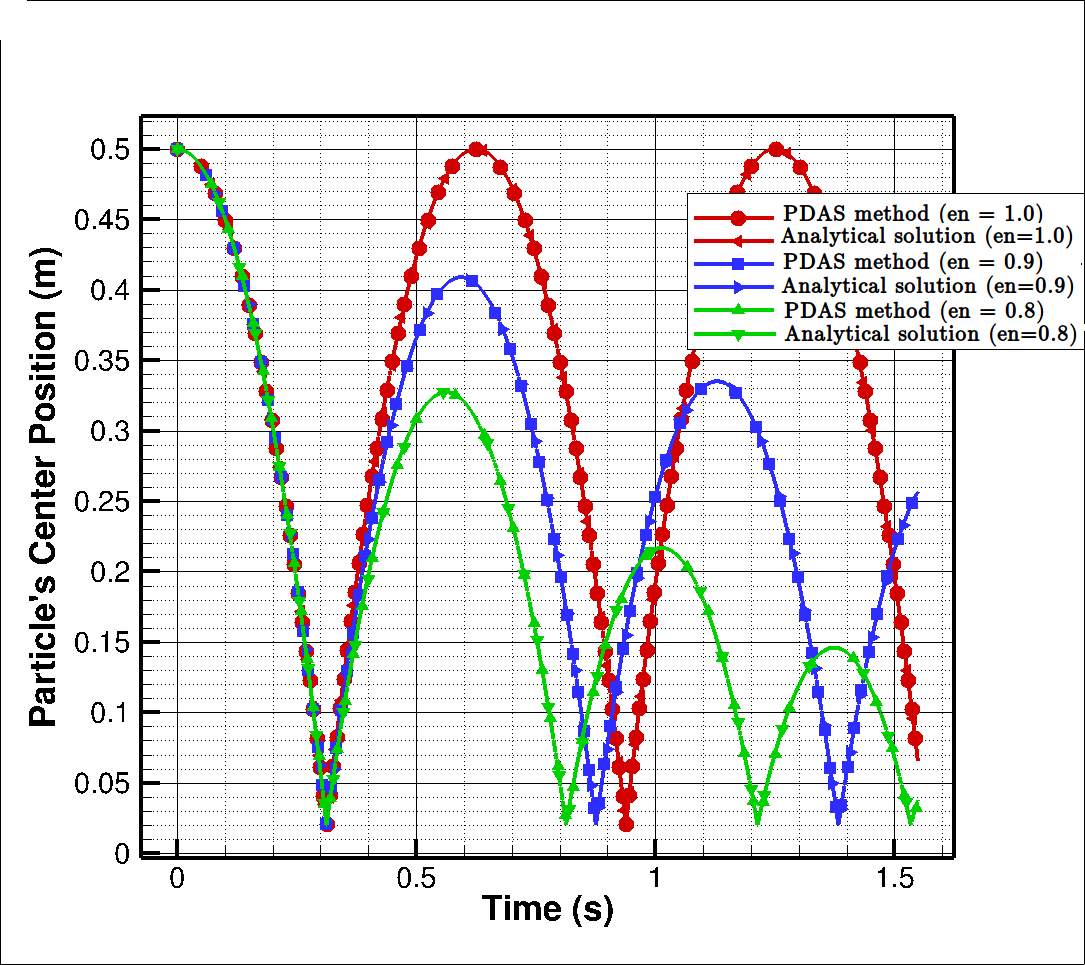
\includegraphics[width=0.6\textwidth]{chapitres/chapitre_3/figures/x_it_free_falling_particule_en=varied_AS(AM)_vs_anal_sol.png}
    \caption{\centering Comparaison de la solution analytique et des résultats numériques de la position d'une particule P en chute libre obtenus par PDAS pour différents coefficients de restitution $e_n$.}\label{fig36}
\end{figure}
    
    \vspace{1cm}
    
\begin{figure}[!h]
  \centering
    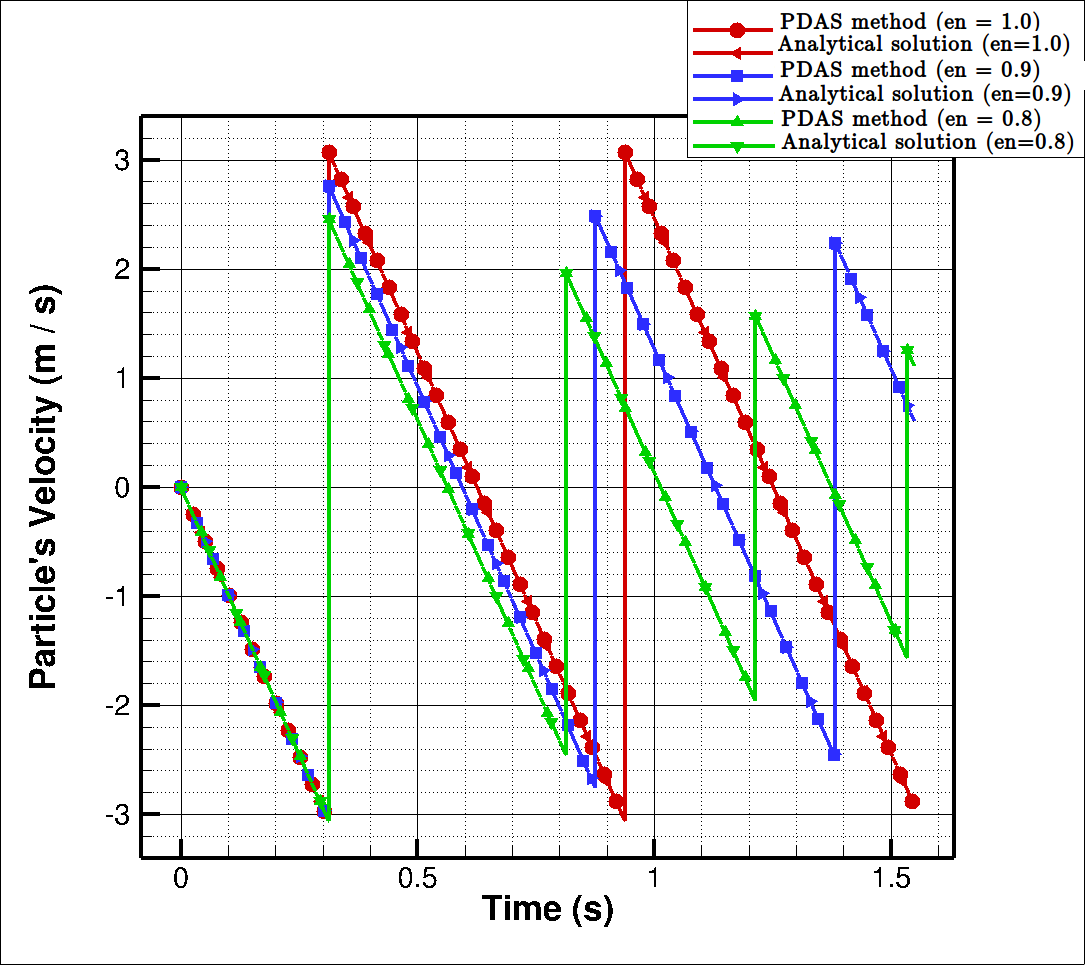
\includegraphics[width=0.6\textwidth]{chapitres/chapitre_3/figures/vel_it_free_falling_particule_en=varied_AS(AM)_vs_anal_sol.png}
    \caption{\centering Comparaison de la solution analytique et des résultats numériques de la vitesse d'une particule P en chute libre obtenus par PDAS pour différents coefficients de restitution $e_n$.}\label{fig37}
\end{figure}
    
D'après les graphes des Figures \ref{fig36} et \ref{fig37}, la particule P revient à sa hauteur initiale après chaque rebond, et va vitesse avant le choc est égale à celle après le choc en valeur absolue pour un coefficient de restitution $e_n = 1.0$. De plus, les variations numériques de la position et de la vitesse au cours du temps sont identiques à celles de la solution analytique pour les différents coefficients de restitution $[e_n = 1.0, 0.9, 0.8]$. D'autre part, la courbe rouge de la Figure \ref{fig38} présente la tendance de variation de l'énergie cinétique du système pour un coefficient de restitution $e_n = 1.0$, qui atteint la même valeur maximale après chaque rebond. L'énergie cinétique du système est alors conservée. 
    
\begin{figure}[!h]
  \centering
    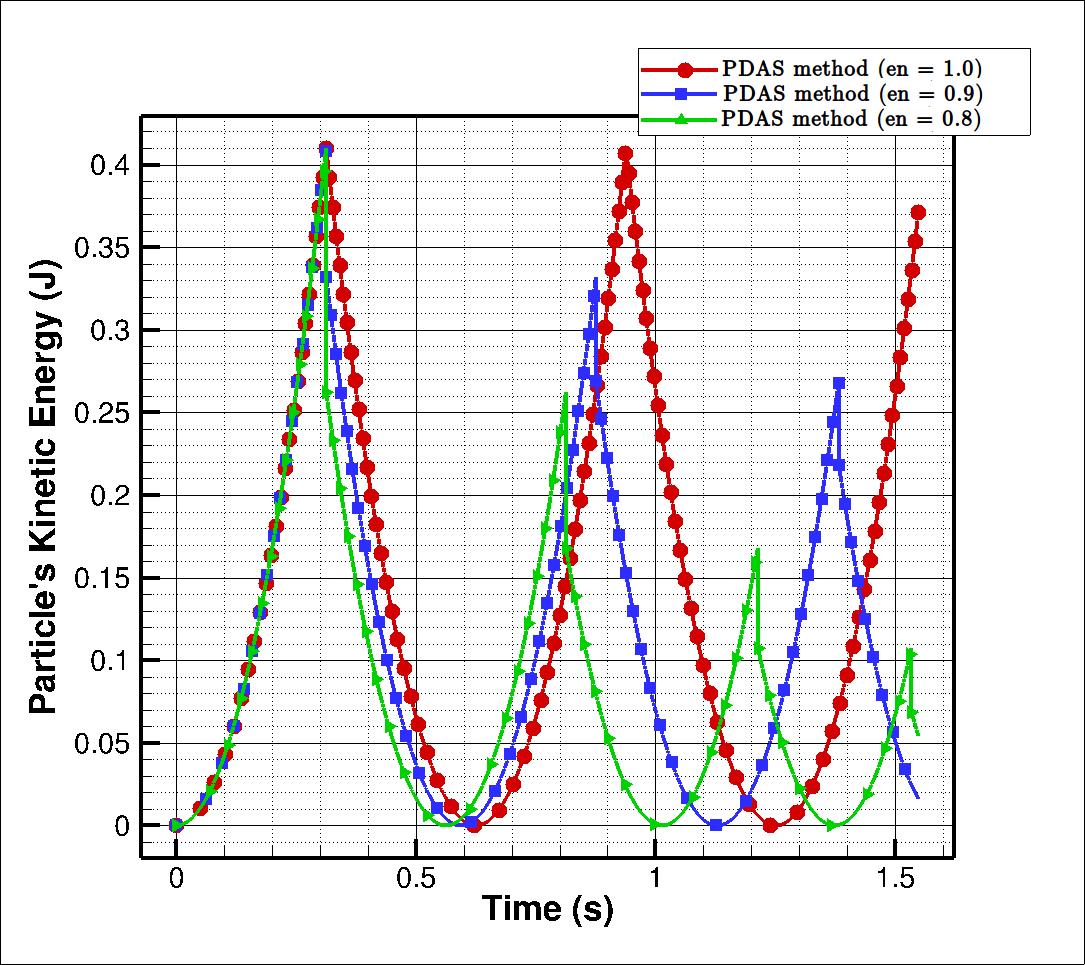
\includegraphics[width=0.6\textwidth]{chapitres/chapitre_3/figures/ec_it_free_falling_particule_en=varied_AS(AM).png}
    \caption{\centering Évolution de l'énergie cinétique obtenue par PDAS au cours du temps d'une particule P en chute libre pour différents coefficients de restitution $e_n$.}\label{fig38}
\end{figure}

Par ailleurs, une étude comparative entre la solution numérique obtenue par PDAS et celles obtenues par Lagrangien augmenté standard et bi-potentiel amélioré est réalisée pour ce cas-test. 

\begin{figure}[!h]
  \centering
    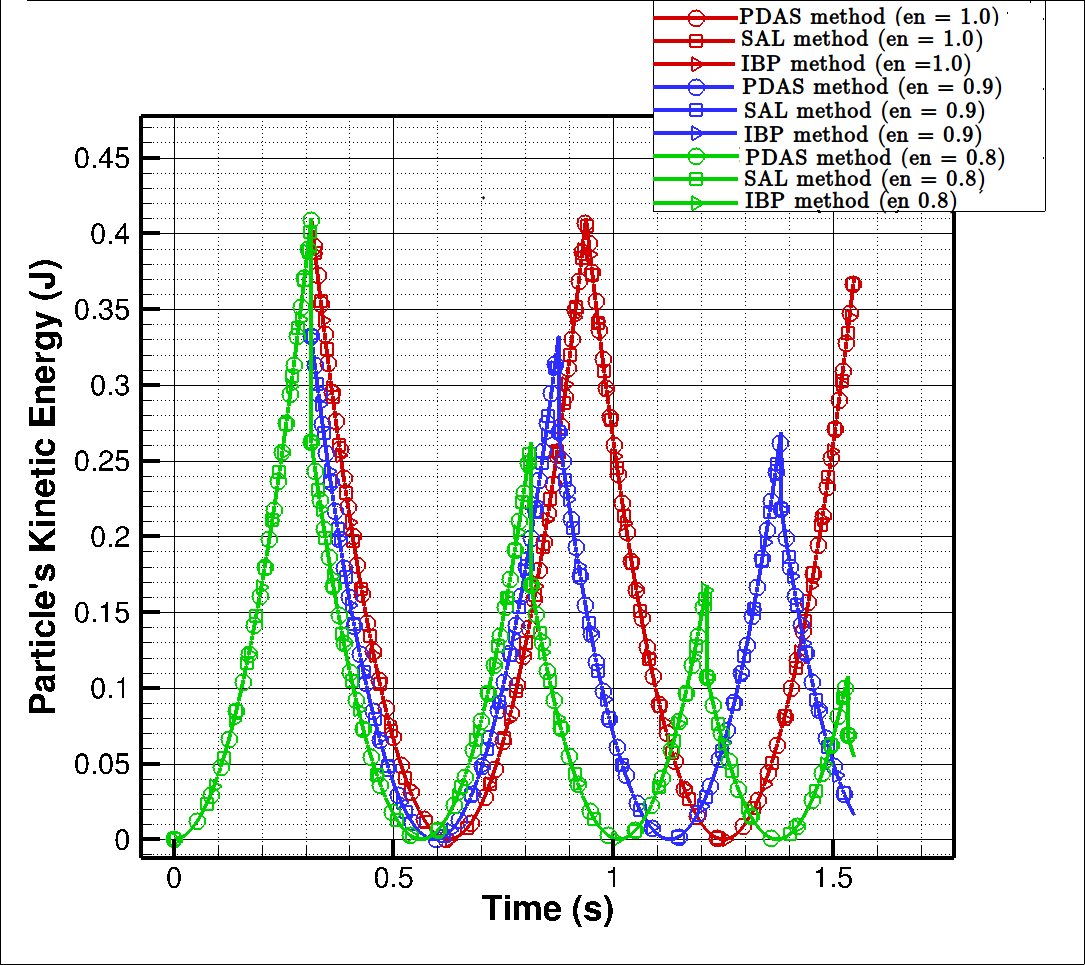
\includegraphics[width=0.6\textwidth]{chapitres/chapitre_3/figures/ec_it_free_falling_particule_en=varied_AS(AM)_vs_LG_vs_BP.png}
    \caption{\centering Comparaison de l'évolution de l'énergie cinétique obtenus par PDAS au cours du temps d'une particule P en chute libre pour différentes méthodes numériques et différents coefficients de restitution $e_n$.}\label{fig39}
\end{figure}


\begin{figure}[!h]
  \centering
    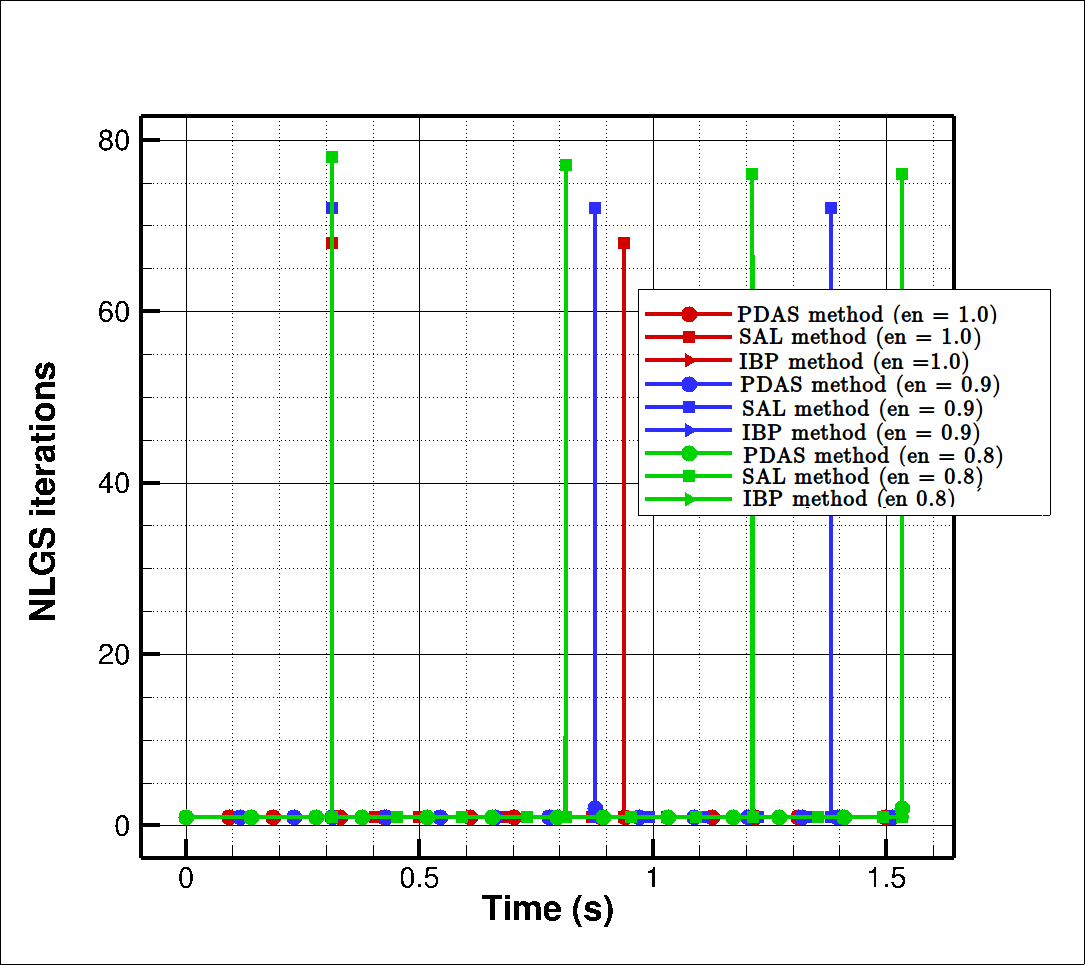
\includegraphics[width=0.6\textwidth]{chapitres/chapitre_3/figures/nlgs_it_free_falling_particule_en=varied_AS(AM)_vs_LG_vs_BP.png}
    \caption{\centering Comparaison du nombre d'itérations NLGS obtenus par PDAS, SAL et IBP au cours du temps d'une particule P en chute libre pour différents coefficients de restitution $e_n$.}\label{fig310}
\end{figure}

La Figure \ref{fig39} montre que la variation d'énergie cinétique au cours du temps obtenue par les 3 méthodes numériques est identique suivant le coefficient de restitution. Quant à l'évolution des itérations non-linéaires NLGS au cours du temps, la Figure \ref{fig310}, montre que, indépendamment du coefficient de restitution, les méthodes PDAS et IBP convergent plus rapidement ($1$ itération NLGS représentées par les symboles $\bullet$ et $\blacktriangleright$) au moment du choc que la méthode SAL (entre $68$ et $78$ itérations NLGS représenté sur le graphe par les pics en symbole $\blacksquare$).

Ainsi, les courbes ci-dessus confirment la validité de l'approche numérique PDAS sans frottement pour ce cas-test.

\subsection{Problème d'équilibre}

\subsubsection{Description du cas-test}

On traite à présent un troisième cas-test de validation où l'on considère 5 particules rigides empilées les unes sur les autres en équilibre et sans frottement (voir Figure \ref{fig311}) . Les particules, de rayons et de masses identiques, ont des vitesses initiales nulles, et sont soumises uniquement à l'action de la force de gravité. Il s'agit à travers ce problème académique, de déterminer numériquement les impulsions de contact obtenues par PDAS et de les comparer à la solution analytique. 

\begin{figure}[!h]
  \centering
    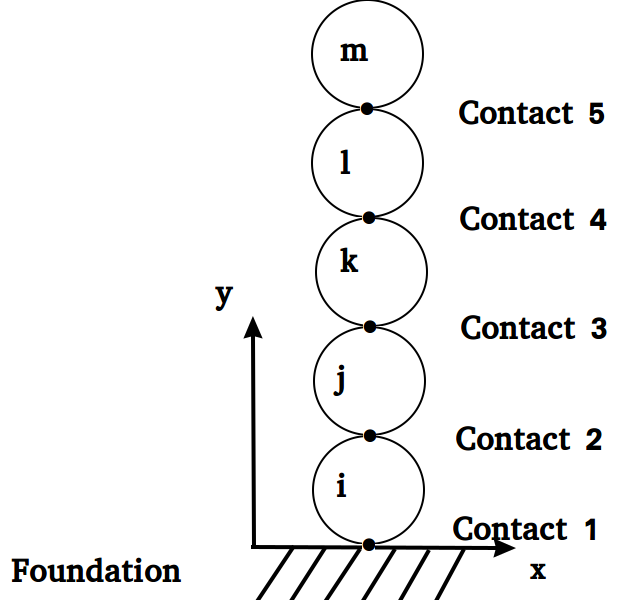
\includegraphics[width=0.45\textwidth]{chapitres/chapitre_3/figures/5_stacked_particles.png}
    \caption{Colonne de 5 particules en 2D empilées les unes sur les autres en équilibre.}\label{fig311}
\end{figure}

Pour ce faire, nous utilisons les paramètres physiques et numériques décrits dans la Table ci-dessous:

\begin{center}
\begin{table}[!h]
\begin{tabular}{ |p{5.75cm}|p{6.8cm}| }
 \hline \rowcolor{lightgray}

 Paramètre& Valeur\\
 \hline
 Rayons des particules ($m$) & $r_n = 2\times10^{-2}; \quad n = i,j,k,l,m$\\
 Densité volumique ($Kg.m^{-3}$)& $\rho = 2600$\\
 Vitesses initiales ($m.s^{-1}$)  &$v_{0,n} = 0; \quad n = i,j,k,l,m$\\
 Durée d'un pas de temps ($s$)&   $\Delta t = 1\times10^{-3}$\\
 Nombre de pas de temps& $N_{Time\ steps} = 1000$\\
 Coefficient de restitution normal& $e_n = 1.0$\\
 Force de gravité ($m.s^{-2}$)& $g = -9.80665$\\
 Masse des particules ($Kg$)  &$m_n = \rho \pi r_n^{2}; \quad n = i,j,k,l,m$\\
 Paramètre schéma temporel & $\theta = 0.5$\\
 Paramètre Active Set normal &$\gamma_n = 10$\\
 \hline
\end{tabular}
\caption{Paramétrage de la configuration d'équilibre.}
\end{table}
\end{center}
    
\subsubsection{Solution analytique du problème}    
    
Théoriquement, le principe fondamental de la dynamique permet de déterminer les impulsions de chaque contact du système $S$ représenté sur la Figure \ref{fig311}:

\begin{equation}\label{pfd}
    \sum{\textbf{F{ext}}} = m_n\textbf{a}
\end{equation}
 
 En isolant la particule $m$ et en appliquant (\ref{pfd}) sur le système isolé $S \setminus{[i,j,k,l]}$, 
 \begin{equation}
    \textbf{R}_{l,m} = m_mg_y\textbf{y}
 \end{equation}

où $\textbf{R}_{l,m}$ représente la réaction de la particule $l$ sur la particule $m$, soit l'impulsion du contact 5, $m_m$ la masse de la particule m et $g_y$ la composante en $y$ de la gravité.
On isole maintenant le système $S \setminus{[i,j,k]}$ constitué des particules $m$ et $l$ et on applique (\ref{pfd}),

\begin{equation}
    \textbf{R}_{k,l} + \textbf{R}_{m,l} = m_lg_y\textbf{y}
\end{equation}
 sachant que $\textbf{R}_{m,l} = - \textbf{R}_{l,m}$ et que $m_l = m_m$, on obtient:
 
 \begin{equation}
    \textbf{R}_{k,l} = 2m_lg_y\textbf{y}
\end{equation}
 En procédant de façon itérative, on obtient la solution analytique du problème d'équilibre:
 
 \begin{center}
 \begin{table}[!h]
\begin{tabular}{ |p{5.3cm}|p{7.2cm}| }
 \hline \rowcolor{lightgray}

 Contact& Valeur théorique de l'impulsion de contact\\
 \hline
 Contact 5 ($N.s$) & $r_{c5} = m_ng_y$\\
 Contact 4 ($N.s$) & $r_{c4} = 2m_ng_y$\\
 Contact 3 ($N.s$) & $r_{c3} = 3m_ng_y \quad n = i,j,k,l,m$\\
 Contact 2 ($N.s$) & $r_{c2} = 4m_ng_y$\\
 Contact 1 ($N.s$) & $r_{c1} = 5m_ng_y$\\
 \hline
\end{tabular}
\caption{Solutions analytiques des impulsions de contact pour tous les contacts de la configuration d'équilibre.}
\end{table}
\end{center}

\subsubsection{Résultats numériques}

Les résultats numériques obtenus par PDAS pour ce problème d'équilibre avec les paramètres physiques et numériques décrits précédemment sont cohérents avec la théorie. En effet, si l'on considère par exemple le contact 5, $m_n = m_l = \rho \pi r_n^{2} \approx 3.267 \quad Kg$,  $g_y = 9.80665 \quad m.s^{-2}$, le produit $m_ng_y$ correspond à la valeur numérique de $r_{c5}$.

\begin{center}
\begin{table}[!h]
\begin{tabular}{ |p{5.75cm}|p{6.8cm}| }
 \hline \rowcolor{lightgray}
 Contact& Erreur relative (\%)\\
 \hline
 Contact 5 ($N.s$) & $err_{c5} = 2.74\times10^{-7}$\\
 Contact 4 ($N.s$) & $err_{c4} = 2.65\times10^{-7}$\\
 Contact 3 ($N.s$) & $err_{c3} = 2.47\times10^{-7} \quad n = i,j,k,l,m$\\
 Contact 2 ($N.s$) & $err_{c2} = 2.22\times10^{-7}$\\
 Contact 1 ($N.s$) & $err_{c1} = 1.84\times10^{-7}$\\
 \hline
\end{tabular}
\caption{Erreurs relatives en pourcentage par rapport aux solutions analytiques des impulsions de contact obtenues par PDAS pour tous les contacts de la configuration d'équilibre.}
\end{table}
\end{center}

\vspace{-1.75cm}

\subsection{Particules à trajectoires et vitesses aléatoires}
\subsubsection{Description du cas-test}

On se donne comme dernier cas-test de validation un système constitué de $81$ particules se déplaçant dans une boîte bidimensionnelle, à vitesses initiales aléatoires, sans forces de gravité, sans frottement, et on se propose, d'une part, d'étudier la conservation de l'énergie cinétique du système étudié pour différents coefficients de restitution (cf. Figure \ref{fig312}), et d'autre part, de comparer la convergence des 3 méthodes (PDAS, SAL et IBP) pour ce même système.

\begin{figure*}[h!] 
    \centering
    \subfloat[]{%
        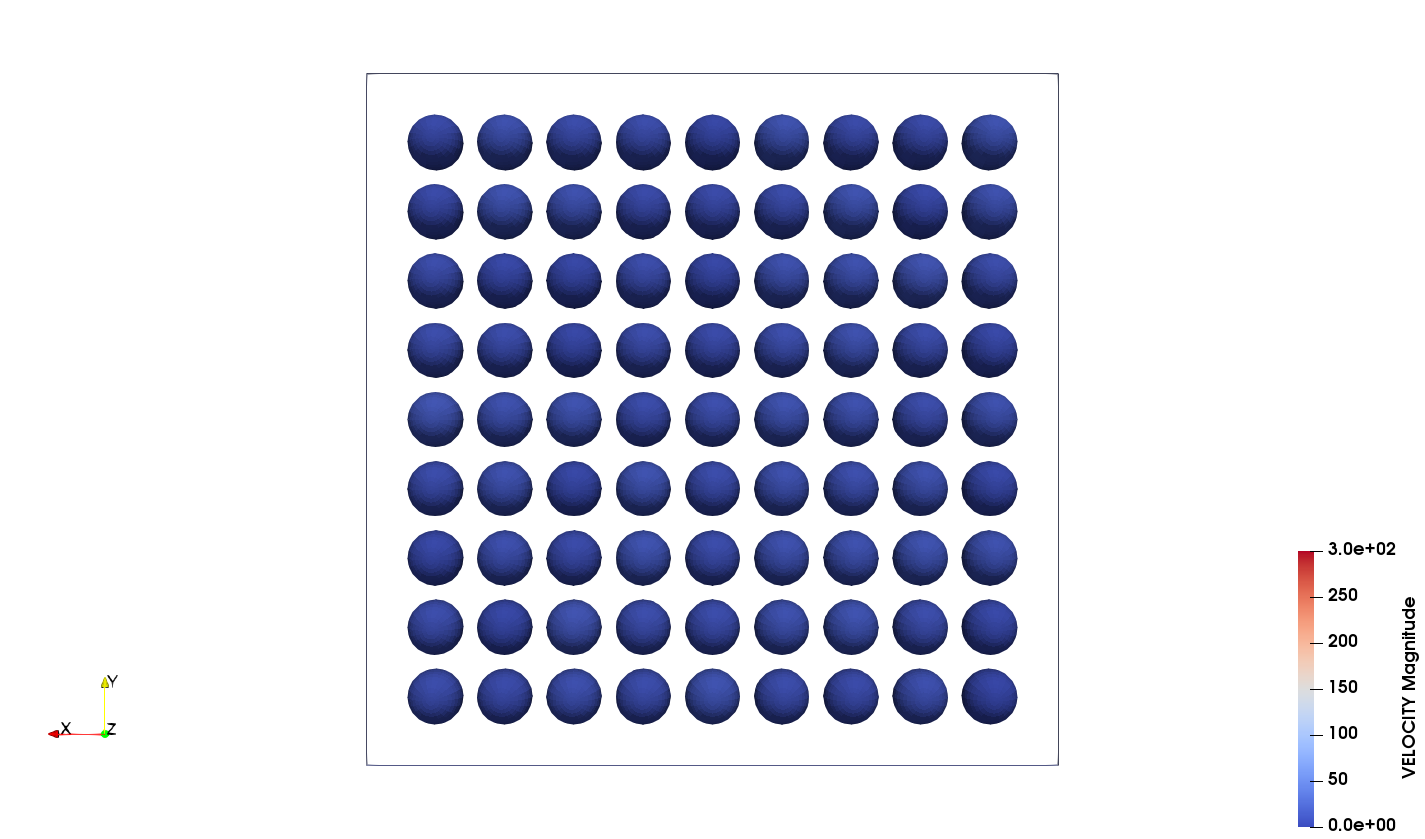
\includegraphics[width=0.5\linewidth]{chapitres/chapitre_3/figures/81_part_before_transparent.png}%
        \label{fig:81_before}%
        }%
    \hfill%
    \subfloat[]{%
        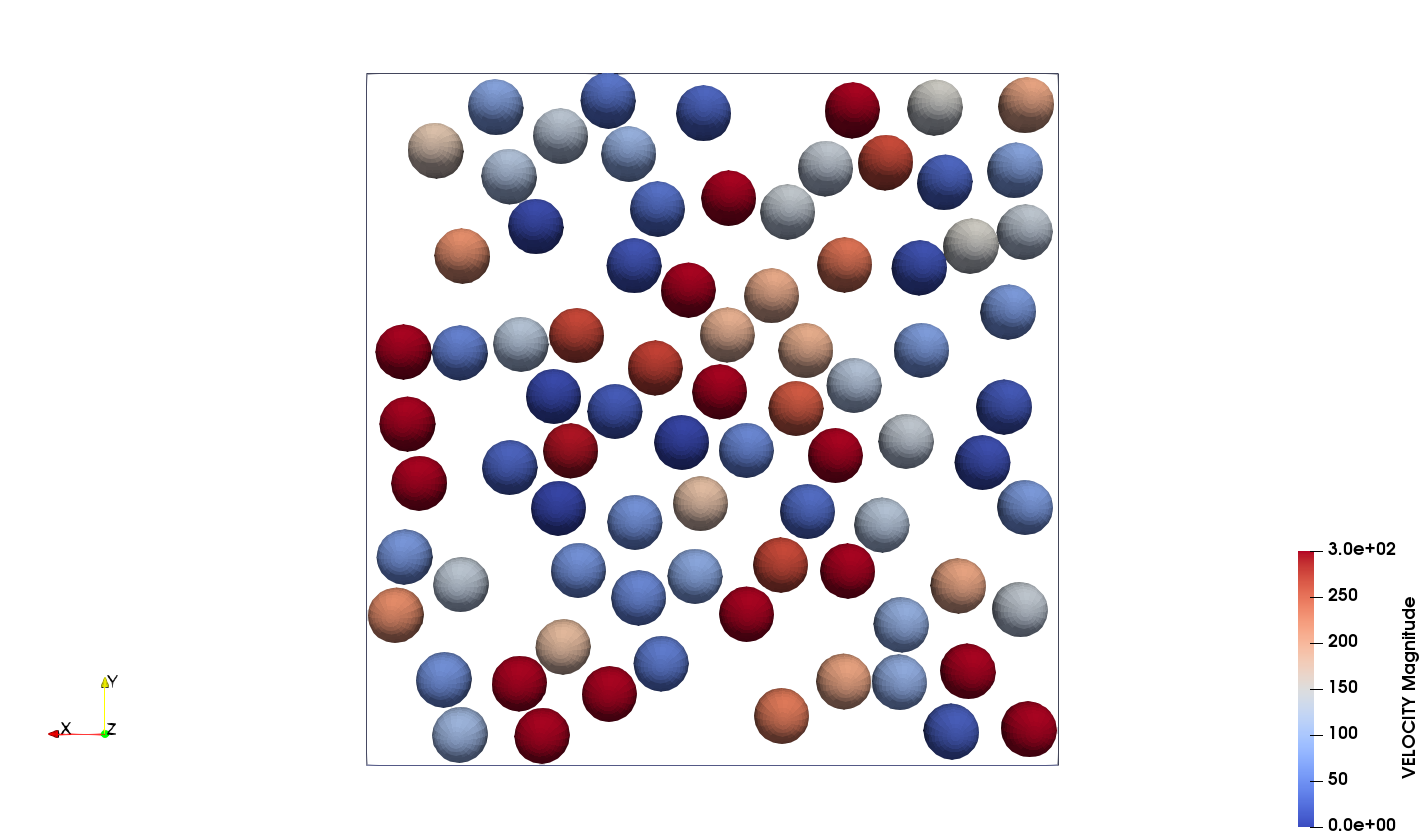
\includegraphics[width=0.5\linewidth]{chapitres/chapitre_3/figures/81_part_after_transparent.png}%
        \label{fig:81_after}%
        }%
    \caption{ $[a]$ Configuration initiale à $t = 0$ et $[b]$  configuration à $t \neq 0$ du système bidimensionnel à 81 particules à trajectoires et vitesses aléatoires au cours du temps sans frottement et sans gravité.}\label{fig312}
\end{figure*}

La Table ci-dessous reprend les différents paramètres physiques et numériques du problème étudié:

\begin{center}
\begin{table}[!h]
\begin{tabular}{ |p{5.75cm}|p{6.8cm}| }
 \hline \rowcolor{lightgray}

 Paramètre& Valeur\\
 \hline
 Nombre de particules & $n_p = 81$\\
 Rayons des particule ($m$) & $r_p = 8\times10^{-2}$\\
 Densité volumique ($Kg.m^{-3}$)& $\rho = 2600$\\
 Dimensions du domaine ($m*m$) & $[0.0,2.0] \times [0.0,2.0]$\\
 Vitesses initiales  ($m.s^{-1}$)  &$v_{0,p} = al\acute{e}atoire$\\
 Durée d'un pas de temps ($s$)&   $\Delta t = 1\times10^{-4}$\\
 Nombre de pas de temps& $N_{time\_steps} = 10000$\\
 Coefficient de restitution normal& $e_n = variable$\\
 Force de gravité ($m.s^{-2}$)& $g = 0.0$\\
 Masse des particules ($Kg$)  &$m_n = \rho  \pi r_p^{2}$\\
 Paramètre schéma temporel & $\theta = 0.5$\\
 Paramètre Active Set normal &$\gamma_n = 10$\\
 \hline
\end{tabular}
\caption{Paramétrage  de la configuration des particules à trajectoires et vitesses aléatoires.}
\end{table}
\end{center}
\vspace{-1.0cm}
\subsubsection{Résultats numériques}

La Table \ref{ec_81part} montre que la variation d'énergie cinétique du système est de l'ordre de $10^{-13}$ au fur et à mesure que le nombre de chocs augmente pour un coefficient de restitution $en = 1.0$. L'énergie cinétique du système est conservée (voir Figure \ref{fig313})

\begin{center}
\begin{table}[!h]
\begin{tabular}{ |p{5.75cm}|p{6.8cm}| }
 \hline \rowcolor{lightgray}

 Nombre de chocs& Energie cinétique du système (J)\\
 \hline
 1 & $E_c = 150.61798555315164$\\
 4 & $E_c = 150.61798555315161$\\
 16 & $E_c = 150.61798555315158$\\
 32 & $E_c = 150.61798555315167$\\
 64 & $E_c = 150.61798555315156$\\
 \hline
\end{tabular}
\caption{Évolution de l'énergie cinétique du système obtenue par PDAS en fonction du nombre de chocs.}\label{ec_81part}
\end{table}
\end{center}

\begin{figure}[!h]
  \centering
    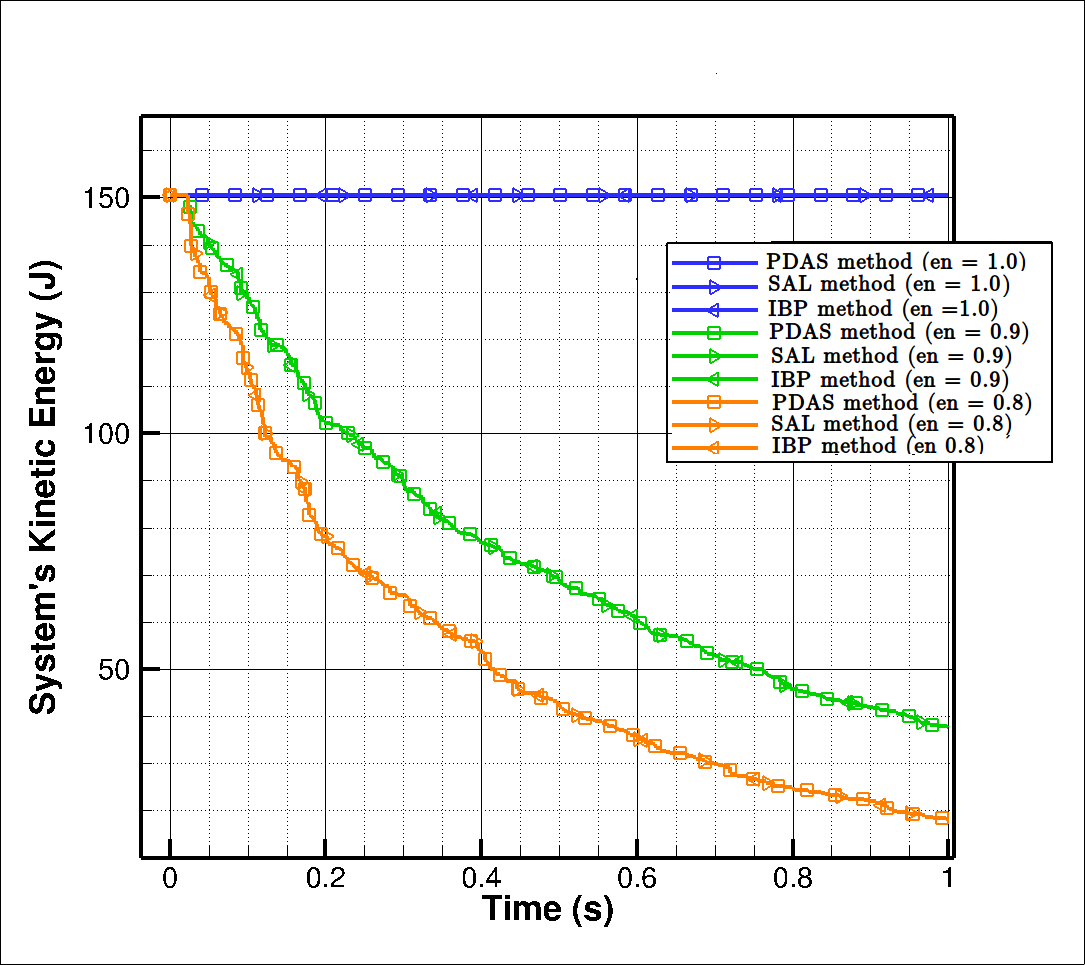
\includegraphics[width=0.5\textwidth]{chapitres/chapitre_3/figures/ec_it_81_particule_mu=0_en=varied_AS-LG-BP.png}
    \caption{Évolution de l'énergie cinétique du système au cours du temps pour différentes méthodes numériques et différents coefficients de restitution $e_n$.}\label{fig313}
\end{figure}

En ce qui concerne la convergence des méthodes numériques utilisées pour ce cas-test, un constat général se dégage d'après les courbes de la Figure \ref{fig314}. En effet, les méthodes PDAS et IBP (symboles $\blacksquare$ et $\blacktriangleleft$) convergent plus rapidement que la méthode SAL, méthode pour laquelle le nombre d'itérations NLGS cumulées dépasse les $200000$ itérations (symbole $\blacktriangleright$), et ce, pour un $e_n = 1.0$.

\begin{figure}[!h]
  \centering
    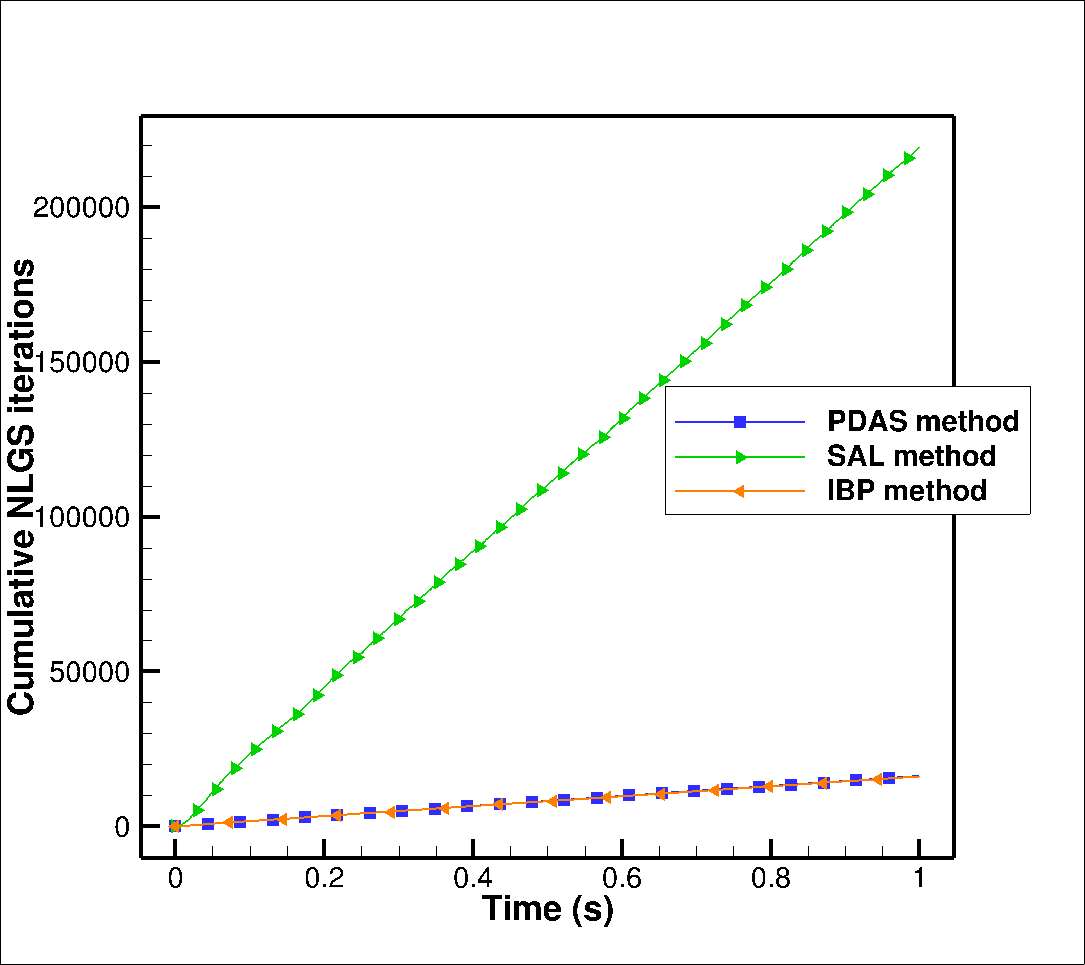
\includegraphics[width=0.5\linewidth]{chapitres/chapitre_3/figures/nlgs_it_81_particule_mu=0_en=varied_AS-LG-BP.png}%
        \label{fig:81_nlgs}%
    \caption{Évolution du nombre d'itérations NLGS au cours du temps pour différentes méthodes numériques et un coefficient de restitution $e_n = 1.0$.}\label{fig314}
\end{figure}

\newpage

\section{Cas-tests de validation: Contact avec frottement}\label{friction_test_cases}

L'objectif principal de cette section est de fournir plusieurs simulations numériques sur des cas-tests de contact avec frottement pour évaluer les méthodes PDAS dans la résolution de problèmes multi-contacts en milieu granulaire. Pour ce faire, nous considérons pour les deux premières simulations les configurations de référence suivantes: une seule bille sphérique d'acier posée sur un tapis roulant et une autre posée au fond d'un tambour fixe. Ces deux configurations permettent de vérifier d'une part, les propriétés mécaniques de base telles que la conservation de l'énergie d'un système pour les méthodes PDAS, et, d'autre part, puisque la solution analytique est disponible pour le premier cas-test, de la comparer avec la solution numérique. La deuxième partie de cette section met en lumière la robustesse et la précision des méthodes PDAS, en réalisant des simulations plus complexes comme la sédimentation d'un ensemble de billes. Les performances de calcul des méthodes PDAS sont illustrées en les comparant aux deux autres méthodes numériques SAL et IBP. La dernière simulation d'un écoulement granulaire dans un tambour rotatif 2D permet d'établir des comparaisons avec des expériences.


%------------------------------------------------------------------
\subsection{Roulement glissement d'une bille d'acier sur tapis roulant}\label{ex1}

Le but de ce cas-test est de réaliser des comparaisons entre solutions numériques et analytiques. Une bille d'acier sphérique, de vitesse horizontale initiale ($v_0 = 1m.s^{-1}$) est placée sur un tapis roulant de vitesse constante ($\vect{V_1} = v_1 \vect{x}$ avec $v_1 = 2m.s^{-1}$) comme présenté dans la Figure ci-après. Nous fournissons ci-dessous une description des paramètres physiques relatives au cas-test

\begin{figure}[h!]
	\begin{center}
		\resizebox{10cm}{!}{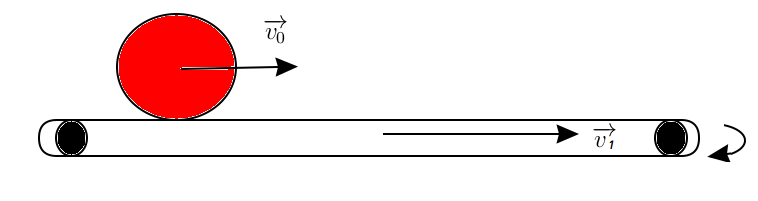
\includegraphics{chapitres/chapitre_3/figures/tapis_roulant.png}}
	\end{center}
	\caption{Roulement glissement d'une bille d'acier sur un tapis roulant.}
	\label{conv_belt}
\end{figure}

\begin{eqnarray*}
	\begin{array}{l}
	    \rho=8000\ Kg/m^3, \quad r = 2.7\times10^{-3}\ m,\nonumber\\[2mm]
		x_0 = 0\ m, \quad y_0 = 2.7\times10^{-3}\ m,\nonumber\\[2mm]
		g = -9.80665\ m/s^2 \nonumber\\[2mm]
	\end{array}
\end{eqnarray*}

\noindent Puisqu'il y a frottement, la bille glisse jusqu'à ce que la vitesse de glissement soit nulle, puis commence à rouler, le temps de roulement $\overline{t}$ étant le temps de référence à partir duquel l'état du contact ponctuel entre la bille et le tapis roulant change. Par conséquent, on passe du glissement au roulement lorsque

\begin{equation}\label{globalmapapp2}
\overline{t} = \frac{|v_0 - v_1|}{\mu g (1 + \frac{r^2 m}{I})}
\end{equation}

\noindent avec $I = \frac{2 m r^2}{5}$ le moment d'inertie de la bille d'acier. La durée de la simulation est $ T = 1s $, et le pas de temps est pris comme un sous-multiple de $\overline {t} $, de telle sorte que le passage glissement/roulement ait lieu sur un pas de temps. On peut justifier ce choix parce qu'on veut étudier l'erreur dû à la méthode PDAS, et pas celle liée à la discrétisation en temps. Les paramètres numériques utilisés pour cette simulation sont les suivants:

\begin{eqnarray*}
	\begin{array}{l}
	    T = 1\ s,\quad dt \approx 1.32\times10^{-5}\ s, \nonumber \\[2mm]
		e_n = 1.0,\quad e_t = 1.0,\quad \mu = 0.22, \nonumber \\[2mm]
		\gamma_n = 10,\quad \gamma_t = 10, \quad r_{SAL} = r_{IBP} =  \frac{m}{dt} \nonumber  \\[2mm]
		\theta = 0.5,\quad {\rm crit\grave{e}re \quad d'arr\hat{e}t} \quad \epsilon_{NLGS} = 10^{-8}
	\end{array}
\end{eqnarray*}

Cette simulation est réalisée avec la méthode PDAS. La solution numérique obtenue est alors comparée à la solution analytique en termes de position, vitesse angulaire et vitesse de roulement.\\ 

\begin{figure*}[h!]
   \subfloat[\label{pos_slide_roll_one}]{%
      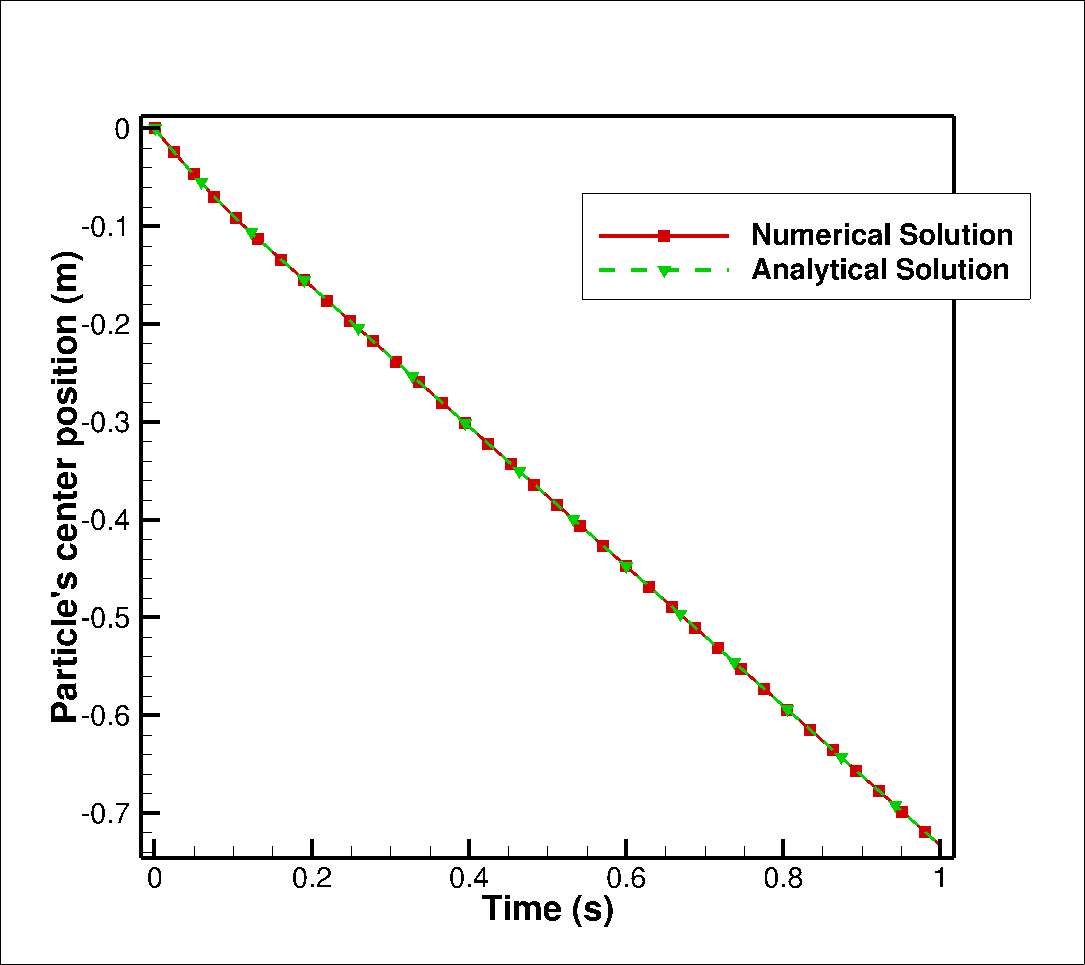
\includegraphics[width=0.32\textwidth]{chapitres/chapitre_3/figures/pos.png}}
\hspace{\fill}
   \subfloat[\label{vel_slide_roll_one} ]{%
      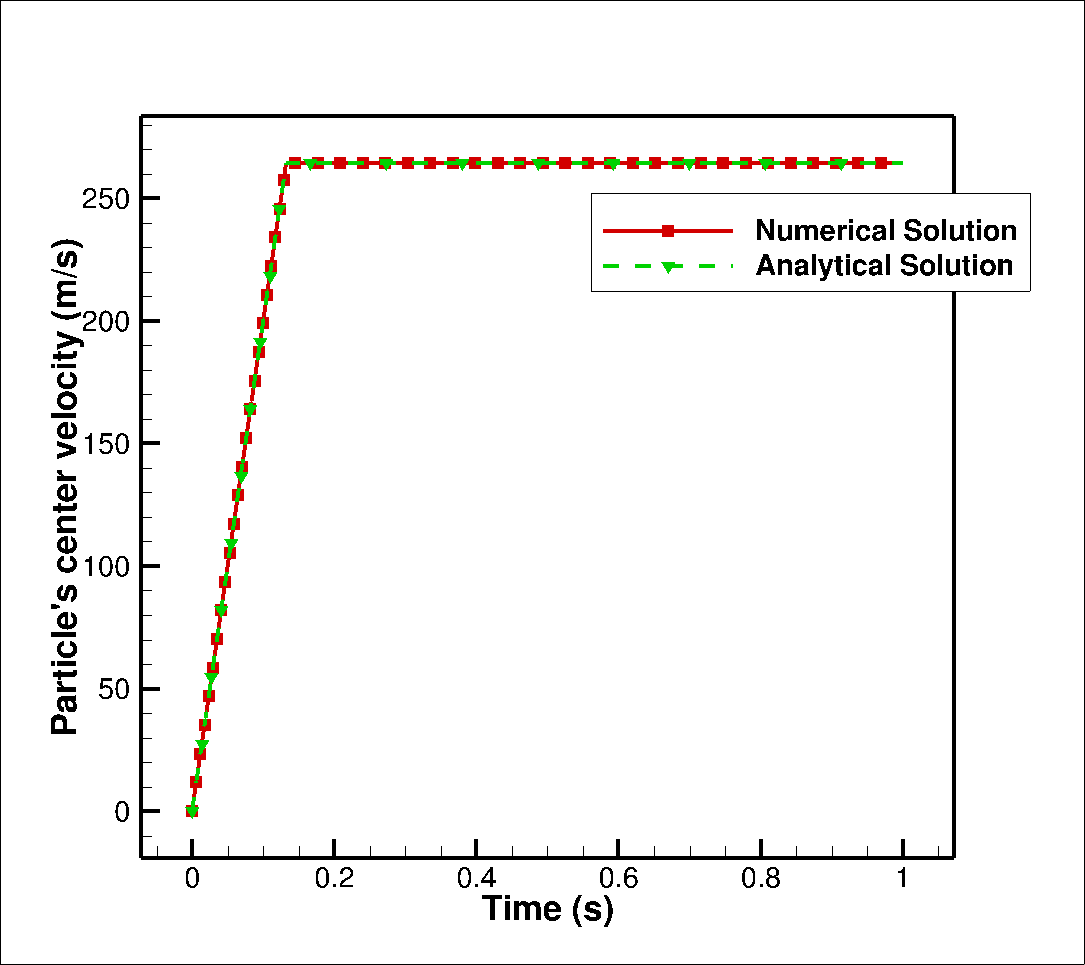
\includegraphics[width=0.32\textwidth]{chapitres/chapitre_3/figures/vel.png}}
\hspace{\fill}
   \subfloat[\label{rad_slide_roll_one}]{%_{nlgs}
      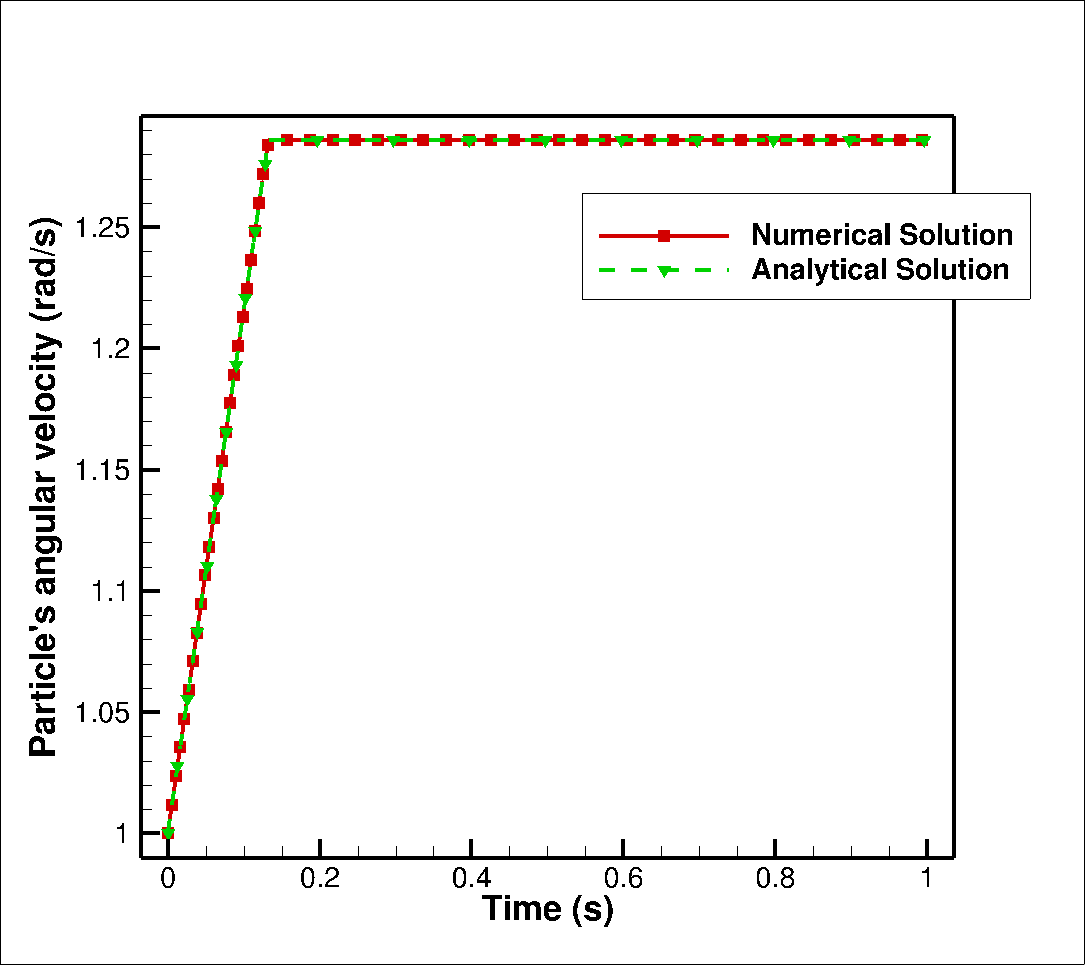
\includegraphics[width=0.32\textwidth]{chapitres/chapitre_3/figures/rad.png}}\\
\caption{\label{slide_roll_one}Comparaison entre la solution numérique et la solution analytique pour la bille d'acier en roulement glissement. (a) position; (b) Vitesse de roulement; (c) Vitesse angulaire.}
\end{figure*}


Les graphes de la Figure \ref{slide_roll_one} montrent que les courbes donnant les solutions numériques et analytique sont identiques, aussi bien à l'étape de roulement qu'à celle du glissement. De plus, on peut remarquer (voir Table \ref{tab14}) que l'erreur absolue entre la solution numérique et la solution analytique de la position, vitesse de roulement et vitesse angulaire est nulle, ce qui nous permet de valider notre modèle dans ce cas de figure.

\begin{center}
\begin{table}[!h]
\begin{tabular}{ |p{2.2cm}|p{3cm}|p{3cm}|p{3.5cm}| }

 \hline \rowcolor{lightgray}
 Pas de temps& Erreur absolue position& Erreur absolue vitesse angulaire& Erreur absolue vitesse de roulement\\
 \hline
 $1.32\times10^{-7}$ & $7.83\times10^{-11}$& $1.97\times10^{-8}$& $5.32\times10^{-11}$ \\
 $6.62\times10^{-6}$ & $2.21\times10^{-11}$& $4.70\times10^{-9}$& $1.27\times10^{-11}$ \\
 $1.32\times10^{-6}$ & $1.59\times10^{-12}$& $1.44\times10^{-9}$& $3.88\times10^{-12}$ \\
 $2.65\times10^{-6}$ & $1.73\times10^{-12}$& $1.41\times10^{-9}$& $3.52\times10^{-12}$ \\
 $1.32\times10^{-5}$ & $5.18\times10^{-13}$& $2.03\times10^{-10}$& $3.83\times10^{-13}$ \\
 \hline
\end{tabular}
\caption{
Erreur absolue entre la solution numérique et la solution analytique sur la position, la vitesse angulaire et la vitesse de roulement pour différents pas de temps.}\label{tab14}
\end{table}
\end{center}

En ce qui concerne les temps de calcul (voir Table \ref{tab15}), Les méthodes PDAS, SAL et IBP nécessitent un temps CPU total similaire pour le calcul de la solution. D'autre part, les méthodes PDAS nécessitent $2$ itérations NLGS pour converger à l'étape de glissement, $ 3 $ à l'étape de roulement, ce qui signifie que le bon état du contact avec frottement est directement trouvé. Pour la méthode SAL, $20$ itérations NLGS sont nécessaires pour converger. La méthode IBP quant à elle converge en $2$ itérations NLGS. 

\begin{center}
\begin{table}[!h]
\begin{tabular}{ |p{3cm}|p{3cm}|p{3cm}|p{2.6cm}| }

 \hline \rowcolor{lightgray}
 Méthode numérique& NLGS it. (Étape de glissement)& NLGS it. (Étape de roulement)& Temps CPU (s)\\
 \hline
 $EPDAS$ & $2$& $3$& $0.664$\\
 $IPDAS$ & $2$& $3$& $0.692$\\
 $SAL$ & $20$& $20$& $1.584$\\
 $IBP$ & $2$& $2$& $0.744$\\
 \hline
\end{tabular}
\caption{Nombre d'itérations NLGS nécessaire à chaque méthode (deuxième colonne) et temps CPU total (troisième colonne).}\label{tab15}
\end{table}
\end{center}
%------------------------------------------------------------------


%------------------------------------------------------------------

\subsection{Roulement glissement d'une bille d'acier dans une tambour fixe}\label{ex2}

Nous allons considérer dans cette partie un autre exemple représentatif, la même bille d'acier que la précédente, posée à l'intérieur d'un tambour fixe (voir Figure \ref{1_ball_drum}), avec une vitesse de translation horizontale initiale non nulle ($ v_0 = 0.5 m.s ^ { -1} $). Nous fournissons ci-dessous une description des paramètres physiques:


\begin{figure}[h!]
	\begin{center}
		\resizebox{6cm}{!}{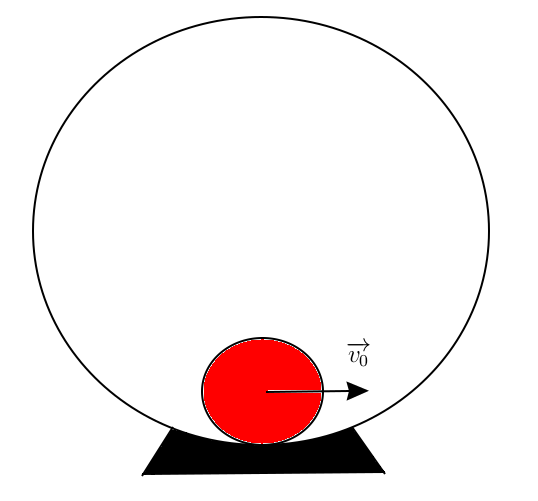
\includegraphics{chapitres/chapitre_3/figures/tambour_1_bille.png}}
	\end{center}
	\caption{Roulement glissement d'une bille d'acier dans un tambour fixe.}
	\label{1_ball_drum}
\end{figure}

\begin{eqnarray*}
	\begin{array}{l}
	    \rho=8000\ Kg/m^3, \quad r = 2.7\times10^{-3}\ m,\nonumber\\[2mm]
		Rayon\ tambour\ fixe: 0.05\ m,\nonumber\\[2mm]   
		g = -9.80665\ m/s^2 \nonumber\\[2mm]
	\end{array}
\end{eqnarray*}

Le comportement dynamique de la bille est similaire à celui d'un pendule. En effet, la bille atteint une position maximale, position pour laquelle la vitesse de translation de la bille est nulle. De plus, comme il y a du frottement avec la paroi du tambour, la bille a une vitesse angulaire qui varie au cours du temps. Les valeurs des paramètres numériques sont les suivantes:

\begin{eqnarray*}
	\begin{array}{l}
	    T = 5\ s,\quad dt = 2.5\times10^{-5}\ s, \nonumber \\[2mm]
		e_n = 1.0,\quad e_t = 1.0,\quad \mu = 0.22, \nonumber \\[2mm]
		\gamma_n = 10,\quad \gamma_t = 10, \quad r_{SAL} = r_{IBP} =  \frac{m}{dt} \nonumber  \\[2mm]
		\theta = 0.5,\quad {\rm crit\grave{e}re \quad d'arr\hat{e}t} \quad \epsilon_{NLGS} = 10^{-8}
	\end{array}
\end{eqnarray*}

\begin{figure*}[h!]
   \subfloat[\label{rad_slide_roll_drum}]{%
      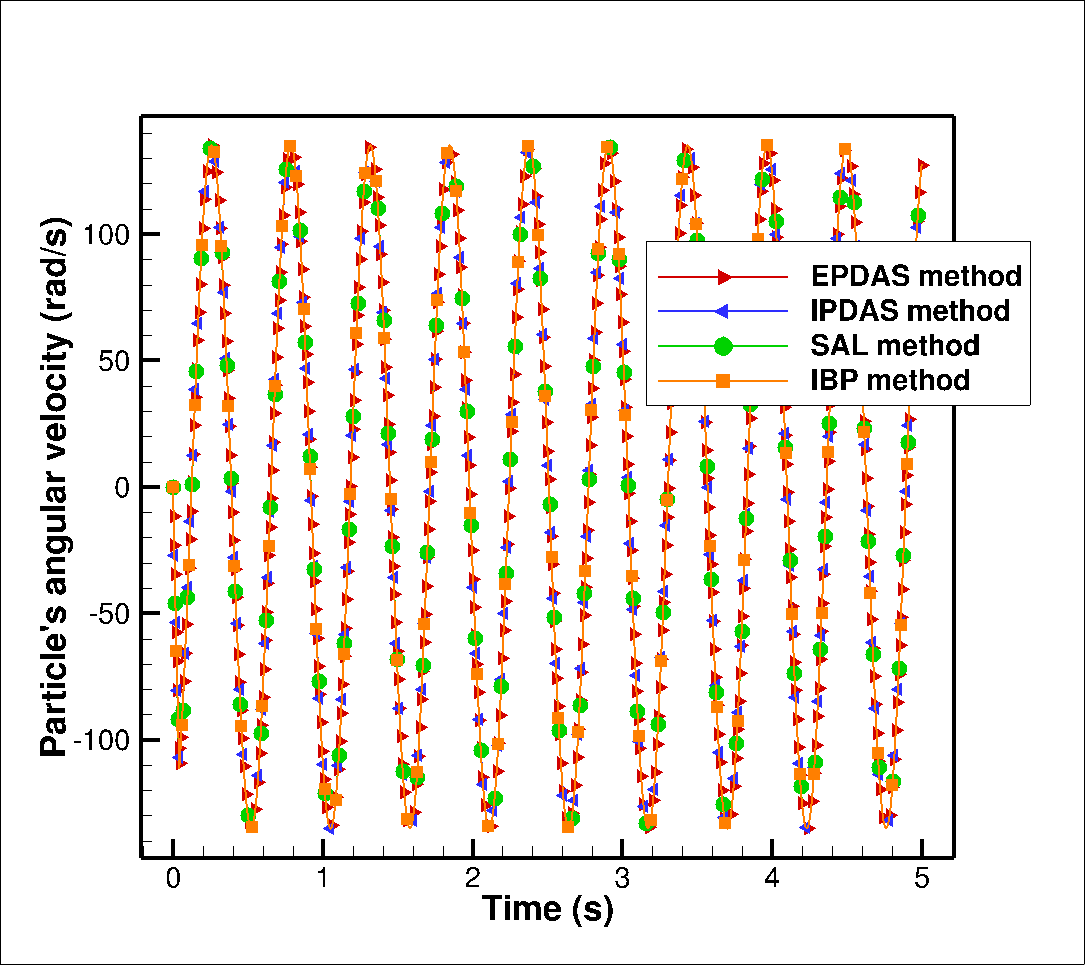
\includegraphics[trim=30 20 50 40,clip, width=0.5\textwidth]{chapitres/chapitre_3/figures/rad_PDAS_gamma=10.png}}
\hspace{\fill}
   \subfloat[\label{em_slide_roll_drum} ]{%
      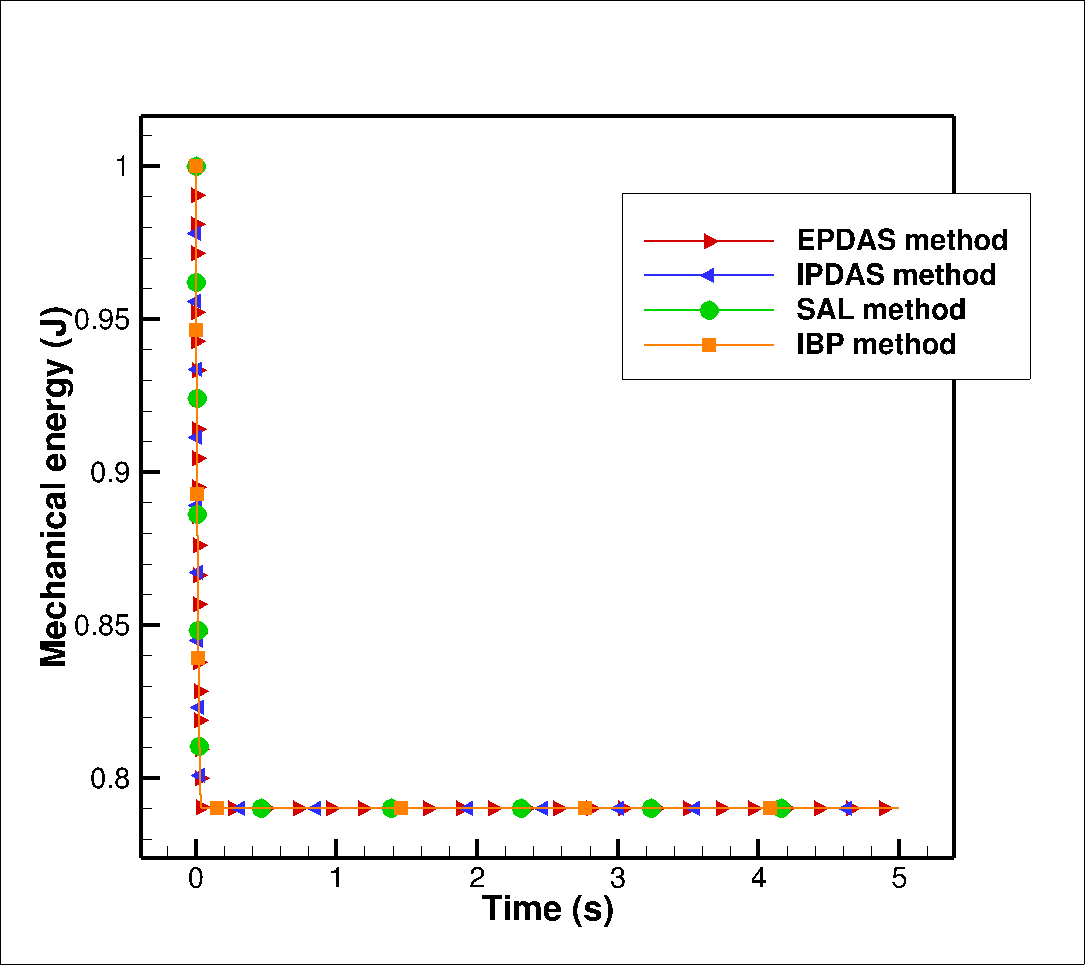
\includegraphics[trim=30 20 50 40,clip, width=0.5\textwidth]{chapitres/chapitre_3/figures/em_PDAS_gamma=10.png}}\\
\caption{\label{slide_roll_drum}Évolution au cours du temps de deux variables caractéristiques pour la bille d'acier dans un tambour fixe. (a) Dérivée temporelle de l'angle de repérage de la bille; (b) Énergie mécanique.}
\end{figure*}

La Figure \ref{rad_slide_roll_drum} décrit l'évolution de la dérivée temporelle de l'angle de repérage de la bille au cours du temps lors du processus de roulement glissement à l'intérieur du tambour fixe. Puisqu'il y a du frottement, la bille d'acier glisse jusqu'à ce que la dérivée temporelle de l'angle atteigne une valeur de $ -110\ rad / s $, puis commence à rouler. On observe que la dérivée temporelle de l'angle oscille au cours du temps et atteint son maximum en valeur absolue. Cette valeur maximale ne diminue pas lors de l'étape de roulement et atteint la même valeur maximale, car il n'y a plus de frottement et $e_n = 1$.\\
La Figure \ref{em_slide_roll_drum} montre l'évolution de l'énergie mécanique du système au cours du temps pendant le processus de roulement glissement à l'intérieur du tambour fixe. Elle diminue brutalement lors de l'étape de glissement à cause du frottement, puis elle est conservée lors de l'étape de roulement.

\begin{center}
\begin{table}[!h]
\begin{tabular}{ |p{4cm}|p{4cm}|p{4cm}| }

 \hline \rowcolor{lightgray}
 Méthode numérique& itérations NLGS& Temps CPU (s)\\
 \hline
 $EPDAS$ & $3$& $1.396$\\
 $IPDAS$ & $3$& $1.356$\\
 $SAL$ & entre $30$ et $40$& $5.224$\\
 $IBP$ & $2$& $1.844$\\
 \hline
\end{tabular}
\caption{Nombre d'itérations NLGS nécessaire à chaque méthode (deuxième colonne) et temps CPU total (troisième colonne).}\label{tab16}
\end{table}
\end{center}

Il est à noter que toutes les méthodes nécessitent un temps CPU total similaire pour calculer la solution, à l'exception de la méthode SAL qui est plus coûteuse en temps de calcul (voir la Table \ref{tab16}). De plus, les méthodes PDAS n'ont besoin que de $ 3 $ itérations  NLGS pour converger, $ 2 $ pour la méthode IBP, tandis que la méthode SAL met plus de 30 itérations NLGS pour converger.
%------------------------------------------------------------------

%------------------------------------------------------------------

\subsection{Sédimentation d'une collection de particules}\label{ex3}

Pour mettre en avant les performances des méthodes PDAS, nous introduisons dans ce paragraphe une configuration de sédimentation d'un ensemble de particules rigides dans une boîte, en portant une attention particulière à la comparaison entre les méthodes PDAS et les méthodes standards utilisées pour calculer les impulsions de contact locales. Chaque particule rigide de la collection a une vitesse aléatoire initiale. La Figure \ref{sedim} illustre le processus de sédimentation de $100 $, $200 $, $400 $, $800 $ et $1600 $ particules. Pour chaque configuration, deux rayons différents sont considérés pour les particules. Ces valeurs de rayons sont reportées dans la Table \ref{tab17}. Nous fournissons ci-dessous les paramètres physiques utilisés pour la simulation:

\begin{eqnarray*}
	\begin{array}{l}
	    \rho=2600\ Kg/m^3, \quad r = (voir\ Table\ \ref{tab17}) ,\nonumber\\[2mm]
		Dimensions\ domaine: [0,0.012] \times [0,0.022]\ m^2,\nonumber\\[2mm] 
		g = -9.80665\ m/s^2, \quad v_0 = al\acute{e}atoire \nonumber\\[2mm]
	\end{array}
\end{eqnarray*}

\begin{center}
\begin{table}[!h]
\begin{tabular}{ |p{4cm}|p{4cm}|p{4cm}| }

 \hline \rowcolor{lightgray}
 Nombres de particules& Petit rayon (m)& Grand rayon (m)\\
 \hline
 $100$ & $2.5\times10^{-4}$& $5.0\times10^{-4}$\\
 $200$ & $2.5\times10^{-4}$& $4.5\times10^{-4}$\\
 $400$ & $1.2\times10^{-4}$& $2.6\times10^{-4}$\\
 $800$ & $1.2\times10^{-4}$& $2.3\times10^{-4}$\\
 $1600$ & $6.0\times10^{-5}$& $1.3\times10^{-4}$\\
 \hline
\end{tabular}
\caption{Variation des rayons pour chaque configuration de sédimentation.}\label{tab17}
\end{table}
\end{center}


\begin{figure*}[h!]
   \subfloat[\label{sedim_100_1}]{%
      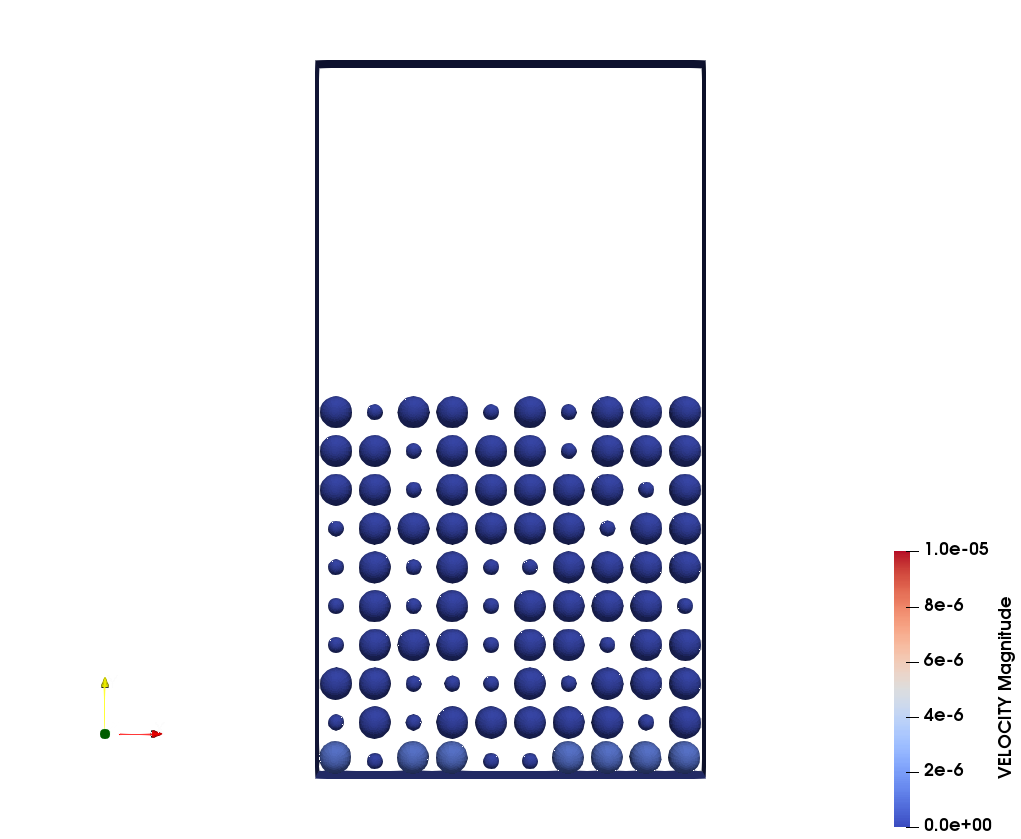
\includegraphics[trim=100 50 10 60,clip, width=0.32\textwidth]{chapitres/chapitre_3/figures/sedim_100_1.png}}
\hspace{\fill}
   \subfloat[\label{sedim_100_2} ]{%
      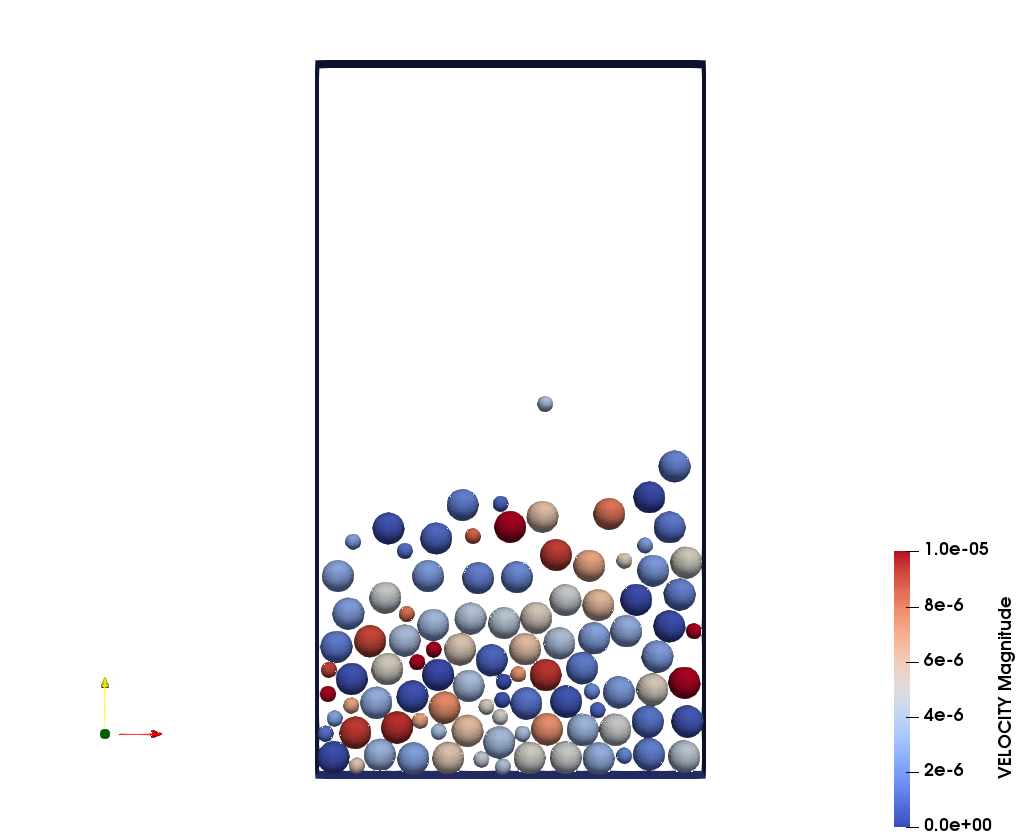
\includegraphics[trim=100 50 10 60,clip, width=0.32\textwidth]{chapitres/chapitre_3/figures/sedim_100_2.png}}
\hspace{\fill}
   \subfloat[\label{sedim_100_3}]{%
      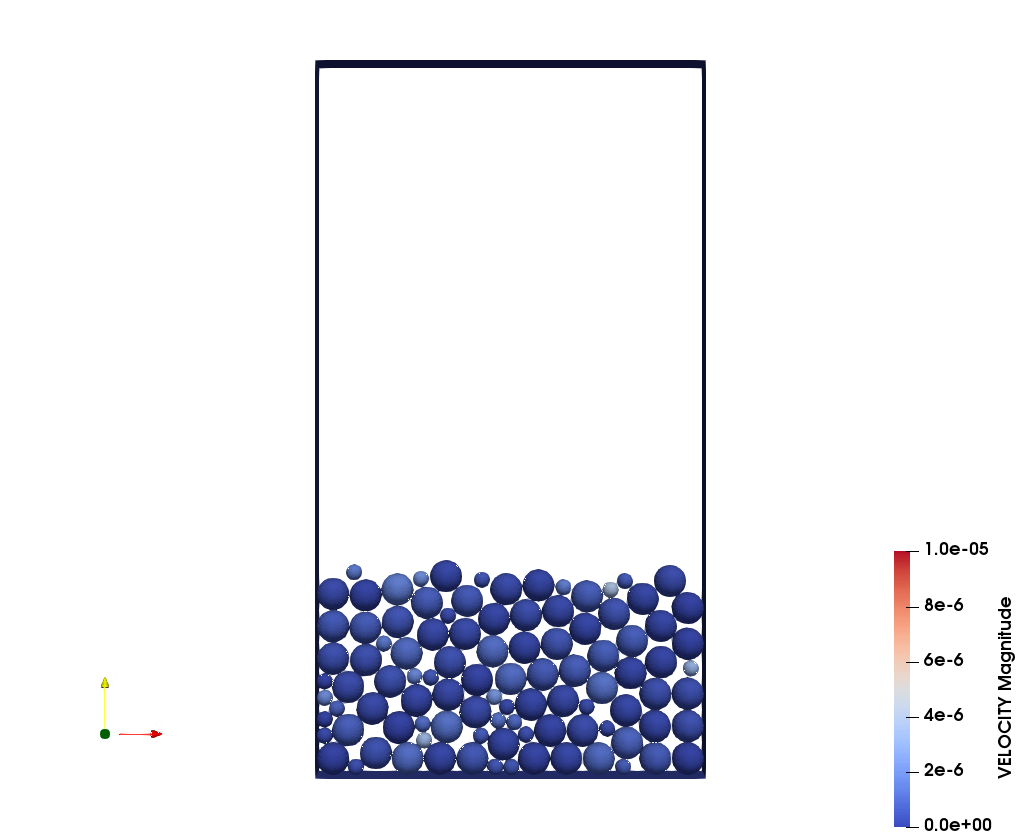
\includegraphics[trim=100 50 10 60,clip, width=0.32\textwidth]{chapitres/chapitre_3/figures/sedim_100_3.png}}\\
\hspace{\fill}
   \subfloat[\label{sedim_400_1}]{%
      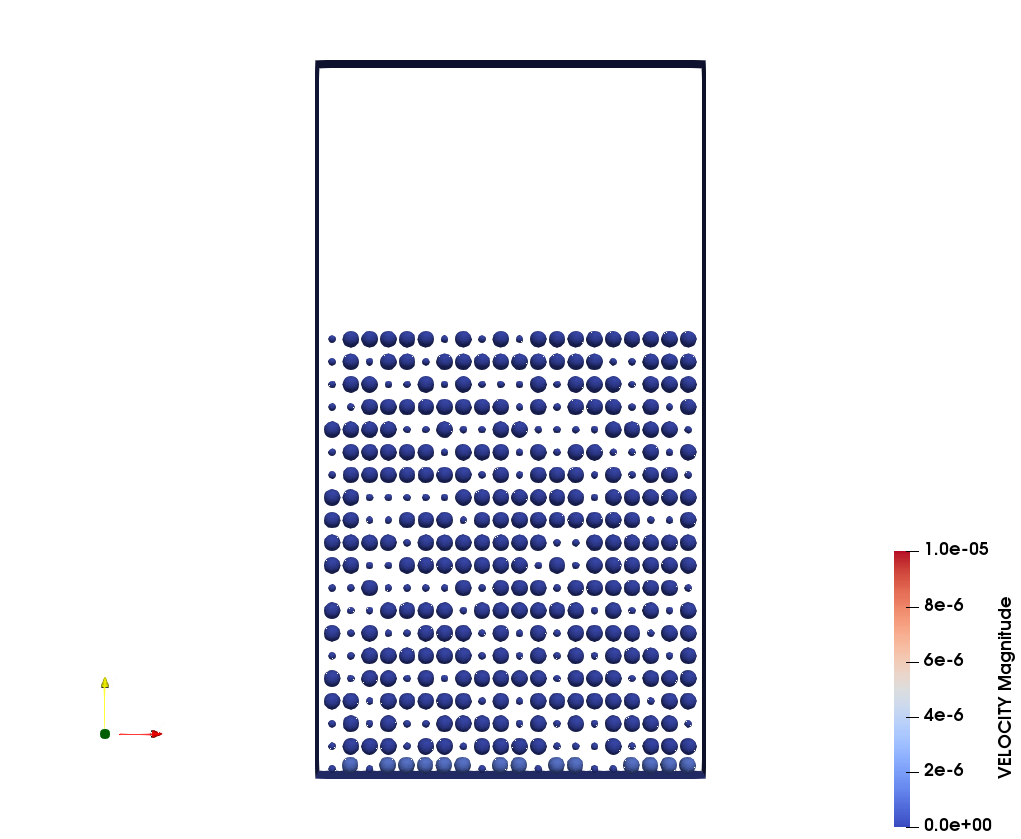
\includegraphics[trim=100 50 10 60,clip, width=0.32\textwidth]{chapitres/chapitre_3/figures/sedim_400_1.png}}
\hspace{\fill}
   \subfloat[\label{sedim_400_2} ]{%
      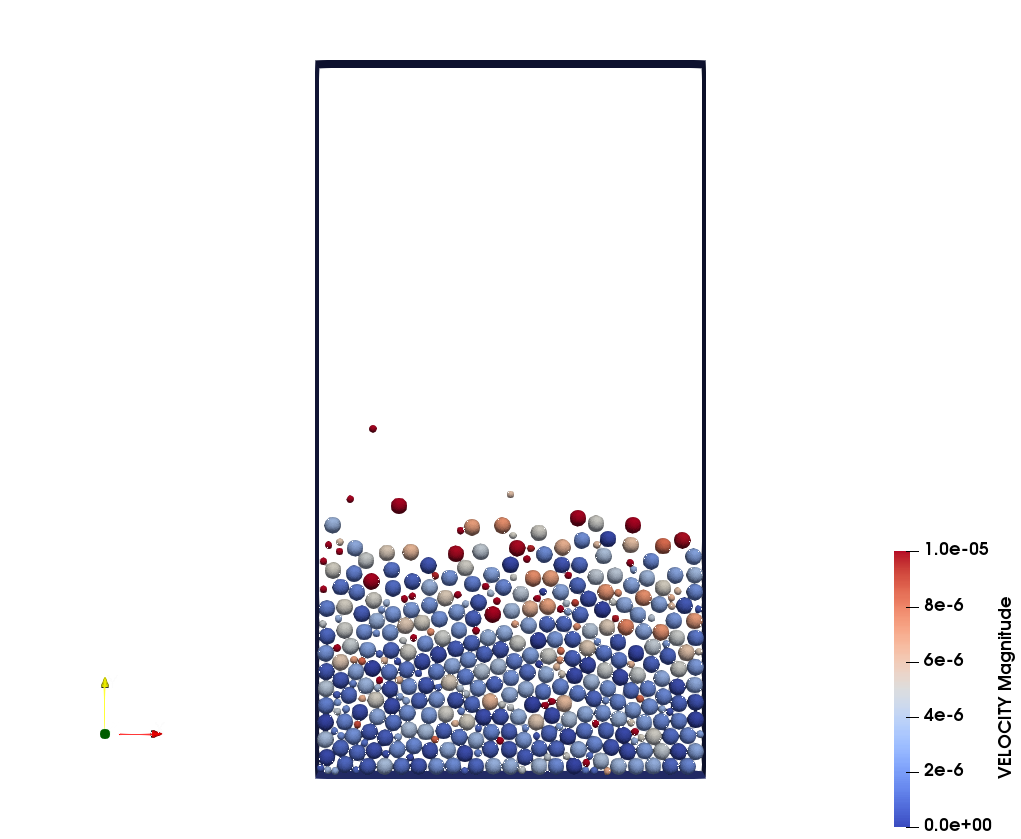
\includegraphics[trim=100 50 10 60,clip, width=0.32\textwidth]{chapitres/chapitre_3/figures/sedim_400_2.png}}
\hspace{\fill}
   \subfloat[\label{sedim_400_3}]{%
      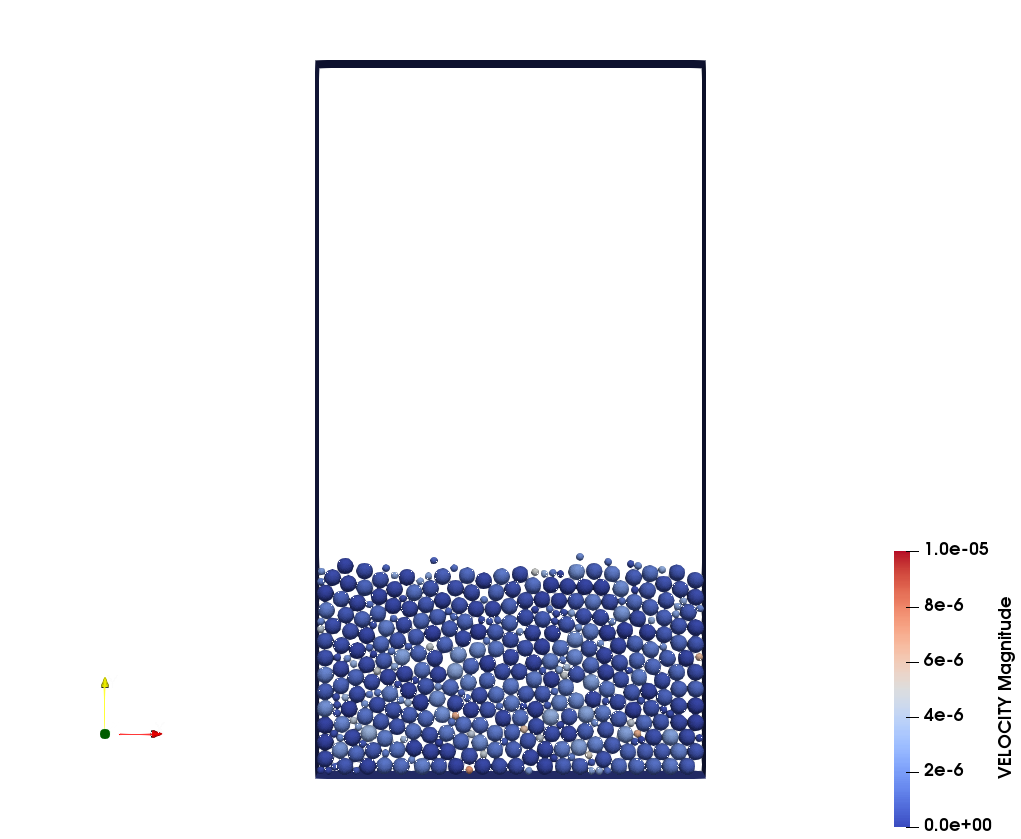
\includegraphics[trim=100 50 10 60,clip, width=0.32\textwidth]{chapitres/chapitre_3/figures/sedim_400_3.png}}\\
\hspace{\fill}
   \subfloat[\label{sedim_1600_1}]{%
      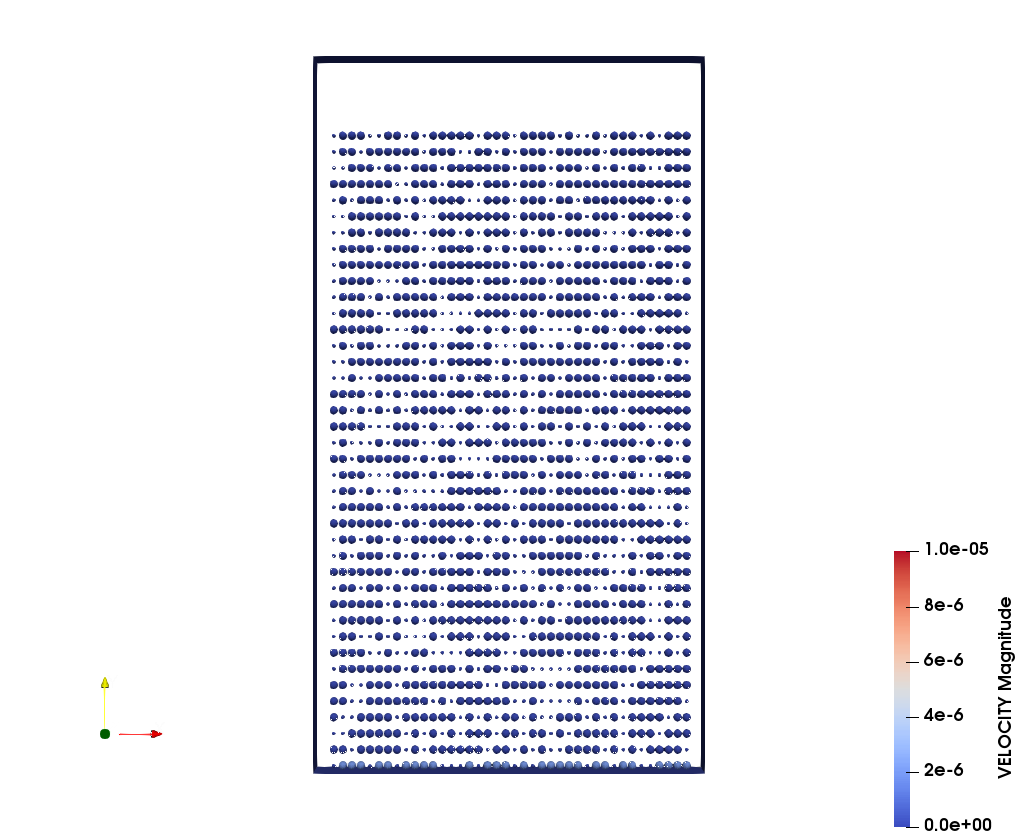
\includegraphics[trim=100 50 10 60,clip, width=0.32\textwidth]{chapitres/chapitre_3/figures/sedim_1600_1.png}}
\hspace{\fill}
   \subfloat[\label{sedim_1600_2} ]{%
      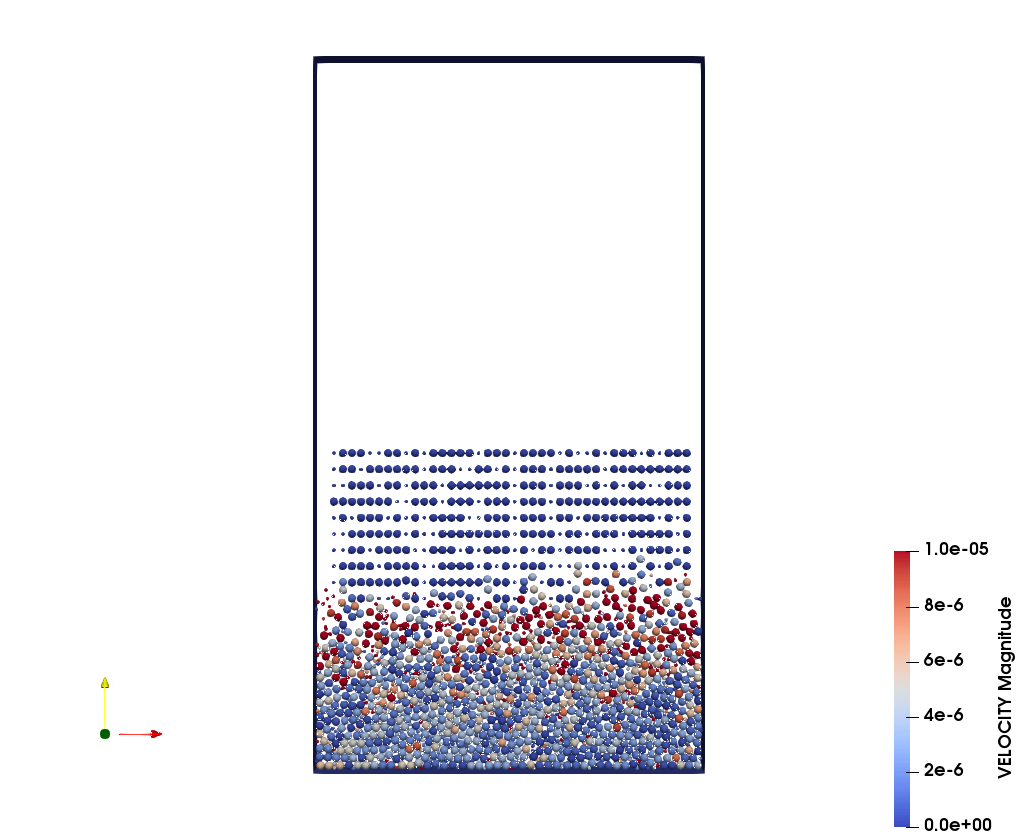
\includegraphics[trim=100 50 10 60,clip, width=0.32\textwidth]{chapitres/chapitre_3/figures/sedim_1600_2.png}}
\hspace{\fill}
   \subfloat[\label{sedim_1600_3}]{%
      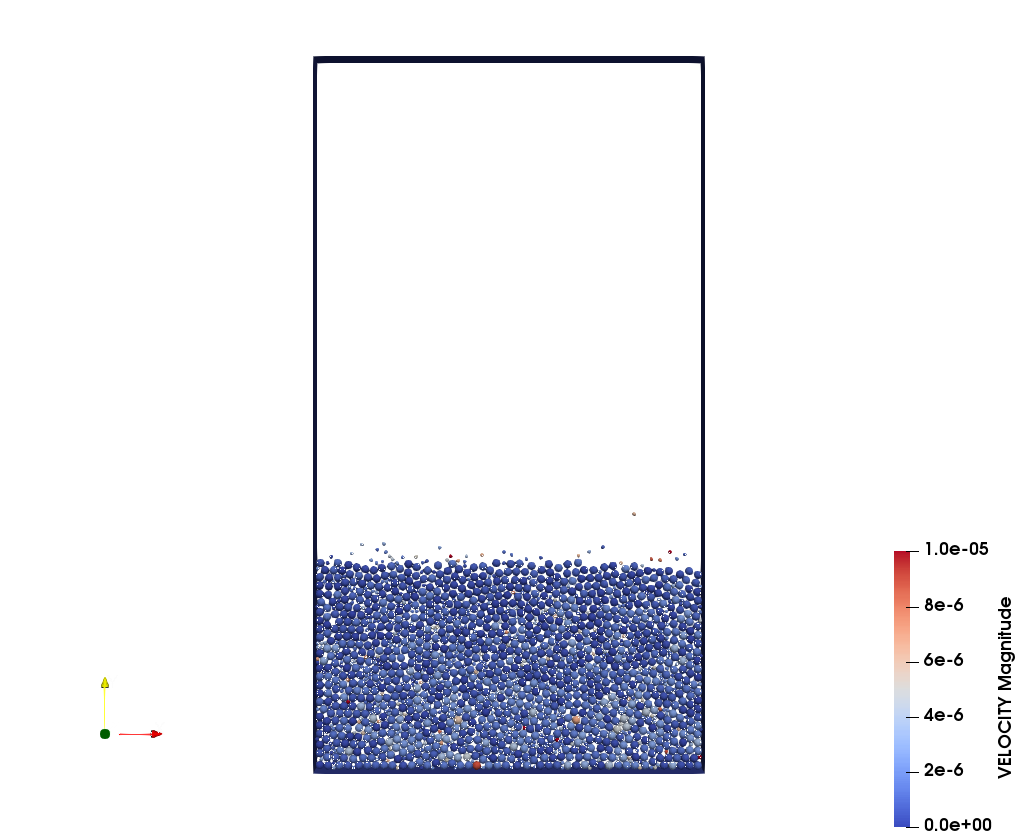
\includegraphics[trim=100 50 10 60,clip, width=0.32\textwidth]{chapitres/chapitre_3/figures/sedim_1600_3.png}}\\
\caption{\label{sedim}Processus de sédimentation d'une collection de particules rigides dans une boîte au cours du temps. [(a), (b), (c)]$ 100 $ particules, [(d), (e), (f)]$ 400 $ particules, [(g), (h), (i)]$ 1600 $ particules.}
\end{figure*}

\noindent La simulation est réalisée sur $ 1 $ seconde, les paramètres numériques relatifs à cette simulation sont les suivants:

\begin{eqnarray*}
	\begin{array}{l}
	    T = 1\ s,\quad dt = 10^{-4}\ s, \nonumber \\[2mm]
		e_n = 1.0,\quad e_t = 1.0,\quad \mu = 0.2, \nonumber \\[2mm]
		\gamma_n = 10^{-4},\quad \gamma_t = 10^{-9}, \quad r_{SAL} = r_{IBP} = \frac{m}{dt} \nonumber  \\[2mm]
		\theta = 0.5,\quad {\rm crit\grave{e}re \quad d'arr\hat{e}t} \quad \epsilon_{NLGS} = 10^{-6}
	\end{array}
\end{eqnarray*}

Cet exemple est représentatif des simulations en milieu granulaire en raison du grand nombre de corps rigides impliqués, des nombreux contacts simultanés et des temps de calcul importants. D'après les graphes de la Figure \ref{cumul_cpu}, nous observons que les méthodes EPDAS et IPDAS fournissent les meilleurs résultats en termes de temps de calcul pendant tout le processus de sédimentation pour $ 100 $, $200 $, $400 $, $800 $ et $1600 $ particules. En effet, le temps cumulé nécessaire pour calculer les impulsions de contact à l'aide de la méthode PDAS augmente faiblement au cours du temps comparé aux méthodes SAL et IBP, qui nécessitent un temps CPU plus important pour calculer la solution. Pour un grand nombre de particules impliquées, la Table \ref{tab18} reprend les valeurs des temps CPU totaux pour chaque méthode numérique.\\


\begin{figure*}[h!]
   \subfloat[\label{cumul_cpu_100}]{%
      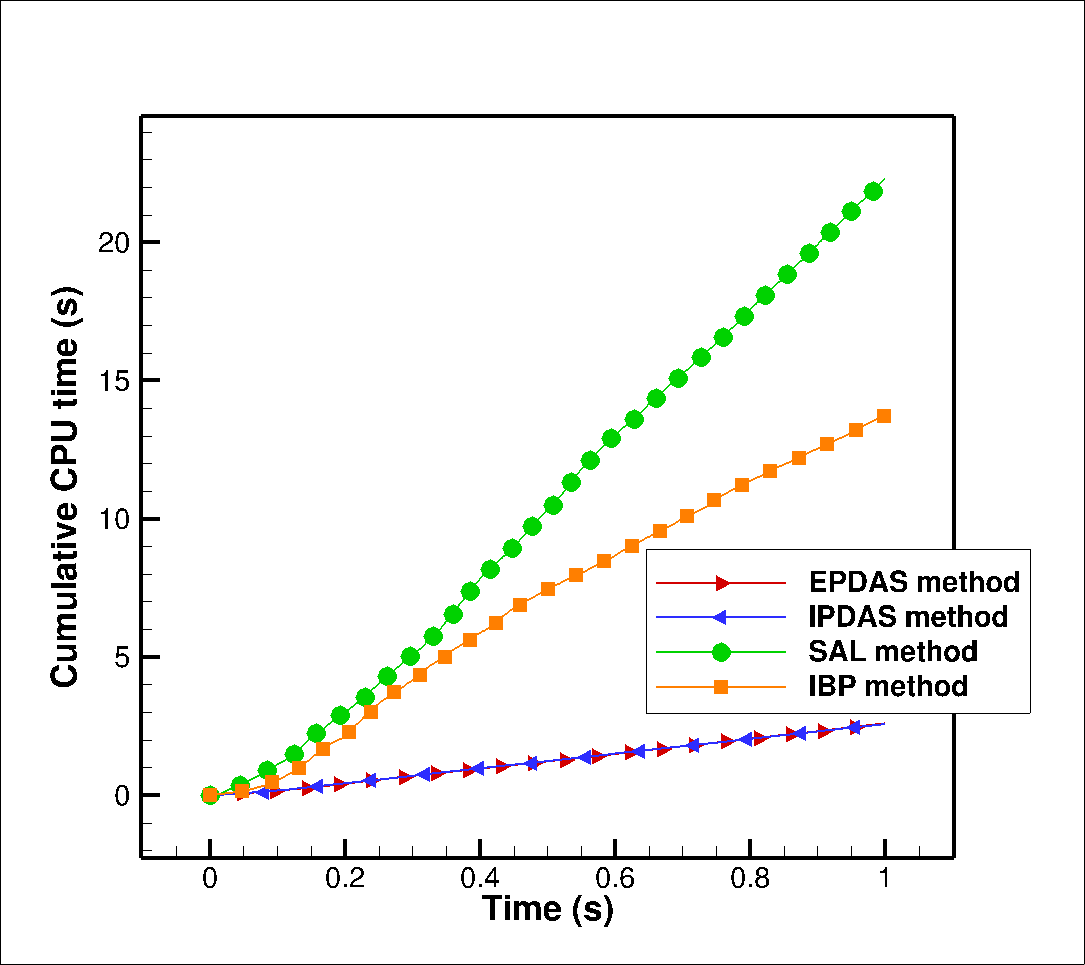
\includegraphics[trim=30 30 50 30,clip, width=0.5\textwidth]{chapitres/chapitre_3/figures/cumul_cpu_100.png}}
\hspace{\fill}
   \subfloat[\label{cumul_cpu_200} ]{%
      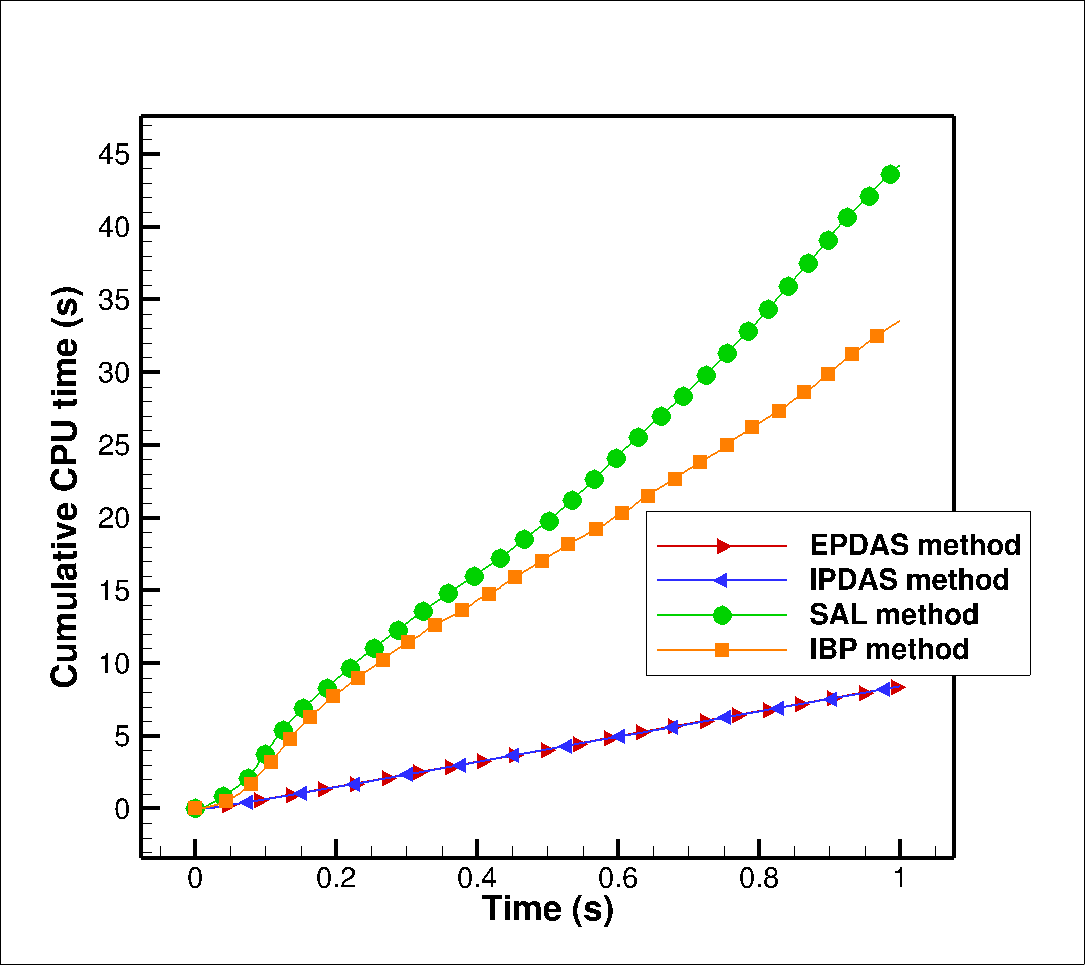
\includegraphics[trim=30 30 50 30,clip, width=0.5\textwidth]{chapitres/chapitre_3/figures/cumul_cpu_200.png}}\\
\caption{\label{cumul_cpu}Évolution du temps CPU cumulé nécessaire pour calculer les impulsions de contact pendant le processus de sédimentation. (a) $100 $ particules, (b) $200 $ particules.}
\end{figure*}

\begin{table}[!h]
\begin{tabular}{|p{2cm}|p{1.75cm}|p{1.75cm}|p{1.75cm}|p{1.9cm}|p{1.9cm}|}
  \hline \rowcolor{lightgray}
  \multicolumn{6}{|c|}{Temps CPU total (s)} \\
  \hline \rowcolor{lightgray}
  Méthode numérique & 100 particules & 200 particules& 400 particules & 800 particules & 1600 particules \\ 
  \hline  EPDAS & $2.59$ & $8.41$ & $28.34$ & $107.91$ & $12298.42$\\
  IPDAS & $2.56$ & $8.39$ & $28.35$ & $105.41$ & $11515.38$\\
  SAL & $22.29$ & $44.21$ & $87.29$ & $182.14^{(*)}$ & $18673.19^{(*)}$\\
  IBP & $13.75$ & $33.53$ & $65.86$ & $186.39^{(*)}$ & $16798.55^{(*)}$\\ 
 \hline
\end{tabular}
 \caption{Temps CPU total consacré au calcul des impulsions de contact pendant le processus de sédimentation pour chaque méthode numérique et un nombre différent de particules rigides (voir remarque ci-dessous pour (*).}\label{tab18}
\end{table}

Par ailleurs, ce cas-test permet non seulement d'évaluer les performances des méthodes PDAS, mais aussi leur robustesse. Les graphes de la Figure \ref{cumul_nlgs} montrent l'évolution des itérations NLGS cumulées nécessaires à la convergence du calcul des impulsions de contact pendant le processus de sédimentation, et on peut noter que les courbes EPDAS et IPDAS sont assez similaires et ont tendance à converger plus rapidement que celle de la méthode SAL, et fournissent des résultats comparables avec la méthode IBP, en particulier à la fin du processus de sédimentation. Pour un grand nombre de particules impliquées, la Table \ref{tab19} reprend les valeurs totales des itérations NLGS nécessaires pour calculer la solution pour chaque méthode numérique.\\

\begin{figure*}[h!]
   \subfloat[\label{cumul_nlgs_100}]{%
      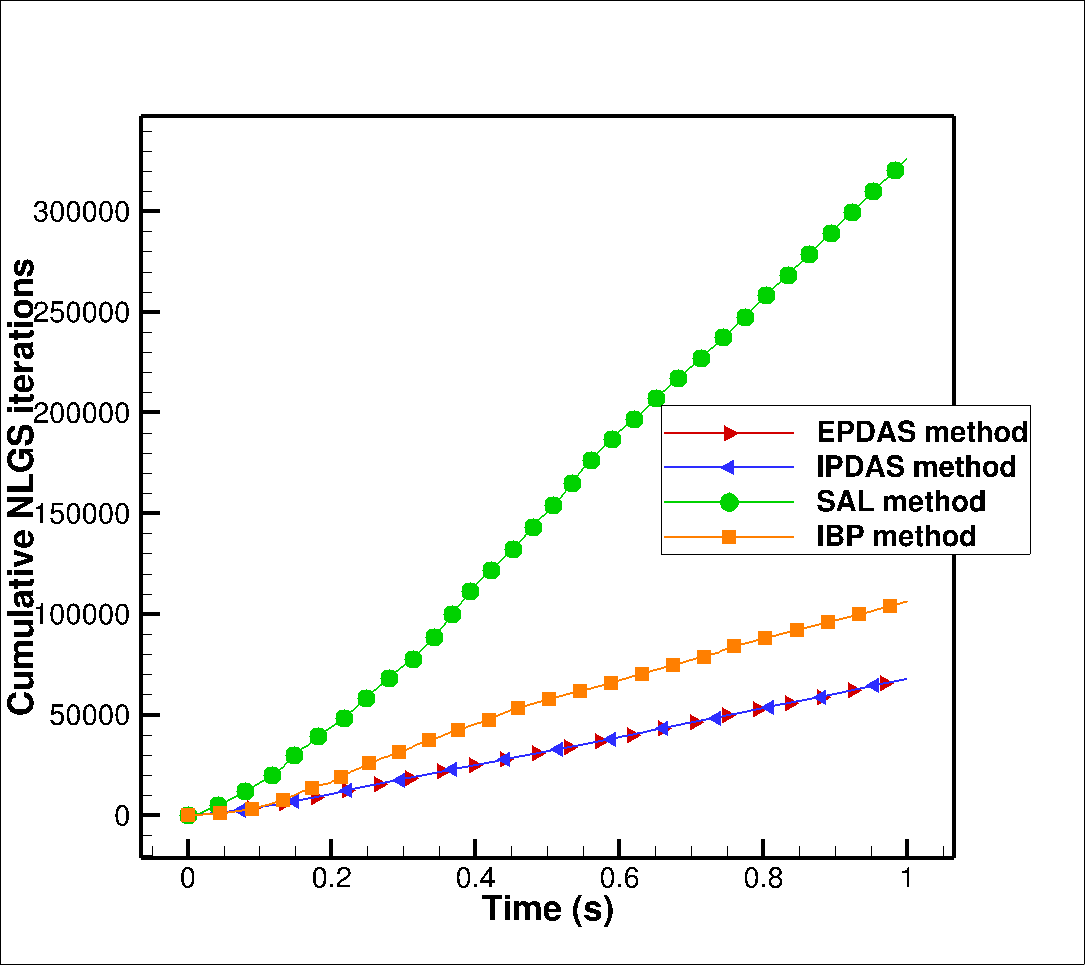
\includegraphics[trim=10 30 50 30,clip, width=0.5\textwidth]{chapitres/chapitre_3/figures/cumul_nlgs_100.png}}
\hspace{\fill}
   \subfloat[\label{cumul_nlgs_200} ]{%
      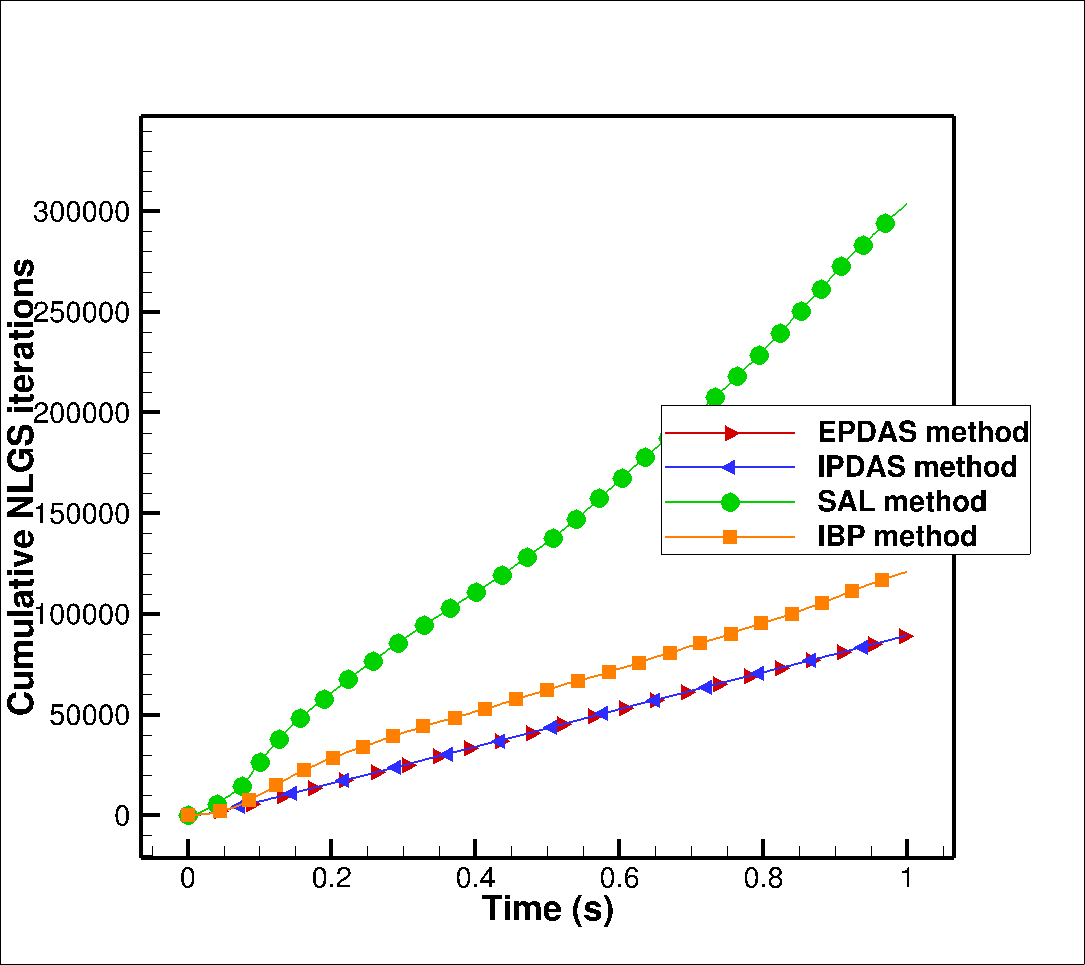
\includegraphics[trim=10 30 50 30,clip, width=0.5\textwidth]{chapitres/chapitre_3/figures/cumul_nlgs_200.png}}\\
\caption{\label{cumul_nlgs}Évolution du nombre cumulé d'itérations NLGS nécessaire à la convergence du calcul des impulsions de contact au cours du processus de sédimentation. (a) $100$ particules, (b) $200$ particules.}
\end{figure*}

\begin{table}[!h]
\begin{tabular}{|p{2cm}|p{1.75cm}|p{1.75cm}|p{1.75cm}|p{1.9cm}|p{1.9cm}|}
  \hline \rowcolor{lightgray}
  \multicolumn{6}{|c|}{Nombre total d'iterations NLGS} \\
  \hline \rowcolor{lightgray}
  Méthode numérique& 100 particules & 200 particules & 400 particules & 800 particules & 1600 particules \\ 
  \hline  EPDAS & $67726$ & $89347$ & $95995$ & $147445$ & $25578301$\\
  IPDAS & $67121$ & $85663$ & $99765$ & $142802$ & $23836195$\\
  SAL & $326121$ & $363596$ & $442943$ & $144305^{(*)}$ & $2648147^{(*)}$\\
  IBP & $106194$ & $120975$ & $138970$ & $83404^{(*)}$ & $1978658^{(*)}$\\ 
 \hline
\end{tabular}
 \caption{Nombre total d'itérations NLGS nécessaires au calcul des impulsions de contact pendant le processus de sédimentation pour chaque méthode numérique et un nombre différent particules rigides (voir remarque ci-dessous pour (*).}\label{tab19}
\end{table}

\noindent \begin{remarque1}
\textit{Les résultats marqués d'un astérisque dans les Tables \ref{tab18} et \ref{tab19} correspondent à des simulations réalisées avec les méthodes SAL et IBP où nous avons remarqué de grandes interpénétrations entre particules rigides à la fin du processus de sédimentation.}
\end{remarque1}

%------------------------------------------------------------------


%------------------------------------------------------------------

\subsection{Écoulement granulaire dans un tambour rotatif en 2D}\label{ex4}

Pour finir, nous considérons un dernier cas-test numérique de tambour rotatif dans lequel nous étudions l'écoulement d'un échantillon de billes d'acier. Les paramètres physiques et numériques de la simulation suivante ont été choisis de façon à correspondre à celle réalisée dans \cite{maione2015investigation} et ce, afin de fournir une comparaison entre l'expérience réalisée et les résultats numériques. La Figure \ref{rise_repose_drum_experim} présente à gauche une capture de l'expérience réalisée avec $1,5 $ Kg de billes d'acier dans un tambour rotatif à $40 $ rpm et la simulation DEM associée. Les billes d'acier ont tendance à s'organiser en couches: une couche en contact avec la paroi du tambour et le reste des billes sous formes de lit. Dans cette étude, les méthodes PDAS sont utilisées pour évaluer la hauteur moyenne de montée et l'angle moyen de repos lorsque la simulation atteint un état stable. Au-delà de la comparaison numérique, l'intérêt de cet exemple réside dans le fait qu'une telle expérience permet d'évaluer l'efficacité et la fiabilité des méthodes PDAS. \\

Ainsi, 5 simulations ont été réalisées avec différents échantillons de billes d'acier de même tailles ($ 100 $, $200 $, $400 $, $800 $ puis $1600 $) dans le tambour rotatif. Tout d'abord, nous fournissons ci-dessous une description des paramètres physiques communs aux simulations:

\begin{eqnarray*}
	\begin{array}{l}
	    Échantillons \ de\ particules: 100\ /\ 200\ /\ 400\ /\ 800\ /\ 1600,\nonumber\\[2mm]
	    Vitesse\ de\ rotation = 40\ rpm,\nonumber\\[2mm]
	    \rho=8000\ Kg/m^3, \quad r_p \leq 2.7\times10^{-3}\ m,\nonumber\\[2mm]
		Rayon\ du\ tambour: 0.05\ m,\nonumber\\[2mm] 
		g = -9.80665\ m/s^2,\nonumber\\[2mm]
	\end{array}
\end{eqnarray*}

\begin{figure}[h!]
	\begin{center}
		\resizebox{6cm}{!}{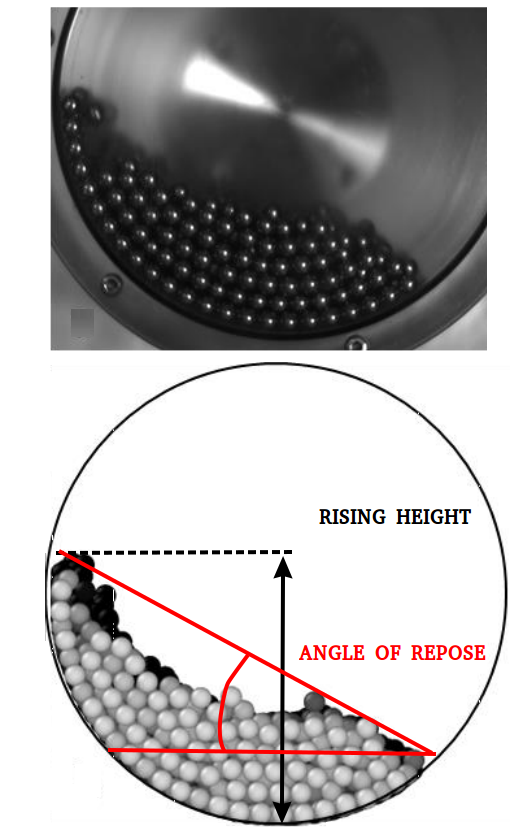
\includegraphics{chapitres/chapitre_3/figures/experim_these.png}}
	\end{center}
	\caption{Comparaison entre l'expérience et la simulation DEM réalisée dans \cite{maione2015investigation} avec des billes d'acier à l'intérieur d'un tambour rotatif.}
	\label{rise_repose_drum_experim}
\end{figure}

Les paramètres numériques communs aux simulations du tambour rotatif sont comme suit:

\begin{eqnarray*}
	\begin{array}{l}
	    T = 1\ s,\quad dt = 10^{-4}\ s, \nonumber \\[2mm]
		e_n = 0.6,\quad e_t = 1.0,\quad \mu = 0.22, \nonumber \\[2mm]
		\gamma_n = 10^{-8},\quad \gamma_t = 10^{-8}, \quad r_{SAL} = r_{IBP} = \frac{m}{dt} \nonumber  \\[2mm]
		\theta = 0.5,\quad {\rm crit\grave{e}re \quad d'arr\hat{e}t} \quad \epsilon_{NLGS} = 10^{-5}
	\end{array}
\end{eqnarray*}

Ces simulations sont représentatives des problèmes de contact multi-corps rigides du fait du grand nombre de contacts simultanés et du temps de CPU nécessaire pour calculer la solution. Lorsqu'un écoulement de surface régulier est atteint (voir Figure \ref{drum_PDAS}), nous constatons que l'angle moyen de repos et la hauteur moyenne de montée obtenus par les méthodes PDAS sont assez similaires à ceux observés sur la Figure \ref{rise_repose_drum_experim}, et ce quel que soit l'échantillon de billes. D'après \cite{maione2015investigation}, l'angle de repos résultant est égal à 26 $^{\circ}$. \\

\begin{figure*}[h!]
   \subfloat[\label{drum_100}]{%
      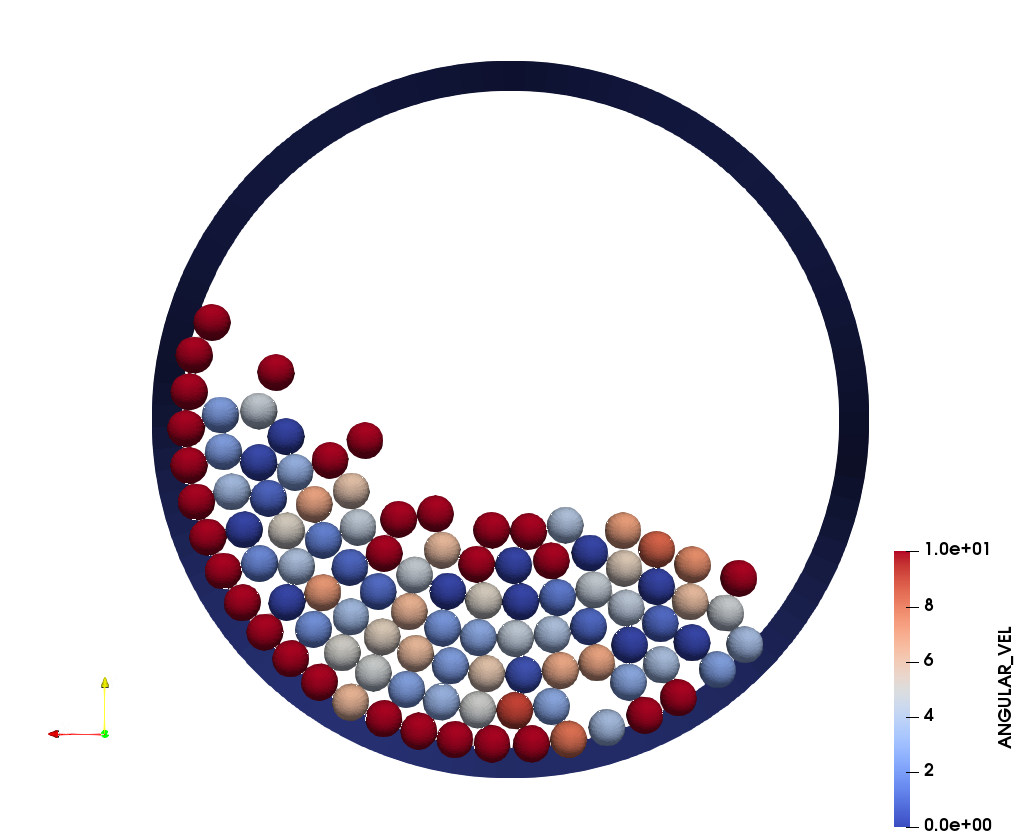
\includegraphics[trim=150 5 10 50,clip, width=0.32\textwidth]{chapitres/chapitre_3/figures/tambour_100.png}}
\hspace{\fill}
   \subfloat[\label{drum_400} ]{%
      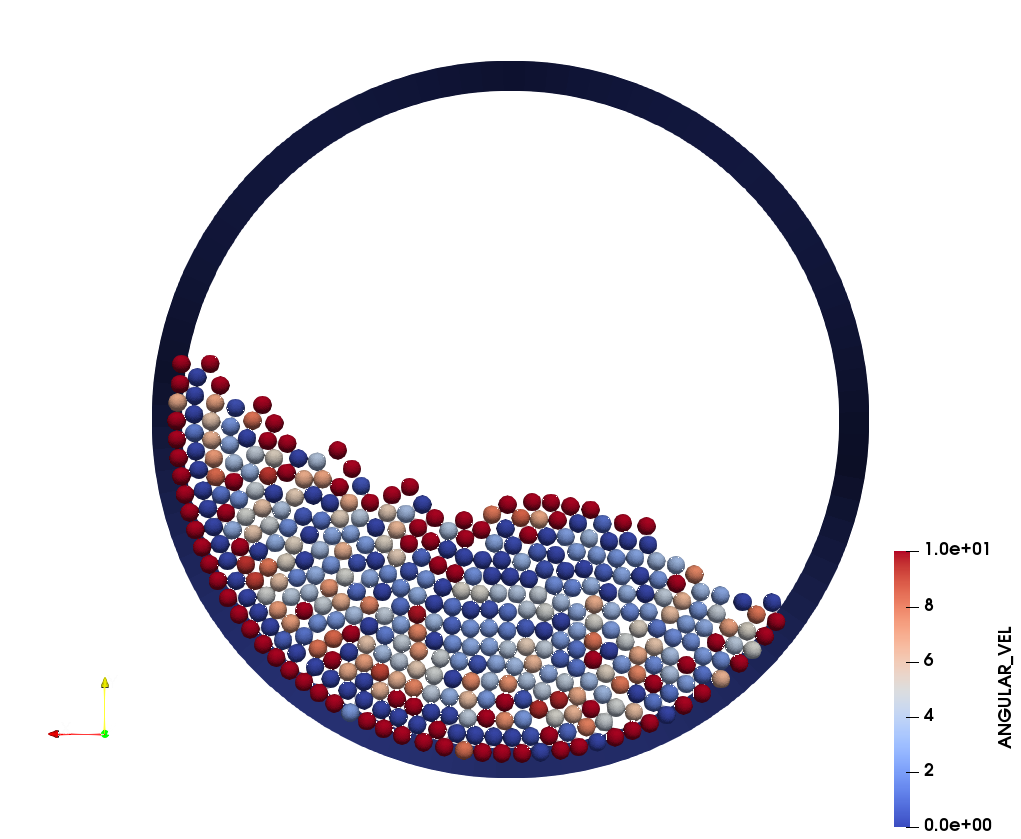
\includegraphics[trim=150 5 10 30,clip, width=0.32\textwidth]{chapitres/chapitre_3/figures/tambour_400.png}}
\hspace{\fill}
   \subfloat[\label{drum_1600}]{%
      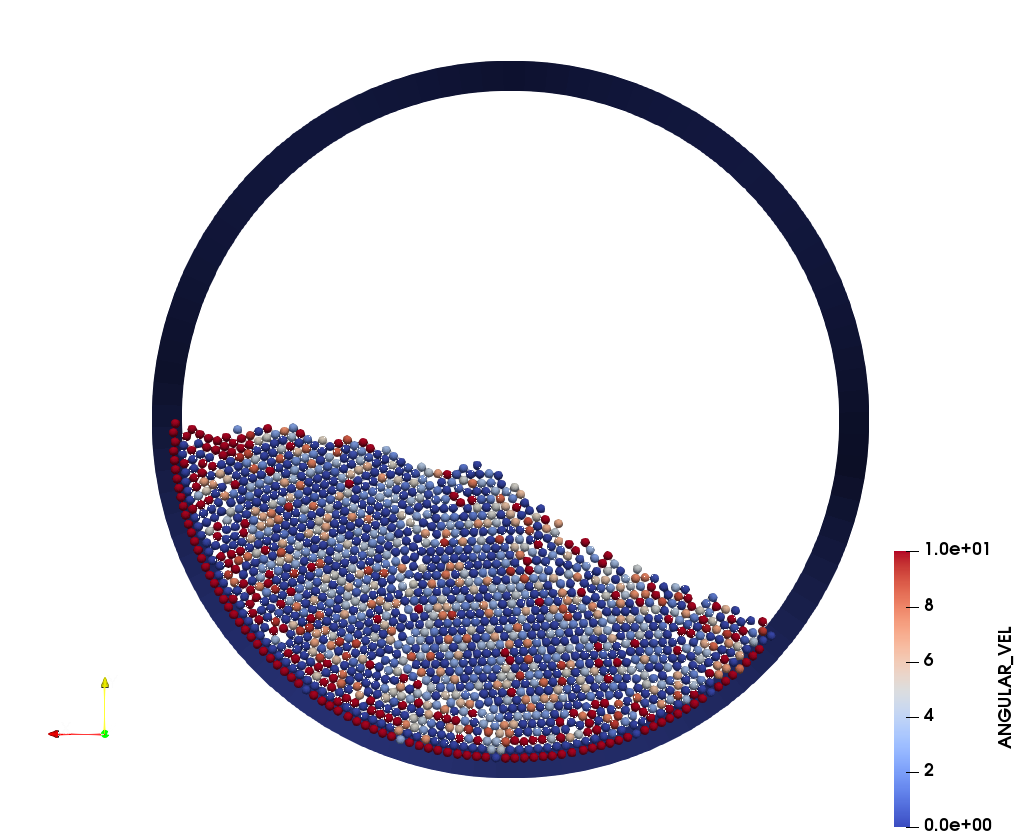
\includegraphics[trim=150 5 10 50,clip, width=0.32\textwidth]{chapitres/chapitre_3/figures/tambour_1600.png}}\\
\caption{\label{drum}Vues de perspective des simulations du tambour rotatif réalisées avec les méthodes PDAS (a) 100 billes d'acier, (b) 400 billes d'acier, 1600 billes d'acier lorsqu'un écoulement de surface régulier est atteint.}\label{drum_PDAS}
\end{figure*}

En ce qui concerne la convergence des méthodes numériques, les graphes de la Figure \ref{cumul_nlgs_tambour} permettent d'évaluer une fois de plus l'efficacité des méthodes PDAS, qui fournissent des résultats très comparables avec la méthode IBP. Les courbes EPDAS et IPDAS sont assez similaires et montrent que ces méthodes ont tendance à converger plus rapidement que la méthode SAL. Pour un échantillon de $1600$ billes d'acier par exemple (voir Table \ref{tab20}), le nombre d'itérations NLGS nécessaires pour calculer la solution varie de 8 à 10 millions pour les méthodes PDAS et IBP, alors que la méthode SAL nécessite plus de 30 millions d'itérations NLGS pour converger.\\


\begin{figure*}[h!]
   \subfloat[\label{cumul_nlgs_tambour_100}]{%
      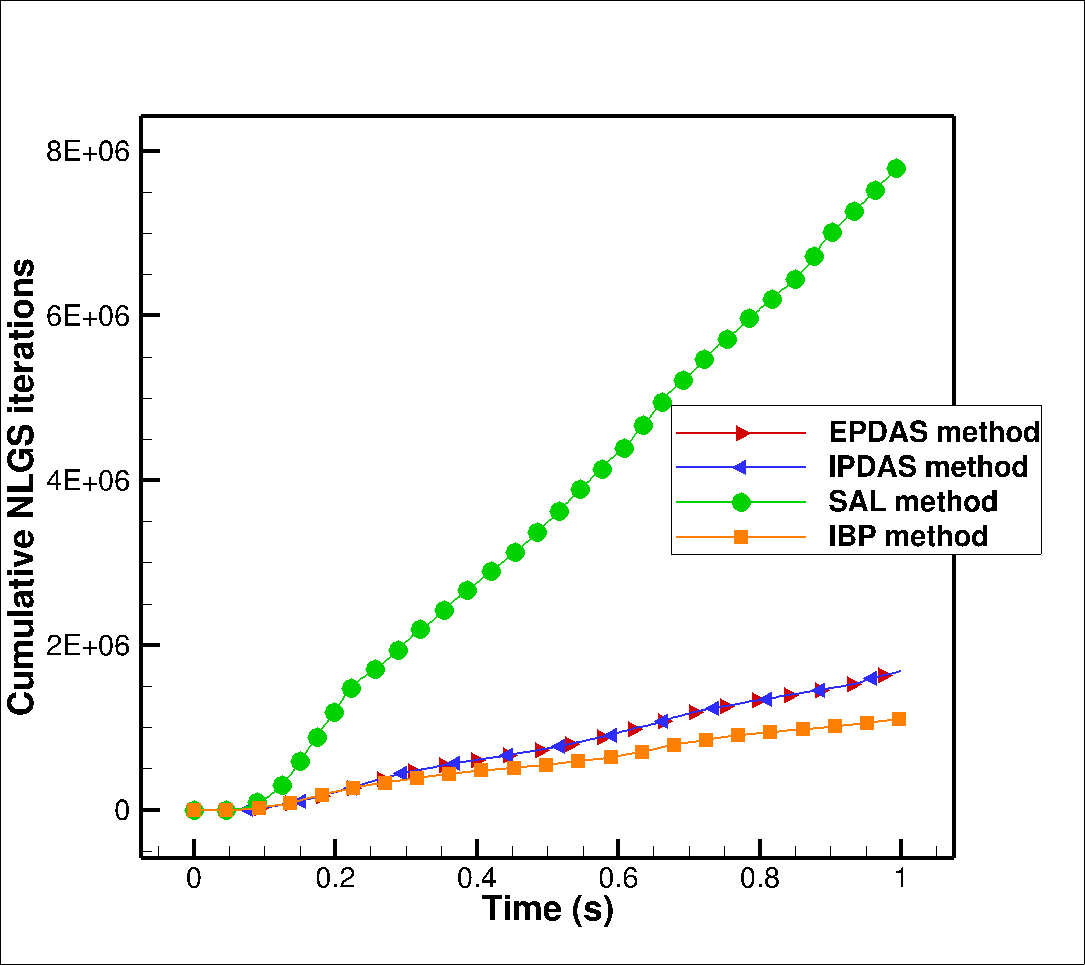
\includegraphics[width=0.32\textwidth]{chapitres/chapitre_3/figures/cumul_nlgs_tambour_100.png}}
\hspace{\fill}
   \subfloat[\label{cumul_nlgs_tambour_400} ]{%
      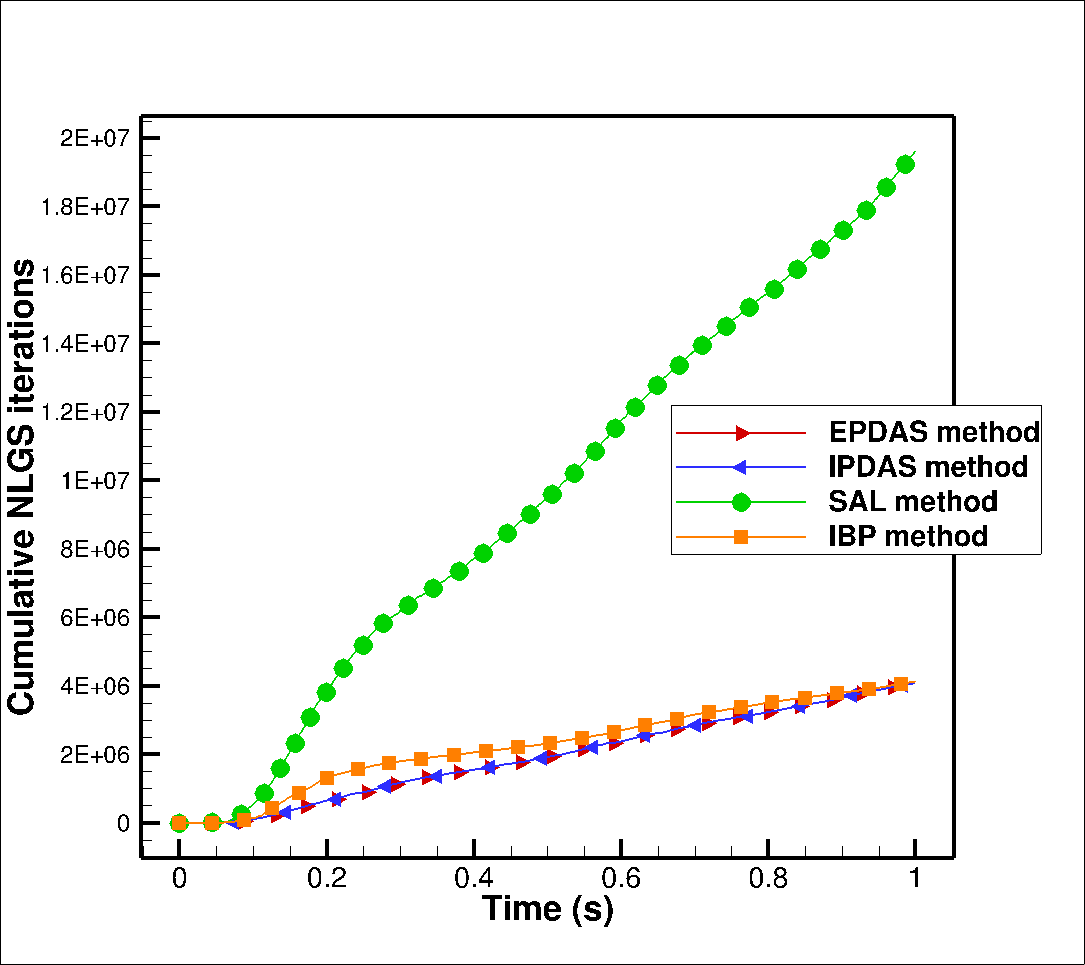
\includegraphics[width=0.32\textwidth]{chapitres/chapitre_3/figures/cumul_nlgs_tambour_400.png}}
\hspace{\fill}
   \subfloat[\label{cumul_cpu_nlgs_1600} ]{%
      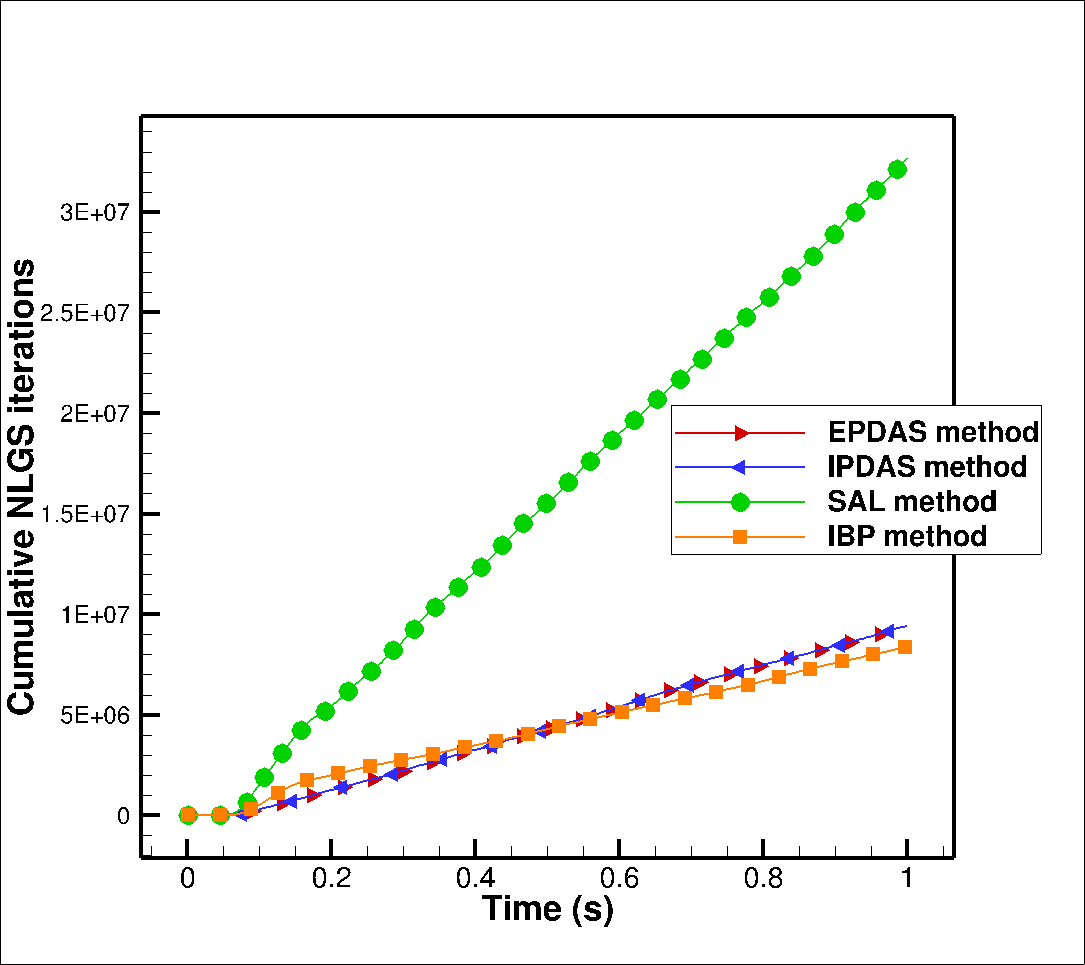
\includegraphics[width=0.32\textwidth]{chapitres/chapitre_3/figures/cumul_nlgs_tambour_1600.png}}\\
\caption{\label{cumul_nlgs_tambour}Evolution du nombre cumulé d'itérations NLGS nécessaire pour calculer les impulsions de contact lors de la simulation du tambour rotatif. (a) $100$ billes d'acier, (b) $400$ billes d'acier et (c) $1600$ billes d'aciers.}
\end{figure*}

\begin{table}[!h]
\begin{tabular}{|p{2cm}|p{1.75cm}|p{1.75cm}|p{1.75cm}|p{1.9cm}|p{1.9cm}|}
  \hline \rowcolor{lightgray}
  \multicolumn{6}{|c|}{Nombre total d'itérations NLGS} \\
  \hline \rowcolor{lightgray}
  Méthode numérique & 100 particules & 200 particules & 400 particules & 800 particules & 1600 particules \\ 
  \hline  EPDAS & $1680882$ & $2020349$ & $4069672$ & $5114280$ & $9422476$\\
  IPDAS & $1674177$ & $1933869$ & $4036740$ & $5036011$ & $9999666$\\
  SAL & $7836547$ & $8566285$ & $19607909$ & $15600032$ & $32656132$\\
  IBP & $1101849$ & $1340917$ & $4121136$ & $3688553$ & $8375264$\\ 
 \hline
\end{tabular}
 \caption{Nombre total d'itérations NLGS nécessaires au calcul des impulsions de contact lors de la simulation de tambour rotatif pour chaque méthode numérique et un nombre différent de billes d'acier.}\label{tab20}
\end{table}

En outre, les performances des méthodes PDAS pour de telles simulations sont assez remarquables par rapport aux méthodes SAL et IBP. Ci-dessous, nous fournissons les temps CPU totaux pour chaque simulation et chaque méthode numérique. Quel que soit le nombre de billes rigides impliquées dans le processus, les méthodes PDAS restent les moins coûteuses en temps de calcul. Comme nous pouvons le voir sur les graphes de la Figure \ref{cumul_cpu_tambour}, le temps CPU cumulé nécessaire pour calculer les impulsions de contact à l'aide des méthodes PDAS augmente légèrement avec le temps par rapport aux méthodes SAL et IBP. De plus, on peut remarquer d'après la Table \ref{tab21} que le temps CPU dépend fortement du nombre de billes rigides impliquées dans la simulation. En effet, plus nous avons de billes rigides dans le tambour rotatif, plus l'écart de temps CPU entre les méthodes numériques s'élargit, ce qui rend les méthodes PDAS plus pertinentes pour cet exemple.\\


\begin{figure*}[h!]
   \subfloat[\label{cumul_cpu_tambour_100}]{%
      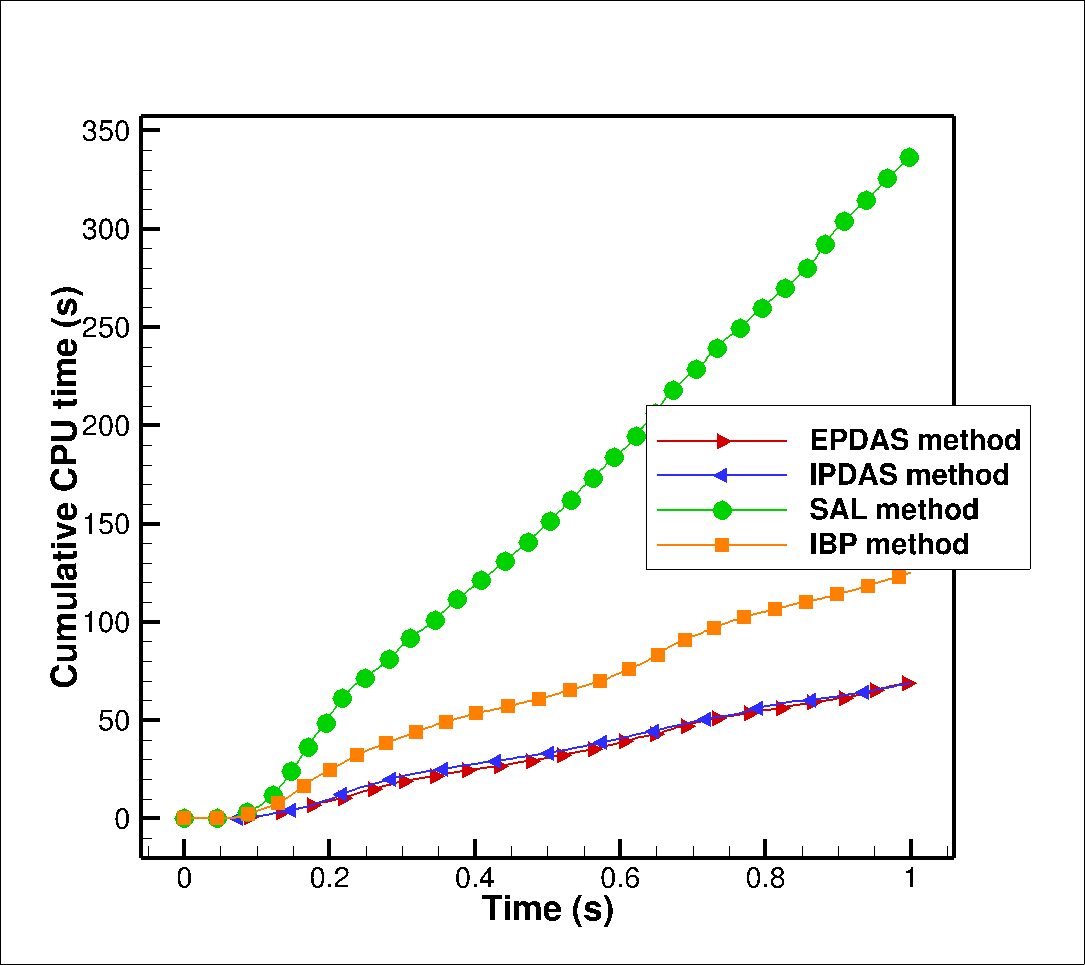
\includegraphics[width=0.32\textwidth]{chapitres/chapitre_3/figures/cumul_cpu_tambour_100.png}}
\hspace{\fill}
   \subfloat[\label{cumul_cpu_tambour_400} ]{%
      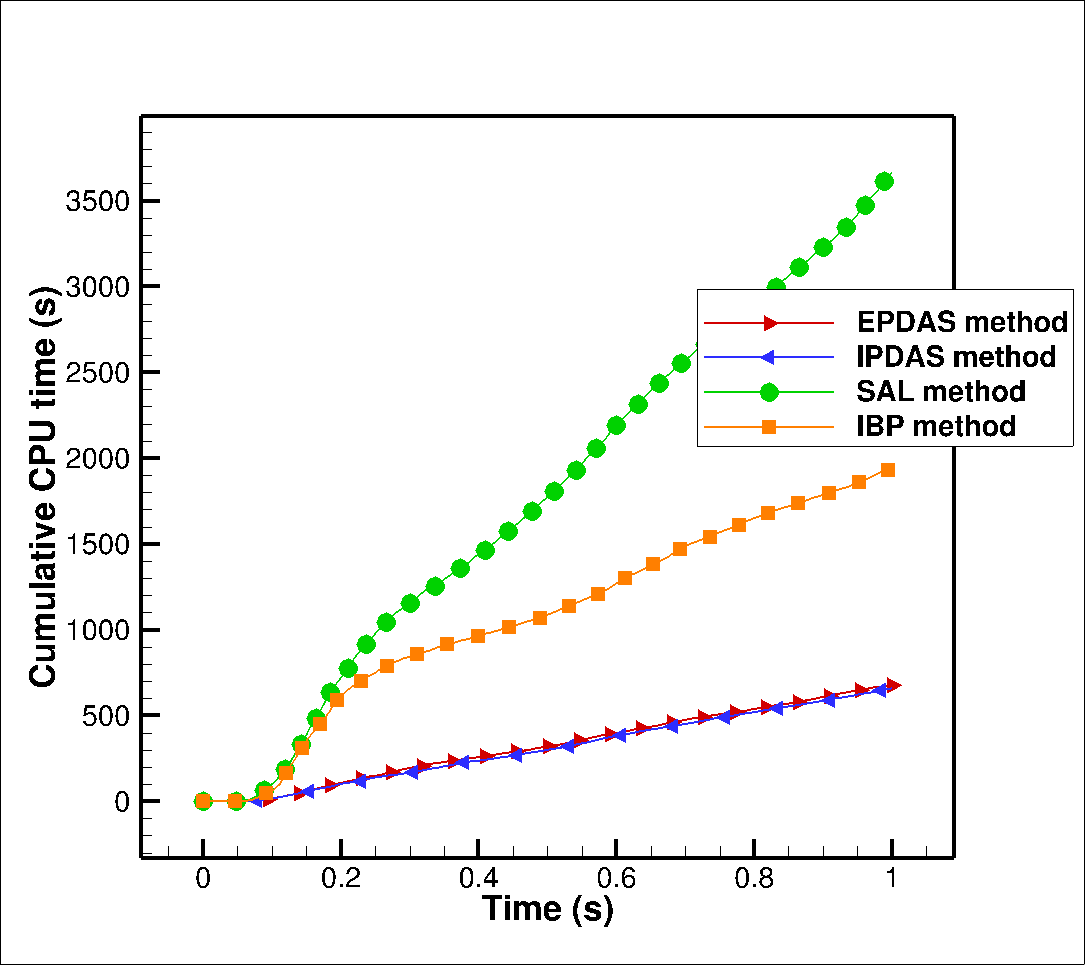
\includegraphics[width=0.32\textwidth]{chapitres/chapitre_3/figures/cumul_cpu_tambour_400.png}}
\hspace{\fill}
   \subfloat[\label{cumul_cpu_tambour_1600} ]{%
      \includegraphics[width=0.32\textwidth]{chapitres/chapitre_3/figures/cumul_cpu_tambour_1600.png}}\\
\caption{\label{cumul_cpu_tambour}Evolution du temps CPU cumulé nécessaire pour calculer les impulsions de contact lors de la simulation du tambour rotatif pour chaque méthode numérique. (a) $100$ billes d'acier, (b) $400$ billes d'acier et (c) $1600$ billes d'acier.}
\end{figure*}

\begin{table}[!h]
\begin{tabular}{|p{2cm}|p{1.75cm}|p{1.75cm}|p{1.75cm}|p{1.9cm}|p{1.9cm}|}
  \hline \rowcolor{lightgray}
  \multicolumn{6}{|c|}{Temps CPU total (s)} \\
  \hline \rowcolor{lightgray}
  Méthode numérique & 100 particules & 200 particules & 400 particules & 800 particules & 1600 particules \\ 
  \hline  EPDAS & $69.49$ & $163.92$ & $677.21$ & $1817.41$ & $7492.30$\\
  IPDAS & $68.81$ & $153.25$ & $657.01$ & $1804.86$ & $7867.88$\\
  SAL & $337.16$ & $755.55$ & $3663.25$ & $6055.49$ & $27425.82$\\
  IBP & $124.92$ & $259.37$ & $1941.16$ & $3232.92$ & $16740.52$\\ 
 \hline
\end{tabular}
 \caption{Temps CPU total consacré au calcul de la solution pour chaque méthode numérique.}\label{tab21}
\end{table}

\newpage

\section*{Conclusion}

Dans ce chapitre nous avons fournit dans un premier temps une extension du formalisme numérique PDAS pour le traitement des problèmes de contacts avec frottement en milieu granulaire. En effet, après avoir défini les conditions de contact avec frottement en mécanique non-régulière NSCD, un algorithme général a été détaillé pour traiter ces conditions numériquement. 
Une série de cas-test académiques couvrant un large éventail d'applications en milieu granulaire a été proposée dans un second temps pour évaluer la pertinence des méthodes PDAS.\\

\indent Premièrement, il s'avère que les méthodes Active Set sont plus efficaces en terme de convergence, puisqu'elles convergent plus rapidement comparées à la méthode du Lagrangien augmenté standard et du bi-potentiel amélioré. Deuxièmement, le gain en temps de calcul est très considérable, les méthodes Active Set étant plus rapides en termes de temps CPU. Troisièmement, les expériences numériques rapportées ci-dessus démontrent que les temps de calcul augmentent et ne sont plus comparables lorsque le nombre de corps rigides impliqués devient plus grand, mais restent toujours moins importants pour les méthodes PDAS.\\

\indent Ainsi, en vue des applications en milieu granulaire aux comportement complexes impliquant une multitude de corps rigides et un grand nombre de contacts simultanés, il serait pertinent d'envisager dans le chapitre suivant une comparaison applicative entre le formalisme numérique NSCD-PDAS et l'approche DEM-CUNDALL dans un environnement applicatif type industriel. Dans cette perspective, nous mettrons en oeuvre des cas-tests d'écoulements granulaires purs et de couplage fluide-milieu granulaire mettant en jeu énormément de corps rigides en interaction, ce qui nécessitera le recours aux paradigmes de parallélisation commun à toutes les applications industrielles et architectures exascales.